%%%%%%%%%%%%%%%%%%%%%%%%%%%%%%%%%%%%%%%%%%%%%%%%%%%%%%%%%%%%%%%%%%%%%
%%                                                                 %%
%% Please do not use \input{...} to include other tex files.       %%
%% Submit your LaTeX manuscript as one .tex document.              %%
%%                                                                 %%
%% All additional figures and files should be attached             %%
%% separately and not embedded in the \TeX\ document itself.       %%
%%                                                                 %%
%%%%%%%%%%%%%%%%%%%%%%%%%%%%%%%%%%%%%%%%%%%%%%%%%%%%%%%%%%%%%%%%%%%%%

%%\documentclass[referee,sn-basic]{sn-jnl}% referee option is meant for double line spacing

%%=======================================================%%
%% to print line numbers in the margin use lineno option %%
%%=======================================================%%

%%\documentclass[lineno,sn-basic]{sn-jnl}% Basic Springer Nature Reference Style/Chemistry Reference Style

%%======================================================%%
%% to compile with pdflatex/xelatex use pdflatex option %%
%%======================================================%%

%%\documentclass[pdflatex,sn-basic]{sn-jnl}% Basic Springer Nature Reference Style/Chemistry Reference Style

%%\documentclass[sn-basic]{sn-jnl}% Basic Springer Nature Reference Style/Chemistry Reference Style
\documentclass[pdflatex,sn-mathphys]{sn-jnl}% Math and Physical Sciences Reference Style

%%======================================================%%
%% Additional packages                                  %%
%%======================================================%%
\usepackage[nameinlink]{cleveref}
\usepackage{subcaption}
%%%% Standard Packages
%%<additional latex packages if required can be included here>
%%%%

\jyear{2023}%

%% as per the requirement new theorem styles can be included as shown below
\theoremstyle{thmstyleone}%
\newtheorem{theorem}{Theorem}%  meant for continuous numbers
%%\newtheorem{theorem}{Theorem}[section]% meant for sectionwise numbers
%% optional argument [theorem] produces theorem numbering sequence instead of independent numbers for Proposition
\newtheorem{proposition}[theorem]{Proposition}% 
%%\newtheorem{proposition}{Proposition}% to get separate numbers for theorem and proposition etc.

\theoremstyle{thmstyletwo}%
\newtheorem{example}{Example}%
\newtheorem{remark}{Remark}%

\theoremstyle{thmstylethree}%
\newtheorem{definition}{Definition}%

\raggedbottom
%%\unnumbered% uncomment this for unnumbered level heads

\begin{document}

\title[Spatially Adapted Statistical Segmentation]{Spatially Adapted Statistical Segmentation I:
  Reversing distortive X-ray effects for Accurate Implant-contact Tissue Classification in Bone SR$\mu$CT}

%%=============================================================%%
%% Prefix	-> \pfx{Dr}
%% GivenName	-> \fnm{Joergen W.}
%% Particle	-> \spfx{van der} -> surname prefix
%% FamilyName	-> \sur{Ploeg}
%% Suffix	-> \sfx{IV}
%% NatureName	-> \tanm{Poet Laureate} -> Title after name
%% Degrees	-> \dgr{MSc, PhD}
%% \author*[1,2]{\pfx{Dr} \fnm{Joergen W.} \spfx{van der} \sur{Ploeg} \sfx{IV} \tanm{Poet Laureate} 
%%                 \dgr{MSc, PhD}}\email{iauthor@gmail.com}
%%=============================================================%%


\author*[1,2,3]{\fnm{James} \sur{Avery}}\email{avery@ece.au.dk}
\author[1]{\fnm{Aleksandar} \sur{Topic}}\email{aleksandartpc@gmail.com}
\author[1,2]{\fnm{Carl-Johannes} \sur{Johnsen}}\email{carl-johannes@di.ku.dk}
\author[4]{\fnm{Else} \sur{Pinholt}}\email{empinholt@health.sdu.dk}
%\equalcont{These authors contributed equally to this work.}

\affil*[1]{\orgdiv{Niels Bohr Institute}, \orgname{University of Copenhagen}, \orgaddress{\street{Blegdamsvej 17}, \city{Copenhagen}, \postcode{2100}, \country{Denmark}}}

\affil[2]{\orgdiv{Dep. of Computer Science}, \orgname{University of Copenhagen}, \orgaddress{\street{Universitetsparken 5}, \city{Copenhagen}, \postcode{2100}, \country{Denmark}}}

\affil[3]{\orgdiv{Dep. of Electrical and Computer Engineering}, \orgname{Aarhus University}, \orgaddress{\street{Findlangsgade 22}, \city{Aarhus}, \postcode{8200}, \country{Denmark}}}

\affil[4]{\orgdiv{Dep. of Regional Health Research}, \orgname{University of Southern Denmark}}



%%==================================%%
%% sample for unstructured abstract %%
%%==================================%%

\abstract{
%TODO: Issue #2. Stram første paragraf.
Synchrotron Radiation micro-CT (SR$\mu$CT) produces 3D images at
extremely high fidelity.  However, while distortive X-ray effects such
as beam-hardening are minimized due to highly brilliant monochromatic
beams, they are not eliminated. In particular, obtaining accurate
tissue classification is a challenge near high-contrast interfaces
such as metal implants.

We present a computational method that discovers the image distortion as a function of space,
and produces continuous probabilistic models of material classification functions.
Using the derived models, we are able to accurately classify tissue throughout the full
image, even at high-contrast transition interfaces.
% 
We apply the method to solve the notoriously difficult problem of accurately classifying
biological tissue in contact with a titanium implant. 
  
%{\bf The data:}
The new tissue classification method was used to evaluate
bone-to-implant contact (BIC) in micrometer-resolution SR$\mu$CT images.
In a previous study, we were unable to obtain accurate
results for BIC, due to difficulties in accurately classifying the
tissue types near the titanium implant surface. In the present work,
we invert the distortive effects and obtain accurate tissue classification
all the way to the implant surface.
%TODO: Issue #1. MANGLER TAL HER. Disse skal beregnes.

The method is implemented in C++ and Python, and is parallelized for GPU and multi-core CPU.
To deal with the very large 3D image sizes arising from SR$\mu$CT, exceeding system
memory on even large workstations, the algorithms are designed to run
out-of-core on multi-resolution representations of the tomograms.
}

%%================================%%
%% Sample for structured abstract %%
%%================================%%

% \abstract{\textbf{Purpose:} The abstract serves both as a general introduction to the topic and as a brief, non-technical summary of the main results and their implications. The abstract must not include subheadings (unless expressly permitted in the journal's Instructions to Authors), equations or citations. As a guide the abstract should not exceed 200 words. Most journals do not set a hard limit however authors are advised to check the author instructions for the journal they are submitting to.
% 
% \textbf{Methods:} The abstract serves both as a general introduction to the topic and as a brief, non-technical summary of the main results and their implications. The abstract must not include subheadings (unless expressly permitted in the journal's Instructions to Authors), equations or citations. As a guide the abstract should not exceed 200 words. Most journals do not set a hard limit however authors are advised to check the author instructions for the journal they are submitting to.
% 
% \textbf{Results:} The abstract serves both as a general introduction to the topic and as a brief, non-technical summary of the main results and their implications. The abstract must not include subheadings (unless expressly permitted in the journal's Instructions to Authors), equations or citations. As a guide the abstract should not exceed 200 words. Most journals do not set a hard limit however authors are advised to check the author instructions for the journal they are submitting to.
% 
% \textbf{Conclusion:} The abstract serves both as a general introduction to the topic and as a brief, non-technical summary of the main results and their implications. The abstract must not include subheadings (unless expressly permitted in the journal's Instructions to Authors), equations or citations. As a guide the abstract should not exceed 200 words. Most journals do not set a hard limit however authors are advised to check the author instructions for the journal they are submitting to.}

\keywords{Image analysis, Tissue classification, Ossointegration, Segmentation, Bone-to-implant contact, Synchrotron Radiation micro-CT}

%%\pacs[JEL Classification]{D8, H51}

\pacs[MSC Classification]{92C55, 62H35}

\maketitle

\newcommand{\carl}[1]{}%\textcolor{orange}{[Carl: #1]}}
\newcommand{\aleksandar}[1]{}%\textcolor{cyan}{[Aleksandar: #1]}}
\newcommand{\james}[1]{}%\textcolor{red}{[James: #1]}}
\definecolor{ForestGreen}{RGB}{34,139,34}
\newcommand{\suggestion}[3]{}%\textcolor{ForestGreen}{[\textbf{Suggestion (#1):} '\sout{#2}' $\rightarrow$ '#3']}}


\newcommand{\xx}{\mathbf{x}}
% \newcommand{\fval}{f(\xx)}
% \newcommand{\fval}{f}
\newcommand{\fval}{x}
\newcommand{\lab}{\mathrm{L}}
\newcommand{\micron}{\ensuremath{\mu\text{m}}}
\newcommand{\Pof}[2]{P\!\left(#1\middle\vert #2\right)}
\newcommand{\voxels}{\mathsf{voxels}}
\newcommand{\field}{\mathsf{field}}

\section{Introduction}
\label{sec:intro}


\subsection{Image data}

Bone samples are most commonly analysed by extracting histologies and examining their
two-dimensional structure with light microscopy. This method has several drawbacks. First and
foremost, it is destructive: In addition to the obvious issue that the histology must be cut
from the full sample, the sawing process can contaminate soft tissue with bone dust, or leave
surface scratches that complicate automatic image analysis. Secondly, histology by its nature
only gives a two-dimensional slice of the full three-dimensional picture. Most important
biological structures are inherently three-dimensional, and limiting analysis to 2D severely
restricts the types of questions we can answer.

Synchrotron Radiation micro-tomography (SR$\mu$CT) offers a non-destructive high-quality
alternative to histology for detailed analysis of bone biopsies. \cite{torsten2018}
quantified the uncertainty of 2D histology for four common bone analyses, and found that the
choice of sampling plane for histological analysis incurred a significant uncertainty in the
results, whereas the full volumetric analysis of SR$\mu$CT tomograms did not.

The high brilliance and collimation of synchrotron radiation yields particularly
faithful 3D images, as common distortive X-ray effects seen in hospital-grade setups such
as beam hardening and projection artefacts are minimized. The high fidelity makes SR$\mu$CT
attractive for conducting advanced medical image analyses with trustworthy results.

However, while image distortion effects are much reduced compared to laboratory X-ray tomography,
they are not eliminated, and numerical analysis and computations on the images must still be
conducted carefully. Boundary effects near sample surfaces, ring artefacts from sensor faults, and especially
distortion near high-contrast transitions, make accurate tissue classification difficult in
regions where this distortion is significant. \cite{sporring} found that, while
they could accurately classify bone tissue in the middle regions of the tomograms, they were
not able to obtain good bone-to-implant contact evaluation (BIC), as evidenced by poor correlation
with histological analysis of the same samples.

The present work presents a fully automatic computational method which discovers probabilistic
models for the distortions incurred by the physical effects in high-resolution X-ray CT such
as SR$\mu$CT in order to reverse them and produce accurate tissue classification even in regions
where these effects are significant. It exploits two properties, which are needed to hold for
the method to work: i) very high resolution is used to build statistical models as functions
of space, and ii) the effects to be countered must vary continuously over space, so that we can
track how voxel frequency distributions are distorted throughout the image.
We apply the method to the
same dataset of micrometer-resolution SR$\mu$CT bone tomograms studied in \cite{torsten2018}
and in \cite{sporring}, to achieve faithful tissue classification all the way to the titanium
implant surface.

Our goal is to obtain good conditional probability distributions $\Pof{m\vert v}{\xx}$
that model the likelihood of a voxel having material type $m$ as a function
both on its value $v$ and its position $\xx$ in the tomogram. We want to make sure that these distribution
functions vary smoothly across space, to ensure that we can identify the materials correctly across the entire
image: even though the frequency distributions look completely different
close to the titanium implant compared to the middle region or sample surface,
we can track the unbroken, smooth deformation to assign a global material
identity.

The aims of the current work is:
\begin{enumerate}
\item To design a fully automatic \textbf{spatially aware segmentation algorithm} that
  improves segmentation quality of tissues in bone-SR$\mu$CT in all regions, including near high-contrast interfaces.
\item To implement this method efficiently in open-source software for GPU and multi-core CPU using out-of-core techniques, to
  facilitate analysis of 3D SR$\mu$CT images that exceed system memory.
\item To use the new method to evaluate bone-to-implant contact closer to implant surfaces than previously feasible. 
\end{enumerate}

\section{Background}
\label{sec:background}

%TODO: Rephrase
% In this section, we will briefly go through the physical composition of our samples, and how the
% data is acquired. Then we will look at the noise sources typical for this type of data, and show
% the effects that noise has on regions around the implant and biological tissue.

\subsection{Background for the medical experiment} Installation of a dental implant initiates the
Regional Acceleratory Phenomenon (RAP), which implies acceleration of the different healing stages.
RAP begins a few days after implant installation, peaks at 1-2 months, and subsides after 6-24
months~\cite{frost1989}. In cortical bone, the non-vital mineralized tissue initially needs to be
resorbed prior to bone formation. In the cancellous compartment, the implant installation mainly
results in damage of marrow spaces with resulting local bleeding and coagulum formation. The
coagulum gradually resorbs, collagen is laid down and replaced by osteoid, and eventually --- if
sufficient blood supply is present --- woven immature bone develops, and sequentially
osseointegration is initiated~\cite{frost1989}. After 6-12 weeks of healing most of the woven bone
is mineralized and bone marrow containing blood vessels, adipocytes, and mesenchymal cells can be
observed surrounding the trabeculae in the mineralized bone~\cite{Berglundh2003, Abrahamsson2004}.
A cement line, thickness  0.2-5µm, will be deposited directly on the implant surface during
continuous bone formation. The biological fixation of the implant initiates only a few days after
implant installation, where the osteoblasts begin to deposit collagen matrix on the cement line.
This early deposition of calcified matrix followed by the arrangement of woven bone and later mature
cancellous bone develops in a 3D manner delimiting the marrow space~\cite{Franchi2004}.

\subsection{Physical samples}

The experiment evaluated four methods for stimulating maxillary bone regeneration.  5 critical size
defects were introduced to 7 goats. Four defects were used to asses bone regeneration methods, and
one was a control sample.  Peri-implant vertical bone augmentation was performed using autologous
bone and two different calcium phosphate bone substitutes. The bone specimens were evaluated
undecalcified. The specimen preparation was performed at the Department of Biomaterials at
Gothenburg University, Sweden. The specimens were initially fixated in 4\% paraformaldehyde.
Dehydration of the specimens was performed in increasing concentrations of ethanol to eliminate fat
and water content. Furthermore, specimens were infiltrated with methylmethacrylate (MMA) and
embedded in molds 12 mm in diameter and 20 mm in height~\citep{NELDAM2015682}. They were scanned at
the European Synchrotron Radiation Facility (ESRF) in Grenoble, France.
The advantage of using MMA is greater tissue penetration than
water-soluble methacrylates.  This is an advantage when preparing larger specimens such as bone
biopsies containing dental implants. Furthermore, the histological quality of bone sections is
generally higher for MMA embedded specimens compared to water-soluble
methacrylates~\cite{erben1997}. Additionally, tissue shrinkage is less than 2\% when using MMA
embedded bone and cartilage specimens~\cite{ferguson1999}.

Physical samples were prepared for SR$\mu$CT scanning by cutting out portions from the larger
cylindrical biopsies. Within these samples, we find the titanium dental implant (Astra Tech
OsseoSpeed, ST Molndal, Sweden).  It is 3.5mm in diameter and 8mm long. Along its length the lower
5.5mm has larger threads and is attached to recipient bone. The upper 2.5mm has smaller threads and
is where newly formed bone is to be assessed. Surrounding the bone and implant contact-region are
cavities containing resin, air, blood vessels and other fibrous tissue.

\begin{figure}
  \centering
  \begin{tabular}{cc}
    (a) & \begin{tabular}{c} 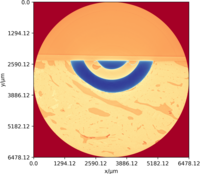
\includegraphics[width=0.5\textwidth]{770c_pag-full-xy-1x.png}\end{tabular}\\
    (b) & \begin{tabular}{c} 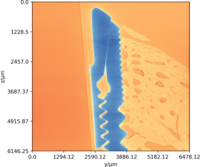
\includegraphics[width=0.5\textwidth]{770c_pag-full-yz-1x.png}\end{tabular}\\
    (c) & \begin{tabular}{c} 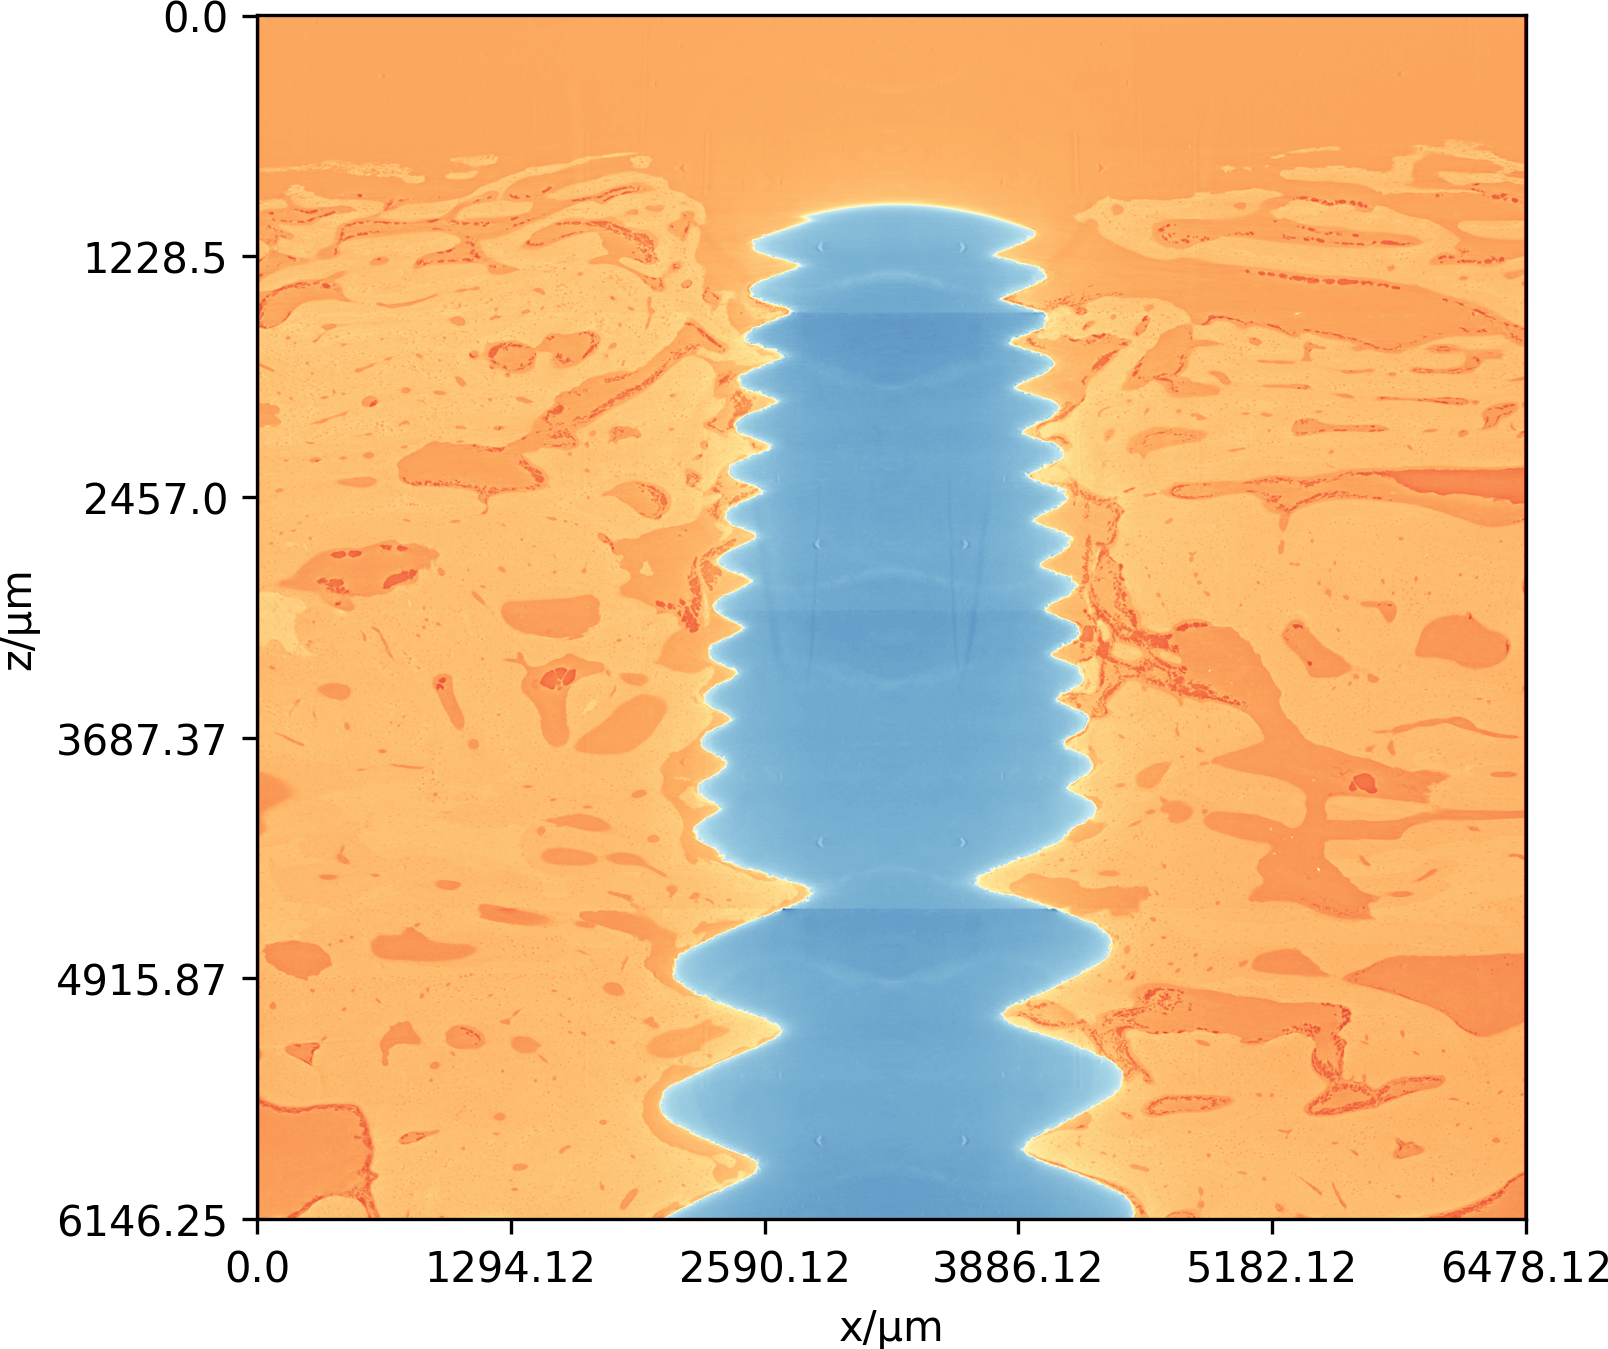
\includegraphics[width=0.5\textwidth]{770c_pag-full-xz-1x.png}\end{tabular}
  \end{tabular}
\caption{Cut sample seen as cross sections in XY, YZ and XZ-planes respectively. A voxel has a size
of 1.875$\mu$m. Red voxels are numerically low, while blue voxels are high.}
\label{fig:3viewsample}
\end{figure}

% TODO: description of color depends on final colormap -- still better than lighter/dark
A cut sample is shown in three different cross sectional views in \Cref{fig:3viewsample}. Each
material has a unique density and thus absorption. The titanium implant shown in blue has a higher
absorption level than bone. Bone material shown in light orange has higher absorption than its
surrounding dark orange colored regions containing blood vessels tissue, air and resin.

\subsubsection{Data acquisition}

It can be difficult to study and evaluate the bone structure and blood network without destroying or
manipulating the sample. X-ray computed tomography is a widely used tool for non-intrusive medical
imaging. By exposing a subject to X-rays, we can map the linear attenuation coefficient of the
passing rays. Each ray is attenuated relatively to the density and composition of the material it
passes.  By rotating either the scanner or the sample we can get a full 3D image representation of
the inner structure of the sample. Each volumetric pixel (voxel) then represents the X-ray
attenuation at its spatial position. In this way, X-rays can reliably be used to internally characterise
samples in a non-intrusive and non-destructive manner. Medical CT-scans can provide spatial
resolutions on the order of submillimetre scale \citep{medicalct}. The more modern micro computed
tomography ($\mu$CT) can provide much higher spatial resolution on the micrometre scale
\citep{srexptime}.

This work focuses on a data set acquired by Synchrotron Radiation micro-CT (SR$\mu$CT). For this
imaging technique, electrons are accelerated to ultra-relativistic speeds in trajectories directed
by strong magnetic fields. The resulting X-ray beam provides a high photon flux allowing for very
short exposure times \citep{srexptime}. This can help counter Poisson noise from suboptimal photon
count \citep{srnoise}. Contrary to both CT and $\mu$CT, this approach requires a large particle
accelerator, and is not standard medical or laboratory equipment. However, SR$\mu$CT  offers an even
better spatial resolution of up to 0.1 $\mu$m, and much higher image quality due to fewer distortive
X-ray effects. The resulting beams are high in brilliance and collimation, which gives a very clear
signal. Artifacts from beam-hardening are minimized due to synchrotron radiation X-rays being
characterized by their practically mono-energetic spectrum.

The tomograms presented here have been acquired at the ID19 beam line at the European Synchrotron
Radiation Facility (ESRF) in Grenoble, France. They were reconstructed\citep{sporring} at the ID19
beamline. A standard filtered back-projection algorithm was applied via the ESRF in-house developed
software PyHST~\citep{NELDAM2015682,pyhst}. PyHST was applied to improve reconstruction
quality, hence reducing ring artefacts, and to reduce the required data volume if
necessary~\cite{MIRONE201441}. The tomograms were acquired at 50 KeV.

\subsubsection{Image data}

The physical field-of-view of a single image sample is about 6.5mm in each direction. Each sample
contains voxels with a spatial resolution of 1.875$\mu$m. The samples are scanned in chunks of 4-6
sub-volumes through the height of the implant, depending on the initial size of a sample.

As the scans slightly overlap, we first compute the overlaps between
volumes, by shifting along the $Z$-axis until the square 3D image
differences are minimized over the overlap volume, producing the best
volume match. This allows us to combine the sub-volumes into a single coherent 3D image of the full sample.
The images are represented in a custom hierarchical image format to facilitate fast multiresolution analysis.
The full image has resolution $(3456,3456,3360)$ (ensured to be divisible by $32=2^5$), and
has 5 coarse layers at resolution divided by 2, 4, 8, 16, and 32.

%JA: Er ikke klar over, hvad der menes her! Kan redigeres og tilføjes igen senere.
% In image \Cref{fig:3viewsample} (YZ- and XZ-planes) we see dark edges around the border of
% the volume matched subvolumes at their overlaps. This creates an offset which is very prominent
% within the implant, but the large relative contrast due to its high density, makes this easier to
% ignore.  Even worse is the contribution of misrepresented voxels in the transitional regions where
% bone and tissue contains visible jagged edges.

\section{Physical effects}
\label{sec:physics}

Noise in tomography is unavoidable, and it makes segmentation harder because it further obscures the
boundaries between materials. Materials may be well separated from certain angles in the
3d-reconstructed image, but can overlap from others. Some noise like that corrected by flat-field
correction is very uniformly distributed across images. Other noise is however very spatially
dependent on its surrounding regions. Knowing the composition and positioning of the materials being
imaged, we can counter some of these effects during segmentation. The effects from noise manifest
themselves as numerical shifts in voxel-values as a function of their position. This is a direct
result of a misrepresented attenuation along the axis the X-rays are passing.

This dependency on orientation illustrates how voxel intensity values are not globally fixed.
Instead, how a certain material is represented in intensity, is highly dependent on its position
relative to neighbouring regions. Especially since this also determines the amount and type of
derived noise.  The same material with the same density, can thus be represented at multiple varying
intensities within the same sample.

% \begin{figure*} \centering 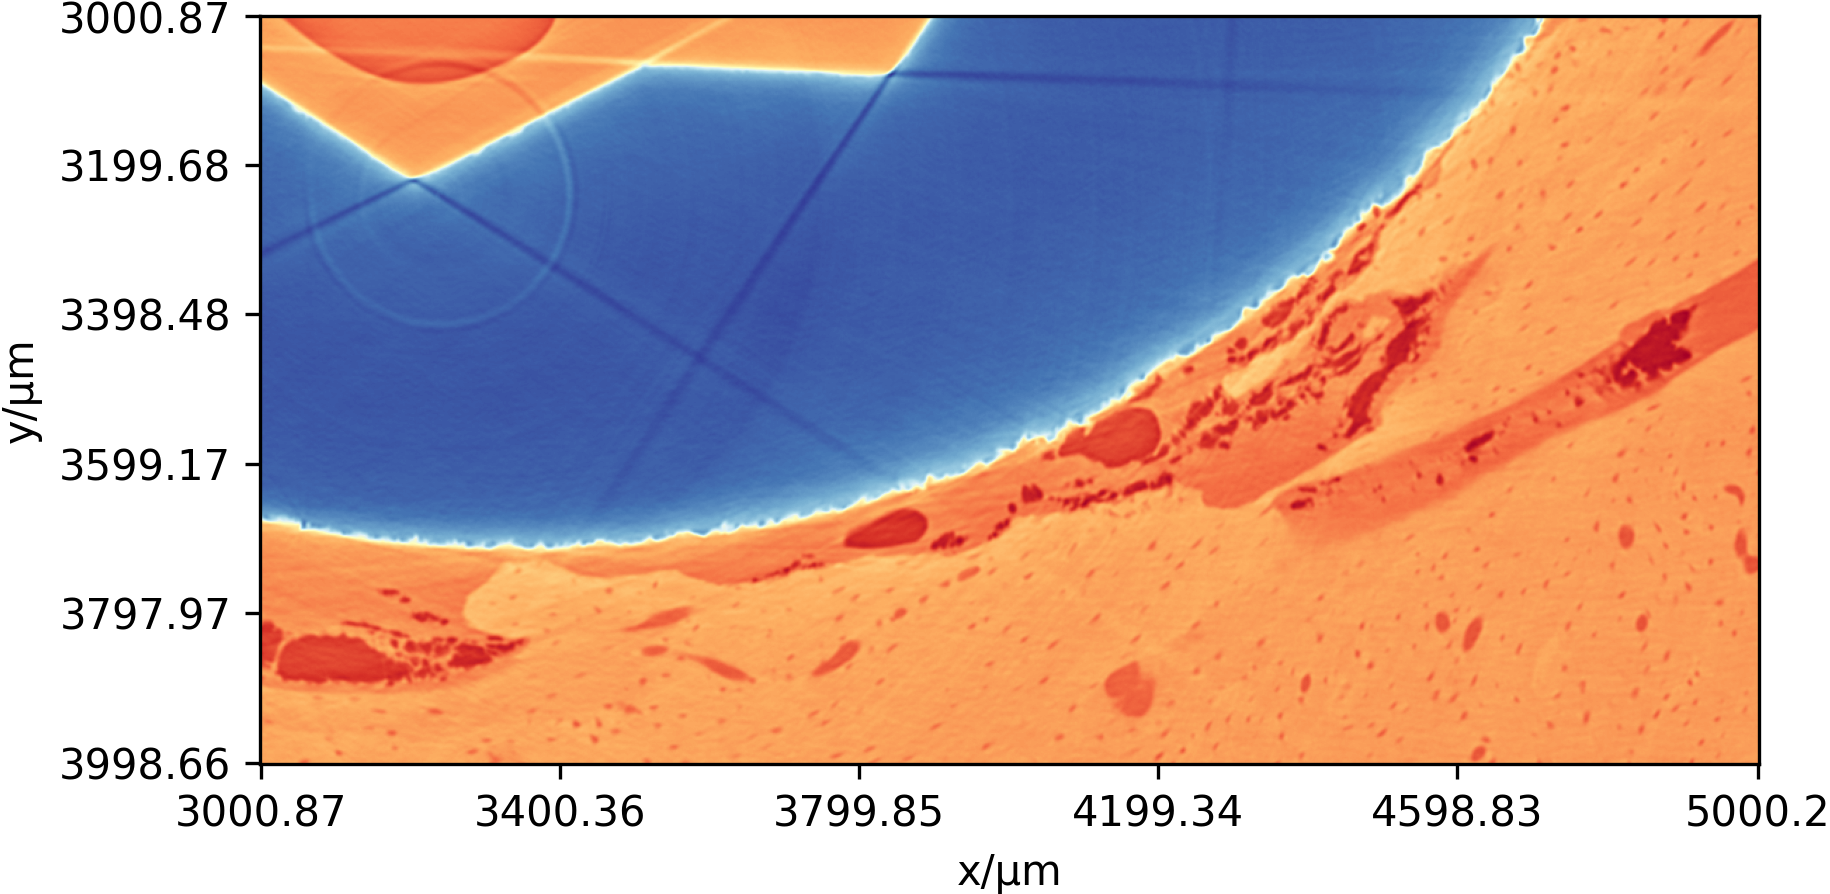
\includegraphics[width=\textwidth]{770c_pag-bic-xy-1x.png}
% \caption{Here we see a 1mm x 2mm region of an unscaled image slice in the XY dimension. It
% highlights some of the imperfections and noise present in the data. We especially see artifacts
% within and around the titanium implant.} \label{fig:xy-slice} \end{figure*}

\begin{figure}
  \centering
  \begin{tabular}{cc}
    \!\!\!\!\!\!(a)\!\!\!&\begin{tabular}{c}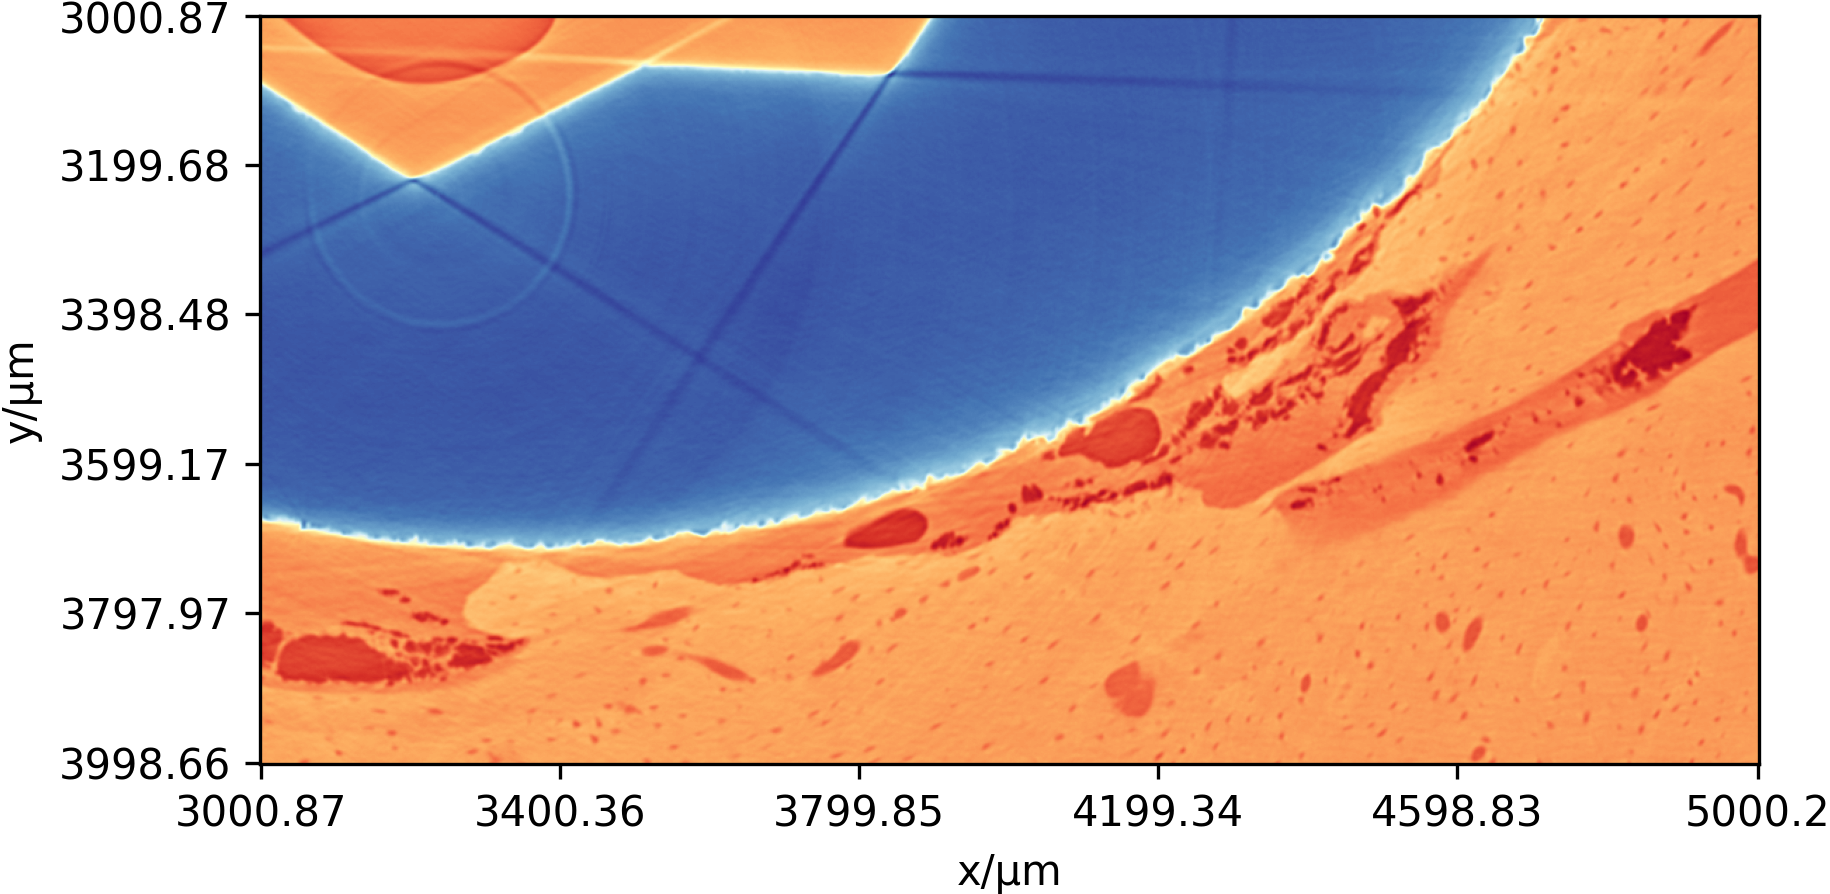
\includegraphics[width=0.96\columnwidth]{770c_pag-bic-xy-1x.png}\end{tabular}\\
    \!\!\!\!\!\!(b)\!\!\!&\begin{tabular}{c}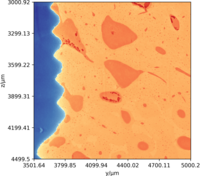
\includegraphics[width=0.96\columnwidth]{770c_pag-bic-yz-1x.png}\end{tabular}\\    
  \end{tabular}
  \caption{
    To better see the distortion effects, we zoom in on sub-regions of the slices shown in
    \Cref{fig:3viewsample}. Our visual systems automatically correct for most of the distortions,
    as they appear similar to illumination effects. However, even some distance from the implant,
    blood vessel voxels have higher values than bone voxels further out. As we approach the implant,
    the value-shifts accelerates and becomes highly non-linear.
    (a) A 1mm$\times$2mm region of an image slice in the XY-plane.
    % It highlights some of the imperfections and noise present in the data.
    (b) A 1.5mm x 1.5mm region of an image slice in the YZ-plane in the micro threaded part of
    the titanium implant.
  }
\label{fig:slices}
\end{figure}

In \Cref{fig:slices}, we see zoomed in regions of the XY- and YZ-planes of the same sample as shown
in \Cref{fig:3viewsample}.  Both planes display a broad selection of the various type of noise
sources found in the data.

\paragraph{Beam hardening}
Medical CT and $\mu$CT both utilize poly-energetic beams, which can cause artefacts around high
density regions. This effect is called beam-hardening \citep{beam-hardening}, and occurs when rays
with lower energy are attenuated more frequently, thus shifting the remaining photon energy to a
higher effective average value. This offsets the local contrast, by overestimating the attenuation,
leaving lighter spots on the image. Many types of artefacts will typically be present in X-ray 
setups, but most are taken into account by calibration using phantoms and pre-hardening the beam
before it reaches the sample. Pre-hardening of the beam is done using filters that attenuate the
softest rays. Due to its common usage, various metal artefact reduction (MAR) software exists to
account for noise and imperfections during reconstruction \citep{mar1}\citep{mar2}.

Despite the practically mono-energetic rays from SR$\mu$CT, the source initially generates a
poly-chromatic spectrum. During monochromatisation the resulting spectrum can still contain
corrupted harmonic components. Only a few percent corruption is enough to produce strong artefacts,
although monochromatisation is typically done in multiple layers \citep{srnoise}.  It can not
trivially be rejected that some noise does occur from poly-energetic incident radiation.  Two
distinct effects typically seen as a result of beam-hardening are in dark and bright streaks and
cupping artefacts in high density regions.

\paragraph{Dark and bright streaks} Streaking artefacts occur at the dense implant region, but also
in the transition from bone to softer tissue. This effect is mostly seen in regions of large
heterogeneity. When X-ray beams pass at angles containing multiple dense obstacles, the beam is
hardened more. Then for angles with fewer dense obstacles the energy spectrum is preserved better.
This produced the dark and bright streaks seen in \Cref{fig:slices}.

For a hardened beam, softer x-rays are absorbed instead of successfully penetrating the object, and
will not contribute to image formation. High density structures such as the titanium implant break
the isotropy, making the projected X-ray mean energy spectrum dependent on incident orientation
\citep{srnoise}.

\paragraph{Cupping effect} A common artefact that occurs when beams pass more homogeneous
cylindrical objects. Since beams passing the middle will traverse more material compared to the
edges, the beam is hardened more towards the center and intensity becomes lower as a result. This
can manifest itself in what erroneously looks to be dense peripheral regions at the edges.

\paragraph{Phase contrast} Phase contrast is an effect whose consequences are not very unlike those
of beam-hardening.  Although used as an advantage in holotomography\citep{holotomography} and phase
contrast tomography\citep{phasecontrast}, it induces noise in regular tomography such as used here.
It typically results in fringes around edges of regions within the image\citep{srnoise}. Similar to
dark and bright streaks mentioned above, they show as misrepresentations of the voxel values. In our
case we see them especially at the transitional edges between the titanium implant and the
biological tissue and bone.

\subsection{Other noise and artifacts}
\label{sec:noise-artefacts}

\paragraph{Ring artefacts} Looking at the XY-plane in \Cref{fig:slices}(a) we see clear concentric ring
artefacts emanating from the center of the sample, and at strong edges of the titanium implant. It
propagates strongly through the large region of air behind the implant. Compared to the other
artefacts mentioned, this effect is arising from imperfections in the scanner setup. These types of
artefacts can typically come from uncalibrated or defect adjacent detector elements. For synchrotron
radiation sources it can also occur from shifts and vibrations in the monochromator crystal
\citep{ringartefacts}.

\paragraph{Projection artefacts} Bright streaks with strong edges are seen from the sharp corners of
the titanium implant. When doing back projection, a symmetry break is seen as smeared lines across
the sample. This can occur from the high pass filter used during filtered back projection, which
exaggerates the differences between adjacent elements \citep{ctnoise}.

\paragraph{Compton scattering} Lower energy rays contribute mostly with noise from scattering
effects. A ray will propagate through a material, get scattered and diffract from its initial
trajectory. This gives a misrepresentation of the attenuation along its initial trajectory. The
artefacts seen from scattering are similar in nature to those formed by beam hardening. This is
because both phenomena effectively reduce the measured attenuation. For energy levels relevant for
the data presented here, of 50 KeV and above, Compton scattering is the dominant type
\citep{Compton}.  The scattering occurs due to photon-electron interaction between X-ray beam and
the material it passes through. Like beam-hardening, scattering will cause dark streaks across the
image, where attenuation was highest.

\subsection{Dealing with artefacts}
\label{sec:dealwithit}

The distortions that come from the class of physical effects and noise artefacts discussed in this
section, will vary continuously as a function of the spatial coordinates. This allows the possibility
for a method, which can correctly identify materials despite varying voxel values.
% FIXME: Would like a reference for the continous argument
% It is also mentioned in the last sentences of the first paragraph in
% "Physical effects, noise and artifacts"

%Partial volume artefacts which are dependent on the voxel size and are mentioned briefly by Neldam et al.

\section{Method}\label{sec:method}
% Spatial correlation 2d histograms (den nemme, 1 2d hist)
In this section, we will describe the method for exploiting spatial correlation based on the
2D-histograms of the tomographies. We will start by motivating the problem, then give an overview
of how we solve the problem, with a final detailed walk-through of each step in the overall workflow.

\subsection{1-dimensional histograms}
%diskuter overlappende materialer
Looking at a 1D-histogram of the voxel value in a tomography, as shown in~\Cref{fig:1d-hist}, we are
able to distinguish different distributions, but we see that there are large overlaps. This leads to
global thresholding being infeasible, at least for the distributions in the lower half of the histogram.
This happens because the voxel value is not globally defined, as~\Cref{sec:physics} explains, which
illustrates how the different materials cover ranges of values that blend together in the histogram.

\begin{figure}
    \centering
    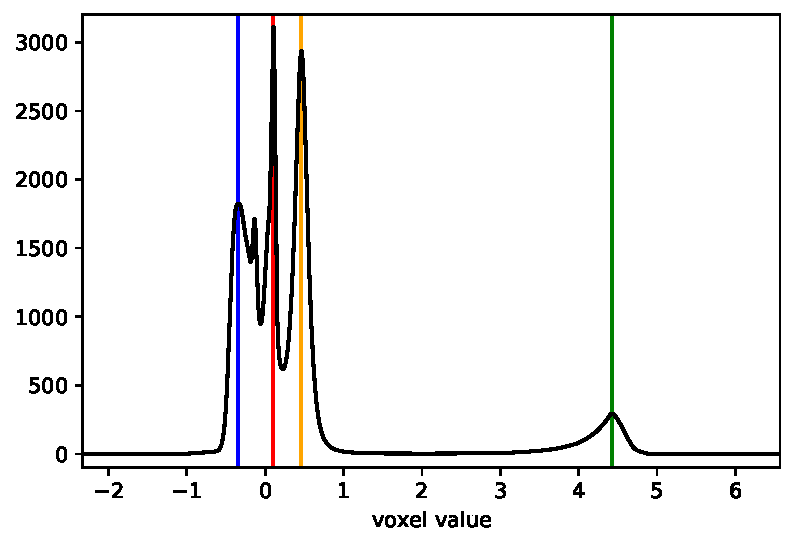
\includegraphics[width=\linewidth]{1d_hist.pdf}
    \caption{1-dimensional histogram of the voxel values of a tomography. The blue line is air peak,
    the red line is the soft tissue peak, the green line is the bone peak, and the orange line is
    the implant peak.}
    \label{fig:1d-hist}
\end{figure}

\subsection{Preprocessing}\label{sec:preprocess}
To reduce the complexity of the segmentation process, we preprocess
the data by removing redundant information.
% Since the values of the implant material is well-separated from the rest of the sample, obtaining
% the rough implant mask through global thresholding is trivial, as the orange line in~\Cref{fig:1d-hist}
% shows. This mask is then refined, along with the internal gaps being closed, giving us the implant mask.
We first compute a coarse
bone-region using a crude segmentation, and through a direct geometric
analysis of the implant determines the sample coordinate system, with the origin
on the back-plane of the sawed-through implants and principal axes coordinate system vectors
$\mathbf{u}$ pointing up towards the implant top, $\mathbf{v}$ pointing forward away from the back-plane,
and $\mathbf{w}$ point right, parallel to the back-plane. An automatic wave-analysis of the threads
computationally determines the macro-threaded recipient bone region, and the micro-threaded de-novo regenerated bone region.
We then perform the spatially-aware segmentation analysis restricted to the bone-regions in order to
not expand effort on the parts of the segmentation problem that can be solved with simpler methods.
Note that the process is fully automatic, and does not require human intervention.

%TODO: Måske medtage disse detaljer, men er for træt til at renskrive.
% , we are also able to remove the air making up half of the sample cylinder. This is depicted
% in~\Cref{fig:3viewsample}, above the implant and to the left of the implant in the XY and YZ cross
% sections respectively. Finally the implant mask can show us the orientation of the implant. This squashes
% the blue peak from the histogram, leaving the two peaks marked by the red and green lines as being
% the most defined.

% As we are only interested in the voxels inside the bone, and we know that bone is the most prominent
% material left, we perform another coarse segmentation. This is done by thresholding between the two
% large distributions, choosing everything to the right of this threshold as the bone mask. These voxels
% are morphologically closed, to also consumes the internal gaps in the bone region, which makes up the
% soft tissue inside the bone. The implant and bone region masks are applied throughout subsequent steps
% to filter out noise in the tomography.

\subsection{Exploiting spatial information}
% Show the correlation of x,y,z,r to histograms 2d
Our goal is to discover how the value distributions for the different materials -- bone, blood vessels, etc. --
change as a function of space. In other words, we wish to uncover information about the conditional probabilities $\Pof{m}{v,\xx}$ that a voxel with value $v$ and
position $\xx$ represents material $m$. We cannot compute this directly using only the image, as only one voxel occupies position $\xx$. 

However, if we fix one axis $x$, $y$, or $z$, the image {\em does} contain millions of voxels with that fixed value, enough to make good statistical
models for e.g.~the conditional probabilities $\Pof{m}{v,x}$, $\Pof{m}{v,y}$, and $\Pof{m}{v,z}$. To this end, we compute 2D histograms that simply count voxel frequencies
both conditioned on value $v$ and coordinate value along either $x$, $y$, or $z$. 

Figure \ref{fig:2dhists}(a)
shows the histogram for our model tomogram (implant excluded) as a function of the $y$ coordinate: each row in the image is a histogram for a fixed value of $y$.
Figure \ref{fig:3viewsample}(a) helps us see what happens: For $y<2400\micron$, there is only air, then we reach a thin layer of resin, after which we enter
the region where we find bone, soft tissue, resin, and air. The air voxels are brightened as we approach the implant, shifting the peaks smoothly rightwards.
Figure \ref{fig:2dhists}(b) shows a similar 2D histogram for the radial coordinate $r=\sqrt{x^2+y^2+z^2}$.
From this plot, we see two prominent distributions that change along the $r$ axis. The radius correlates with distance to the sample surface
(capturing edge effects), and for medium $r$, it is a good proxy for distance to the implant, and we see a brightening with smaller $r$, and a darkening and
broadening of the distributions for large $r$. Each {\em view} provides us with additional information about how voxel values are distorted throughout space:
analogous to casting shadows along different axes to obtain more information about a 3D object. We can either use Bayesian statistics to combine information
from multiple axes, or construct a spatial grouping that is particularly suited to capture the effects of the distortive effects that we want to counter.
The next section describes the latter.

% Kept for historical reasons.
%\begin{algorithm}
%    \caption{2-dimensional histograms. Allocation also implies zero initialization.}
%    \label{alg:2dhists}
%    \begin{algorithmic}
%        \Function {2D\_hist} {$\voxels[n_z,n_y,n_x],c_x,c_y,n_{bins},v_{min},v_{max}$}
%            \State $n_r \gets \left\lfloor\sqrt{\left\lfloor \frac{n_x}{2} \right\rfloor^2 + \left\lfloor \frac{n_y}{2} \right\rfloor^2}\right\rfloor+1$
%            \State \textbf{allocate} $h_z[n_z,n_{bins}], h_y[n_y,n_{bins}]$
%            \State \textbf{allocate} $h_x[n_x,n_{bins}], h_r[n_r,n_{bins}]$
%            \For {$z,y,x$ \textbf{in} $0{:}n_z,0{:}n_y,0{:}n_x$}
%                \State $v \gets \voxels[z,y,x]$
%                \If {$v_{min} \leq v \leq v_{max}$}
%                    \State $v_{i} \gets (n_{bins}-1) \cdot \frac{v - v_{min}}{v_{max} - v_{min}}$
%                    \State $r \gets \left\lfloor\sqrt{(x-c_x)^2 + (y-c_y)^2}\right\rfloor$
%                    \State $h_z[z,v_{i}]{+}{+}$
%                    \State $h_y[y,v_{i}]{+}{+}$
%                    \State $h_x[x,v_{i}]{+}{+}$
%                    \State $h_r[r,v_{i}]{+}{+}$
%                \EndIf
%            \EndFor
%            \Return $h_z,h_y,h_z,h_r$
%        \EndFunction
%    \end{algorithmic}
%\end{algorithm}

\begin{algorithm}
    \caption{2-dimensional radius histogram.}
    \label{alg:2dhists}
    \begin{algorithmic}
        \Function {hist\_r} {$|voxels|[n_z,n_y,n_x],c_x,c_y,n_{bins},v_{min},v_{max}$}
            \For {$z,y,x$ \textbf{in} $0{:}n_z,0{:}n_y,0{:}n_x$}
                \State $v \gets |voxels|[z,y,x]$
                \If {$v_{min} \leq v \leq v_{max}$}
                    \State $v_{i} \gets (n_{bins}-1) \cdot \frac{v - v_{min}}{v_{max} - v_{min}}$
                    \State $r \gets \left\lfloor\sqrt{(x-c_x)^2 + (y-c_y)^2}\right\rfloor$
                    \State $h_r[r,v_{i}]{+}{+}$
                \EndIf
            \EndFor\\
            \Return $h_r$
        \EndFunction
    \end{algorithmic}
\end{algorithm}

\begin{figure}
    \centering
    %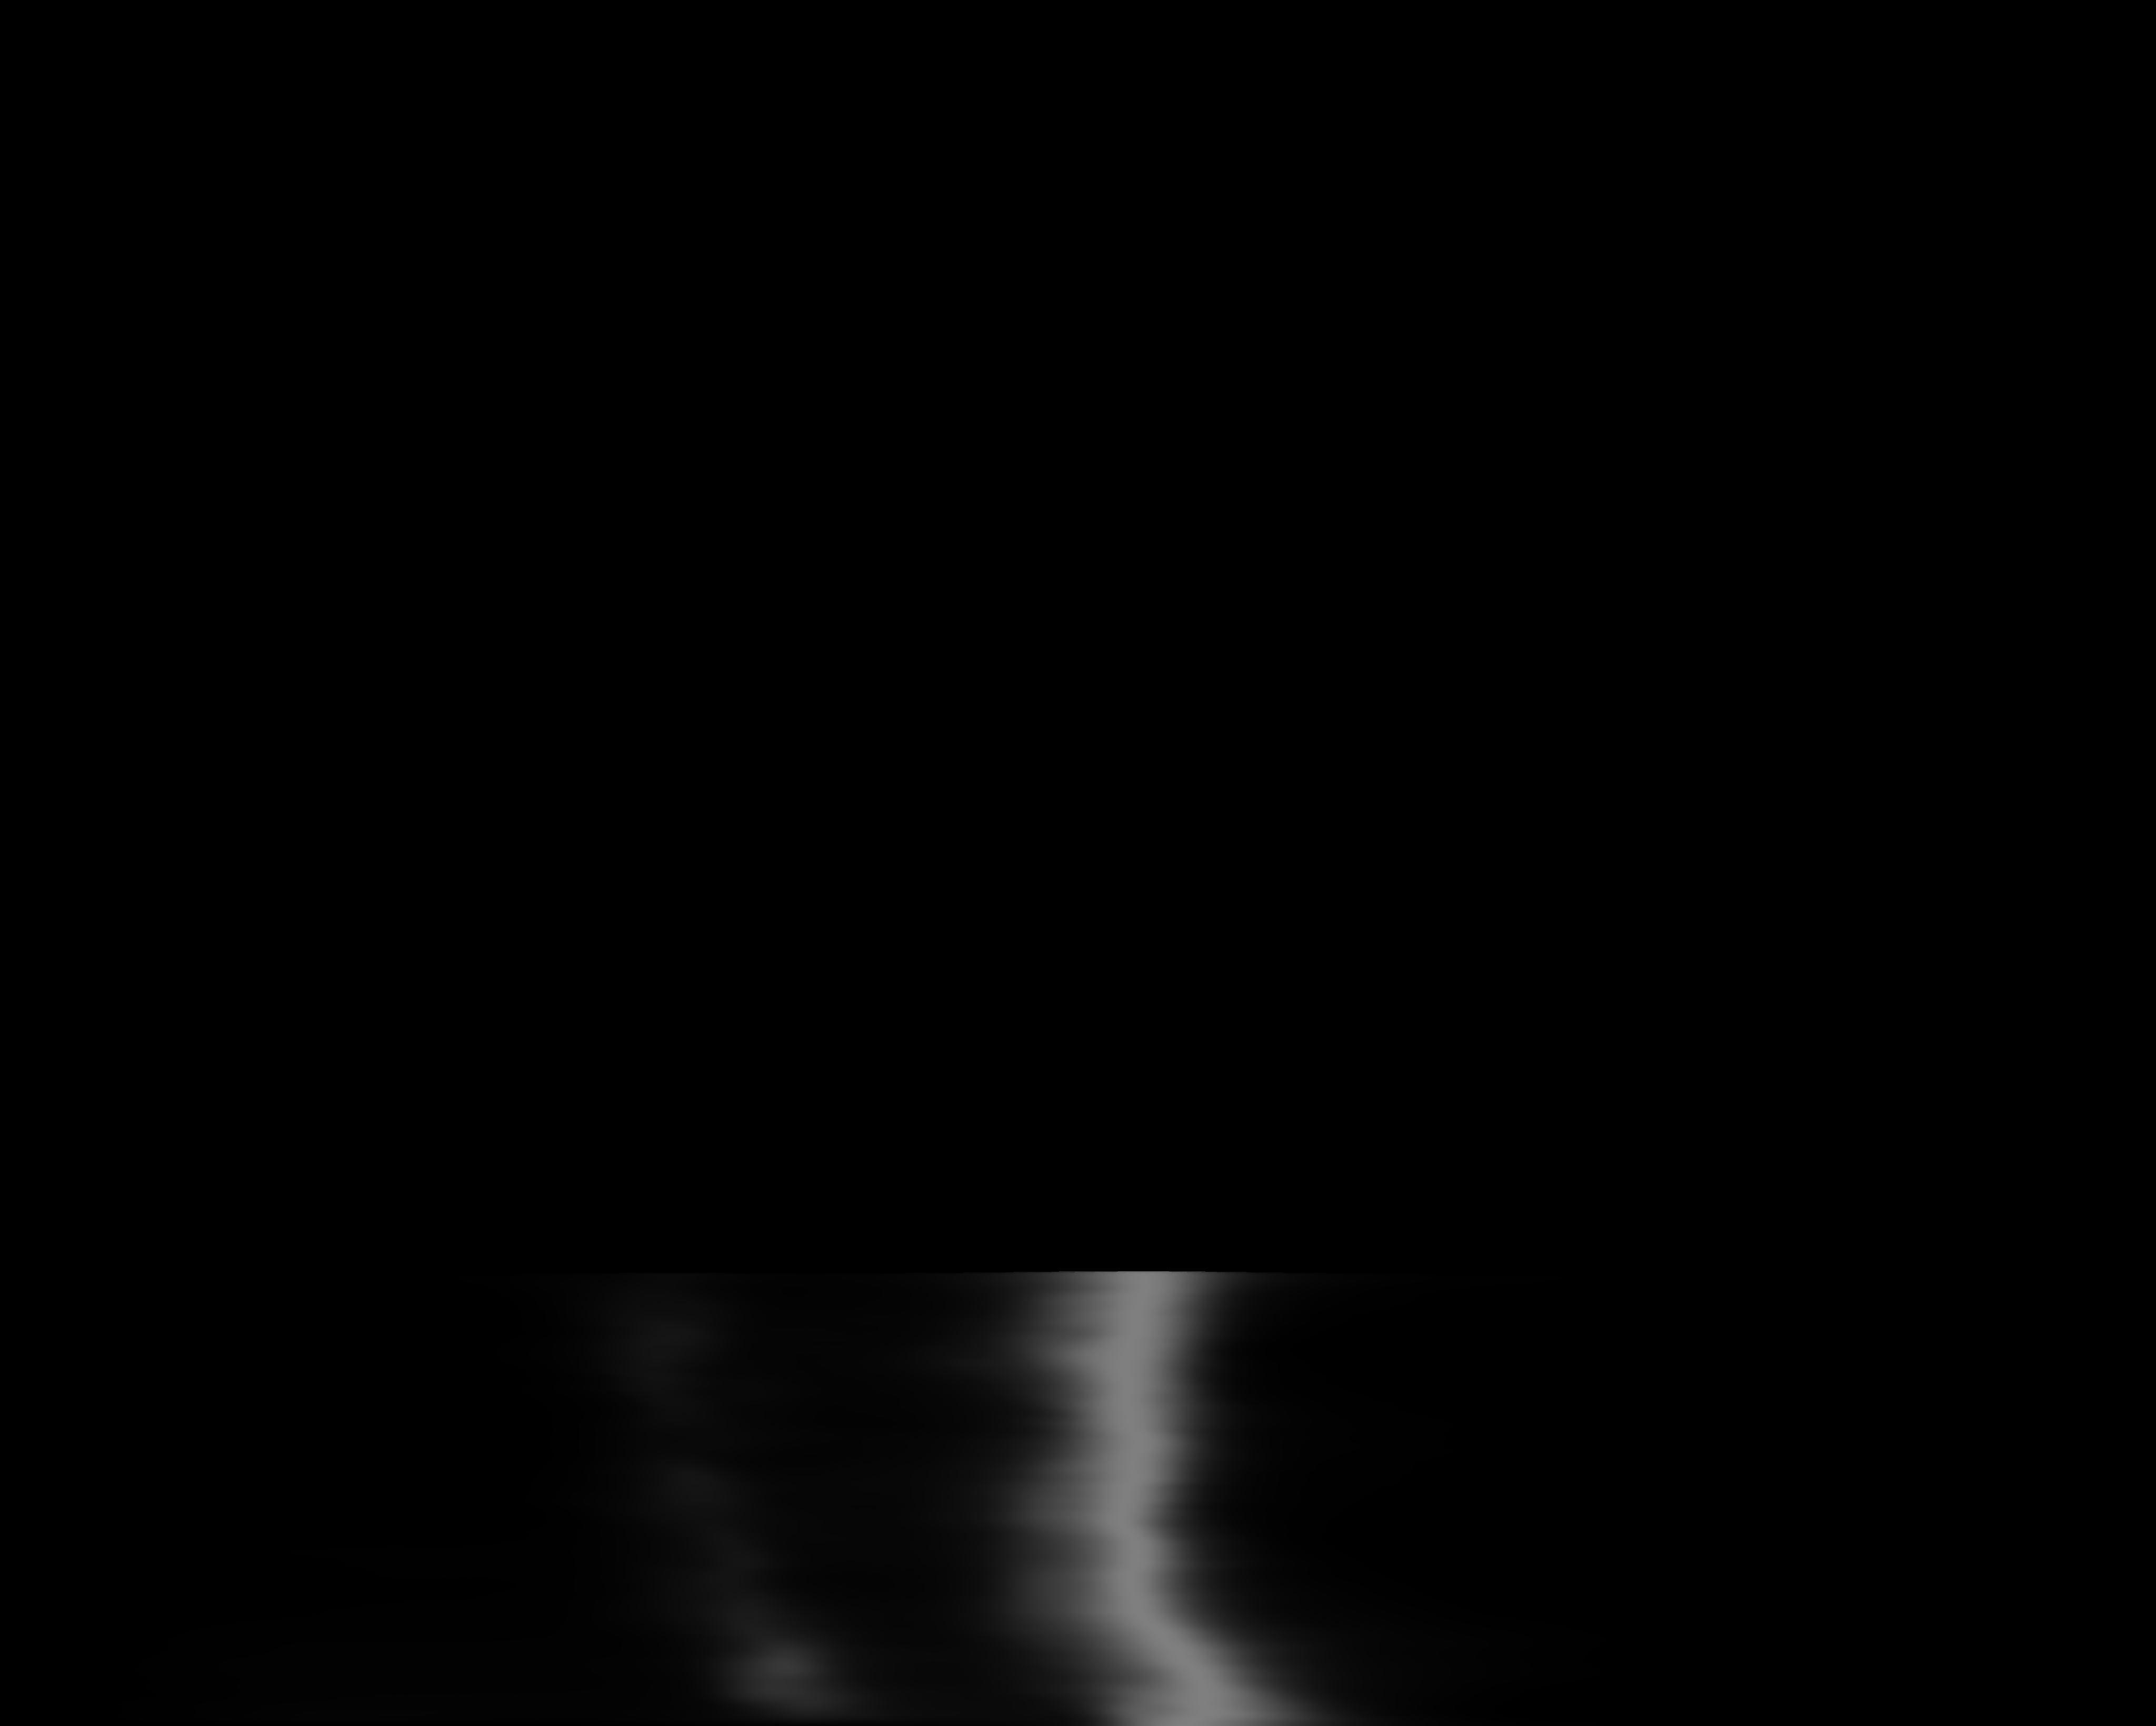
\includegraphics[width=.49\linewidth]{zb-bone_region3.png}
    %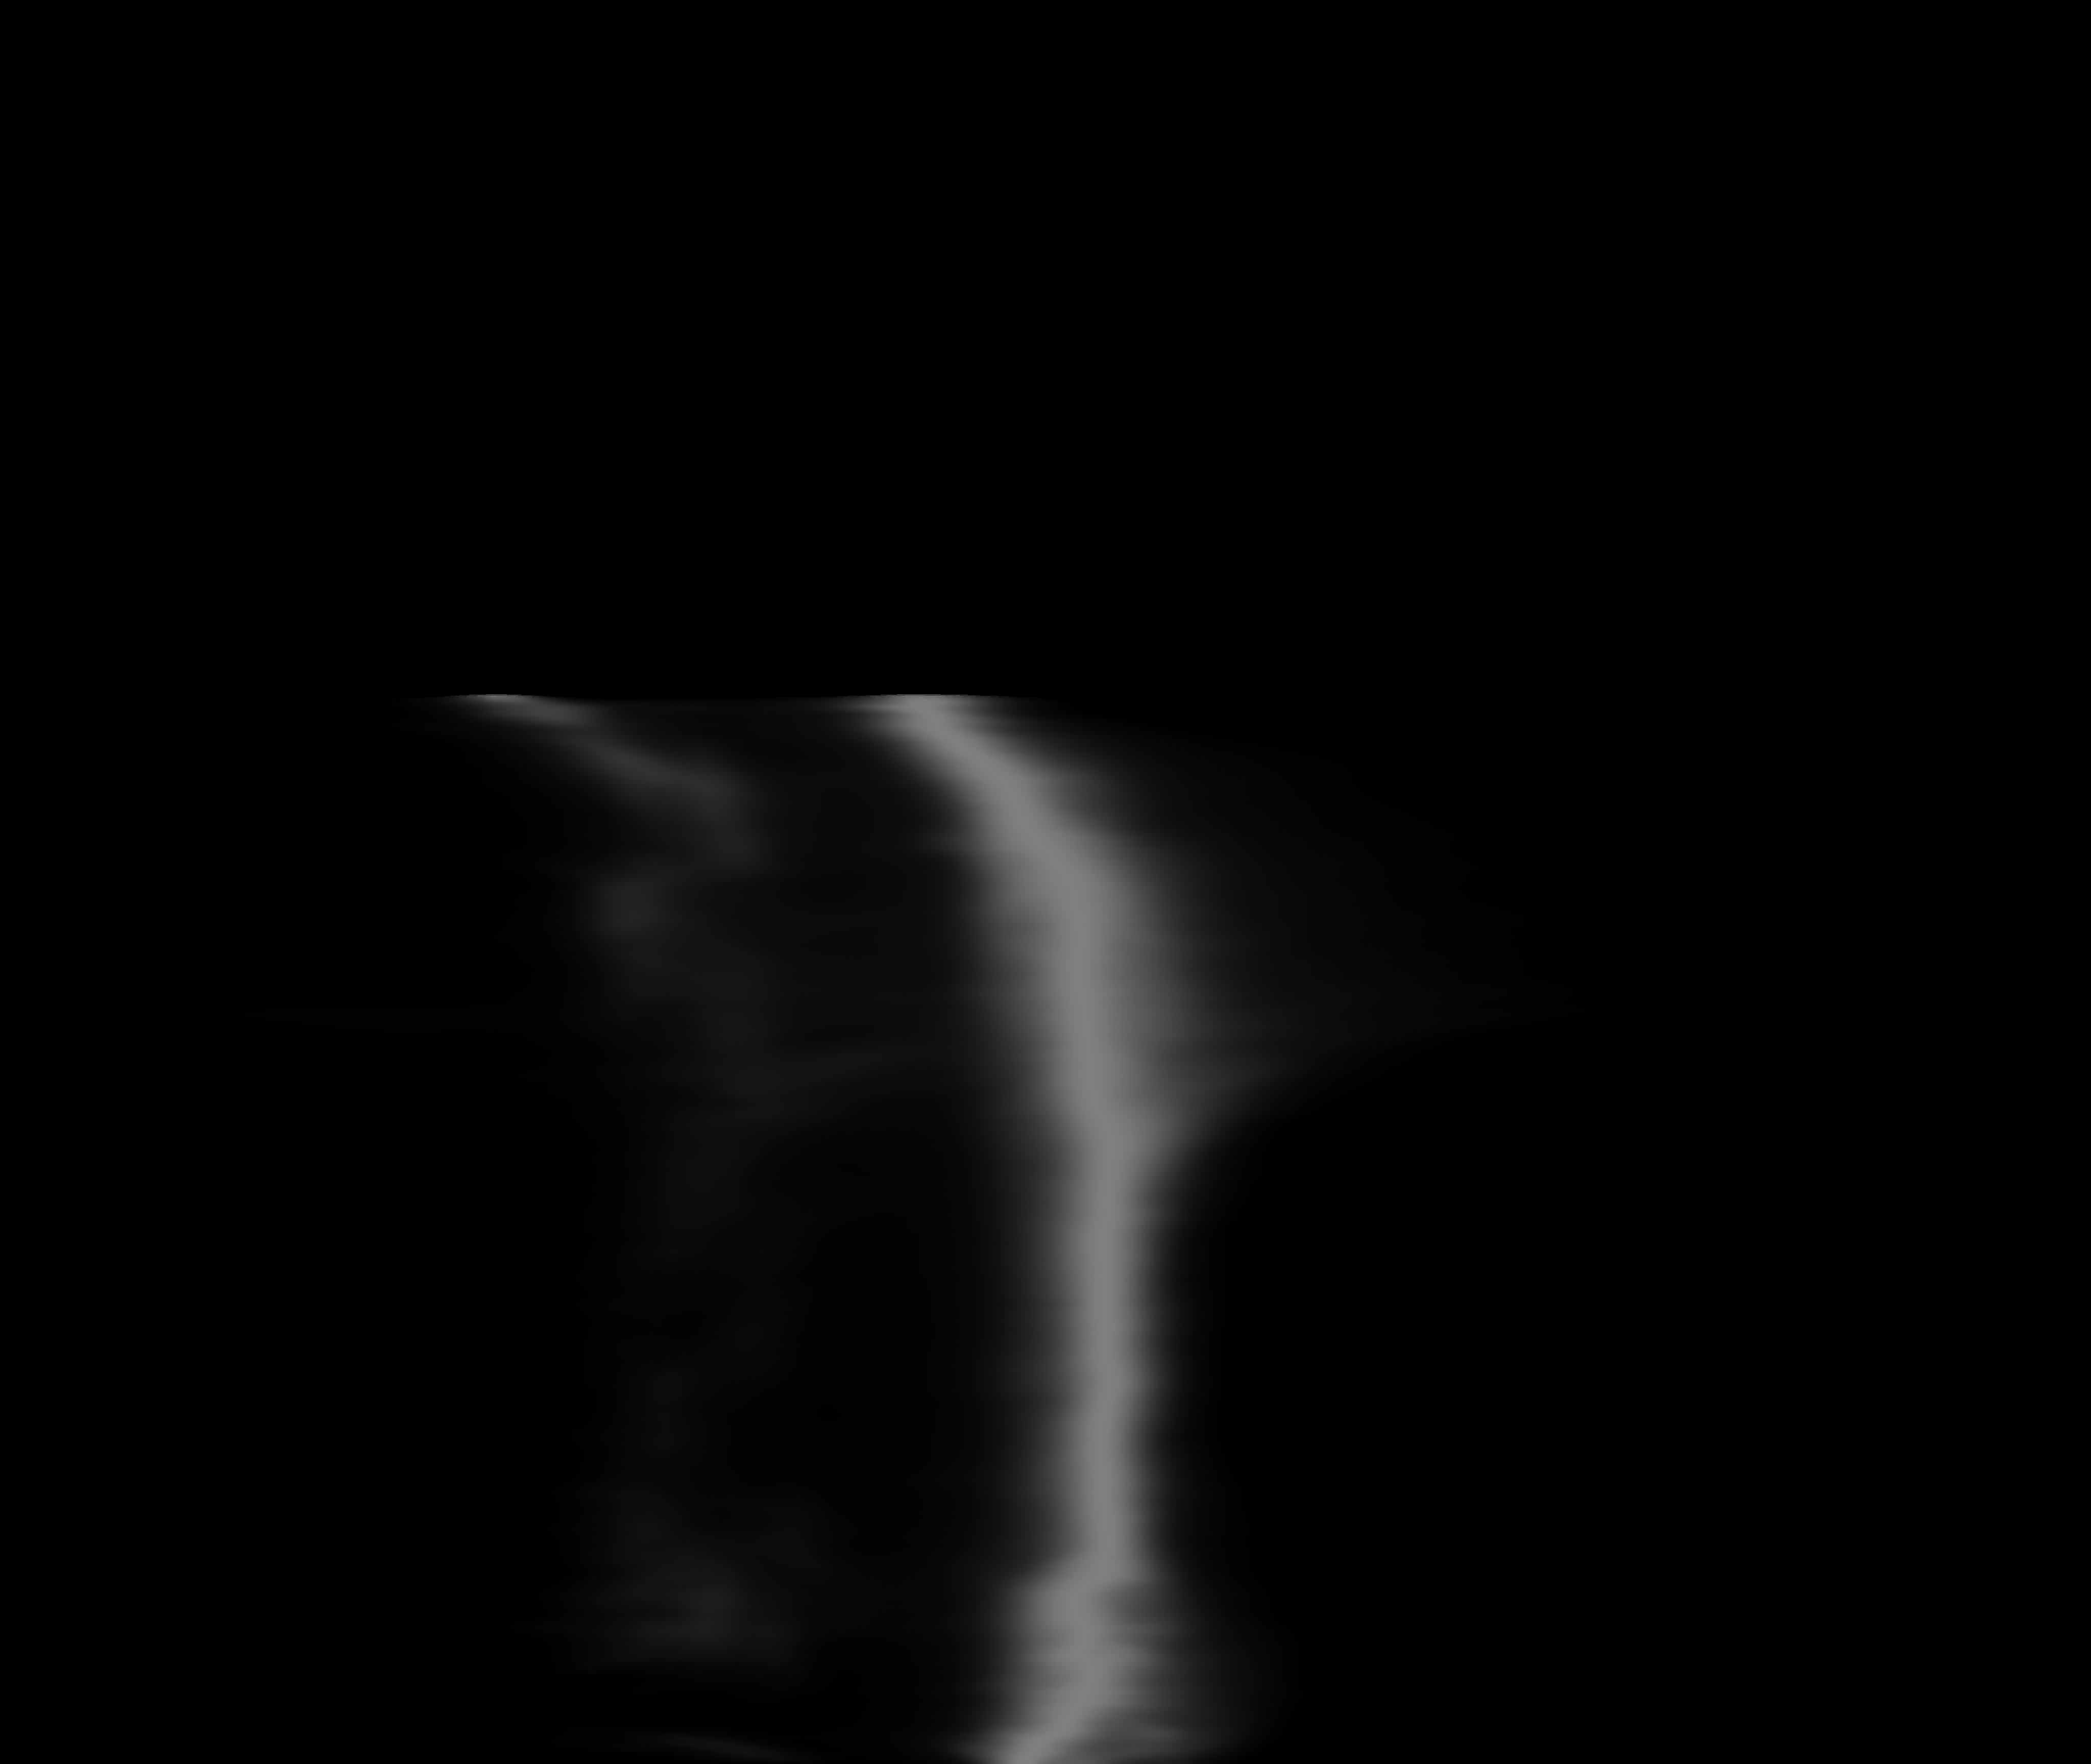
\includegraphics[width=.49\linewidth]{yb-bone_region3.png}
    %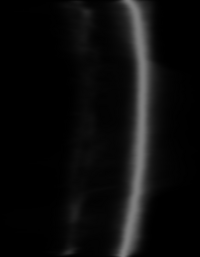
\includegraphics[width=.49\linewidth]{xb-bone_region3.png}
    %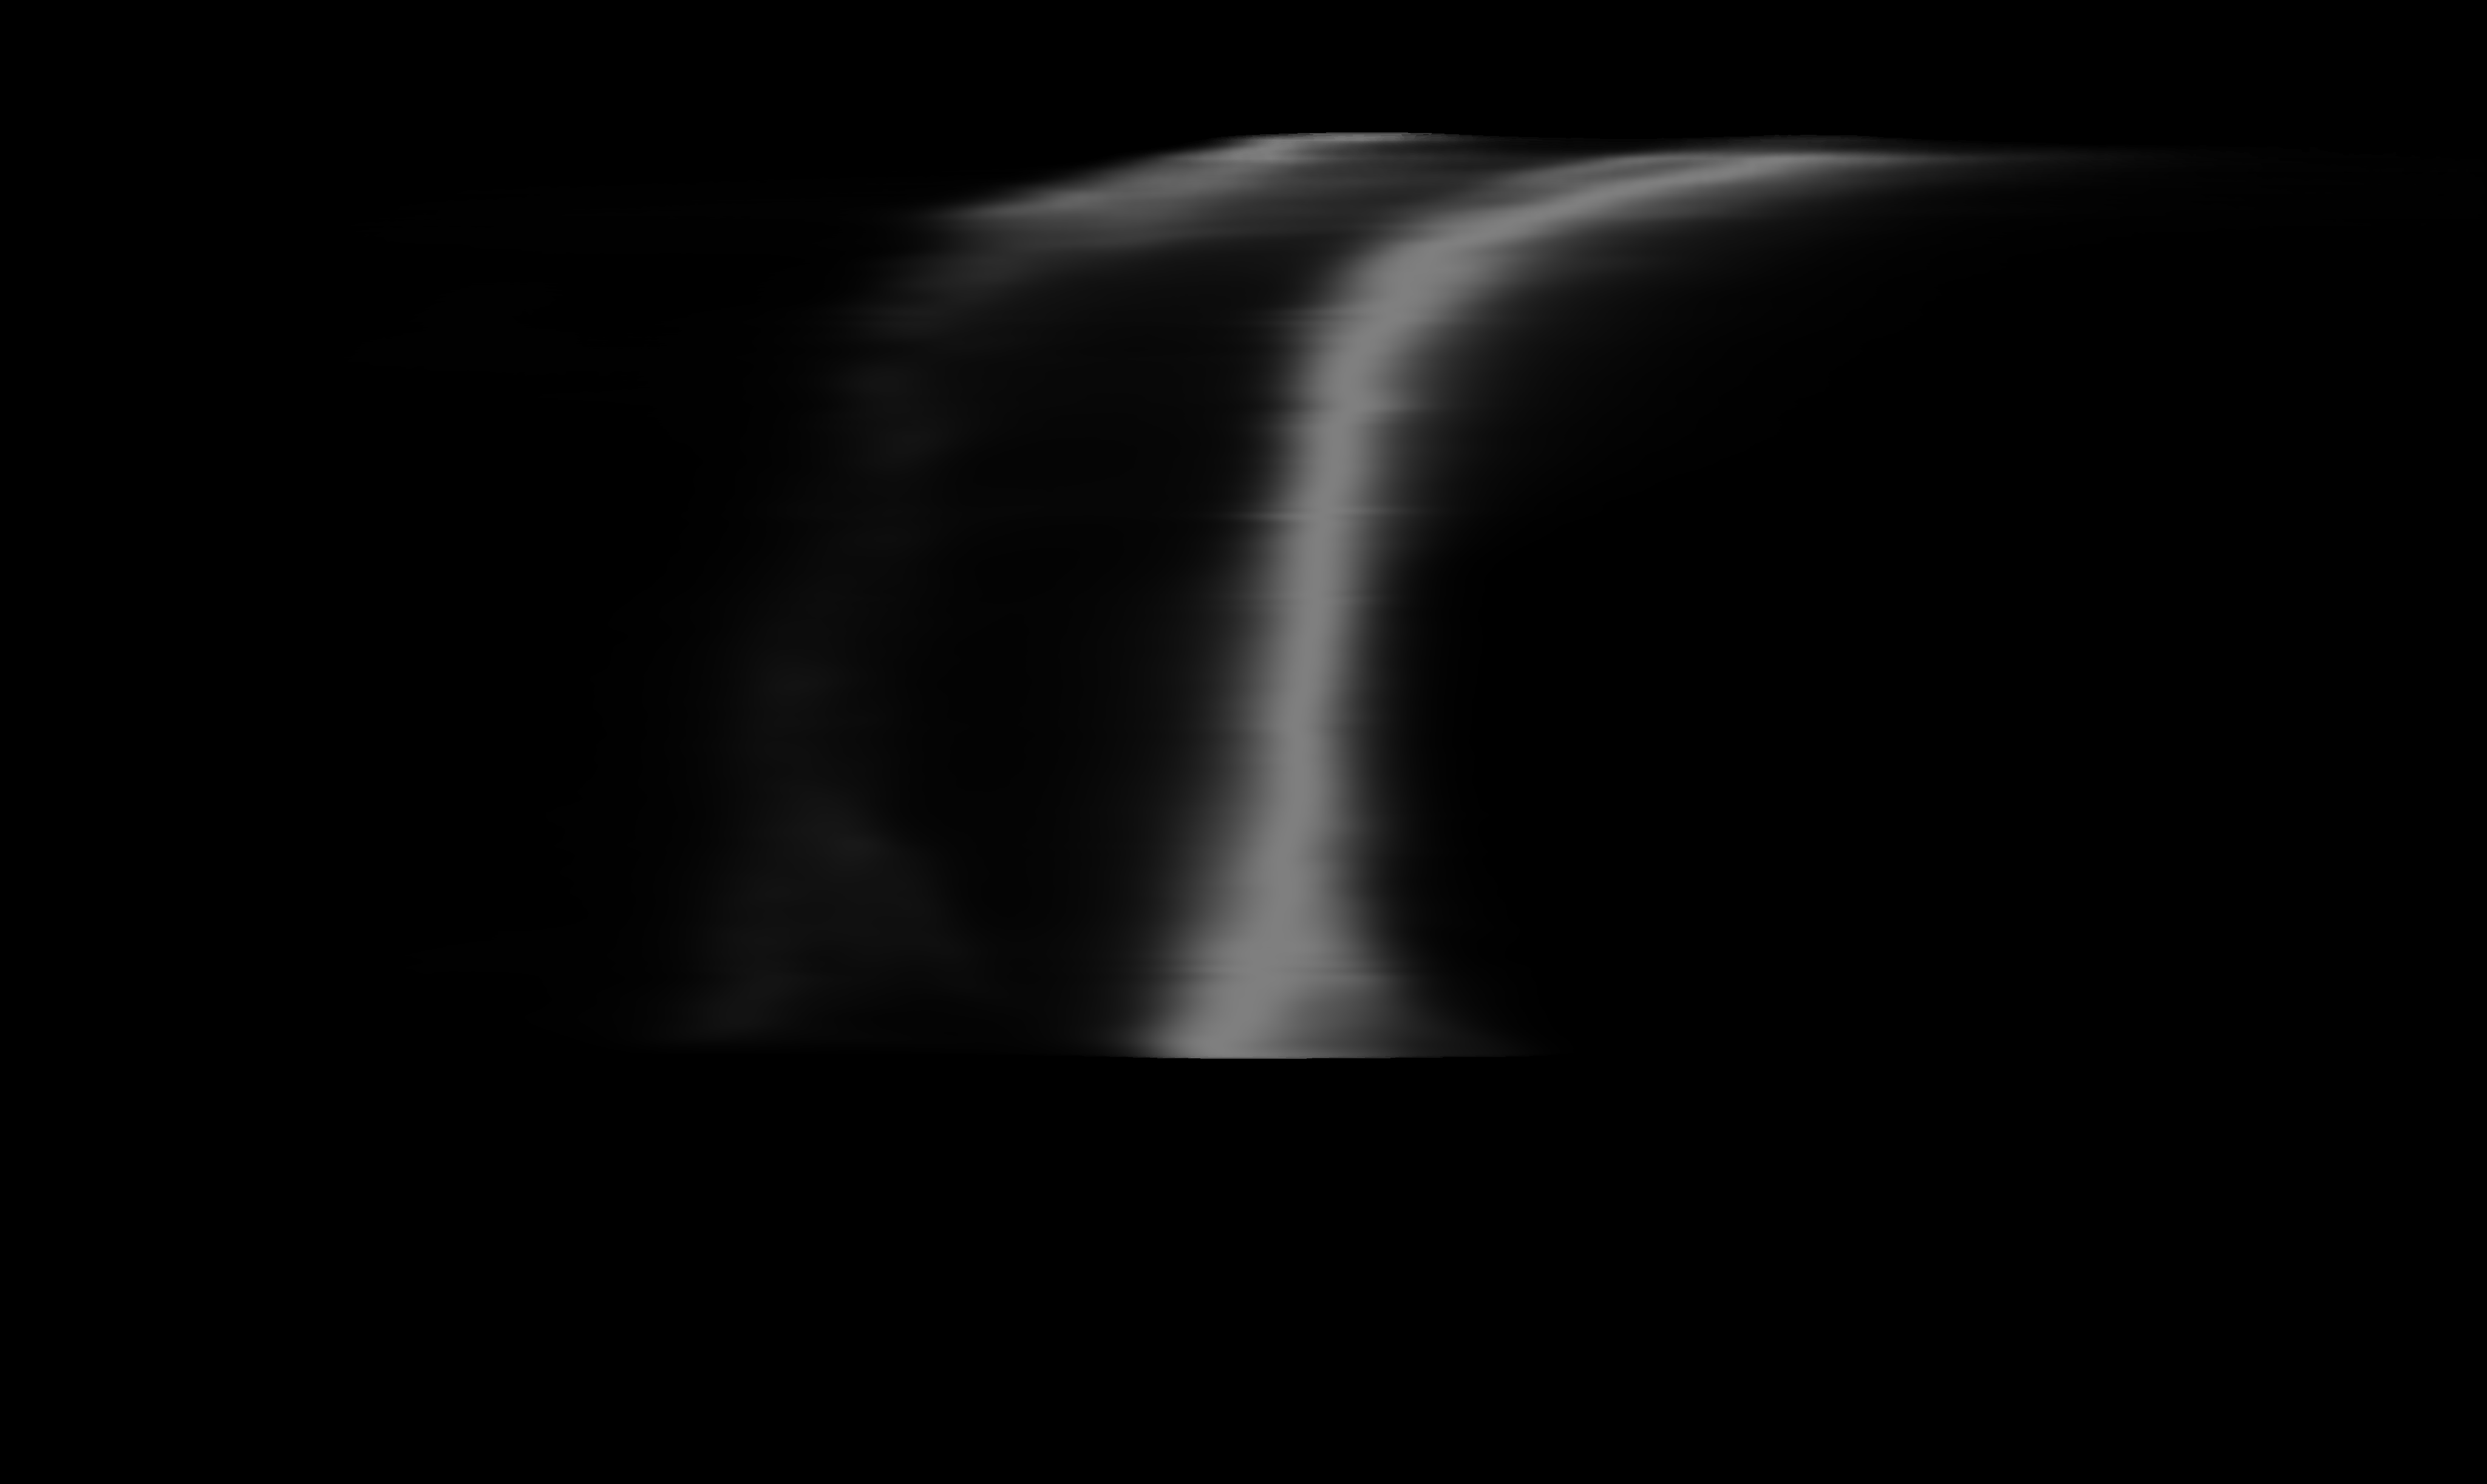
\includegraphics[width=\linewidth]{rb-bone_region3.png}
    \begin{tabular}{cc}
      \!\!\!\!\!\!(a) \begin{tabular}{c}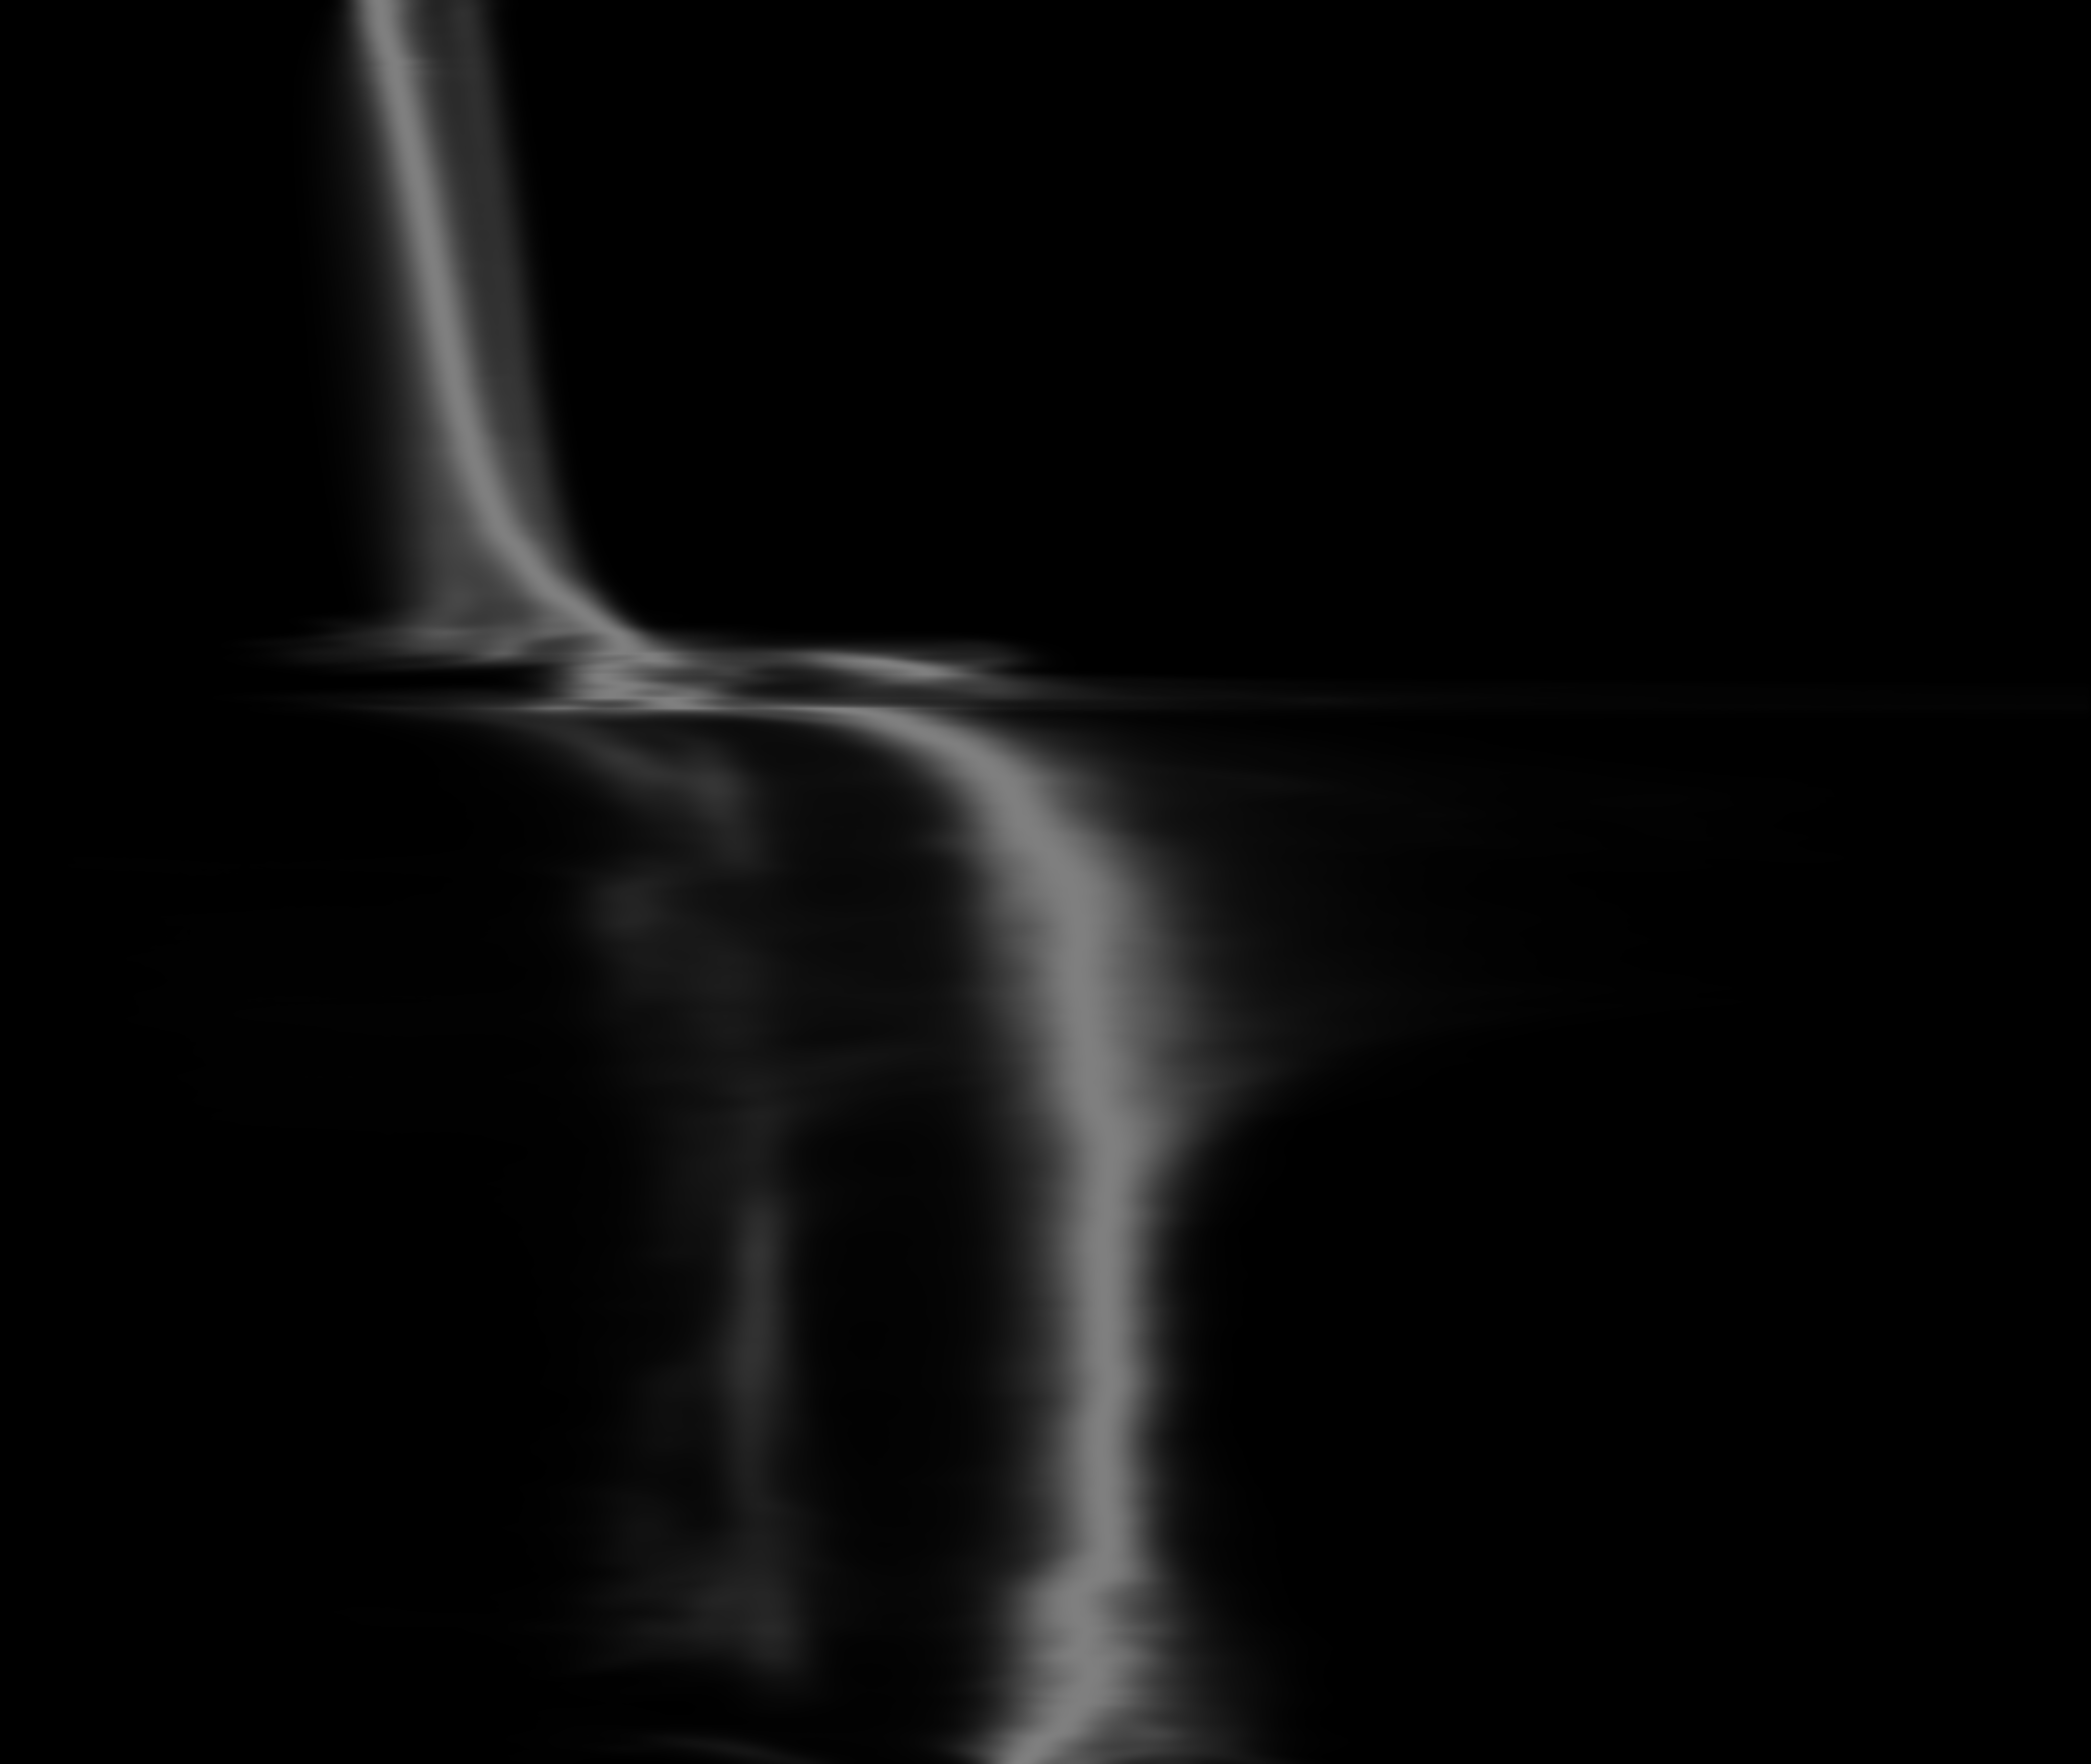
\includegraphics[width=0.7\columnwidth]{yb-full3.png}\end{tabular}\\
      \!\!\!\!\!\!(b) \begin{tabular}{c}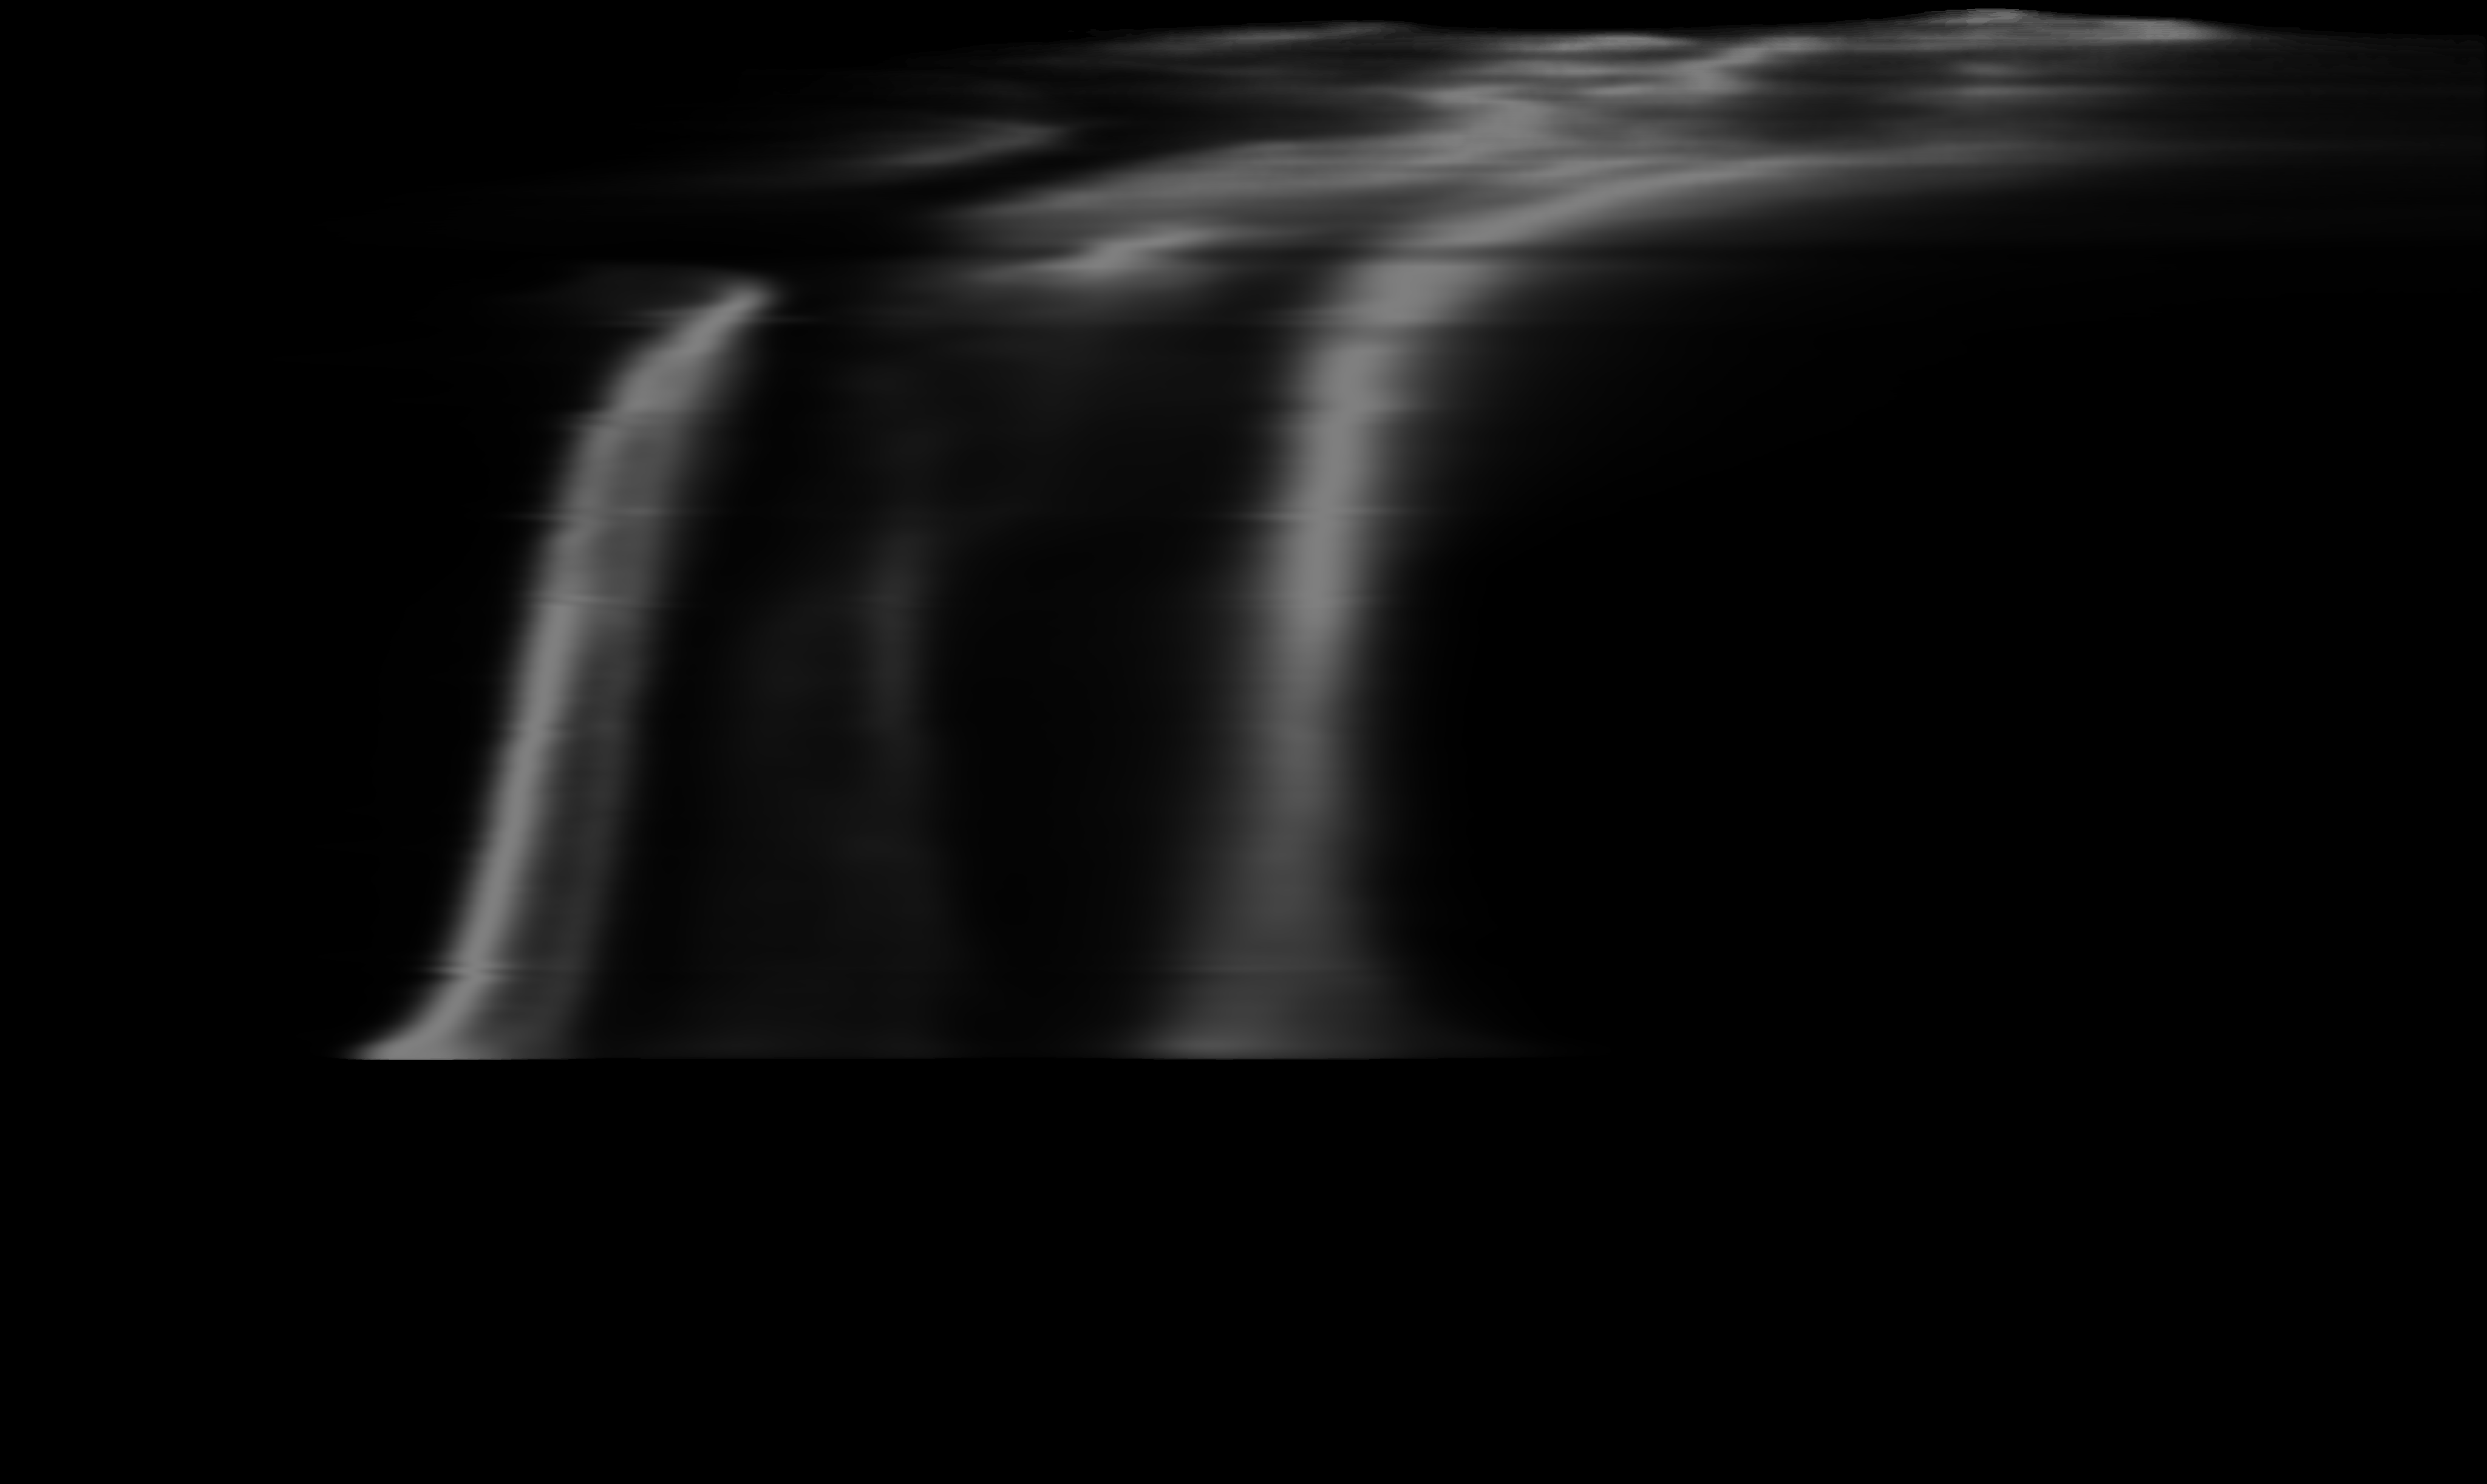
\includegraphics[width=0.7\columnwidth]{rb-full3.png}\end{tabular}\\
      \!\!\!\!\!\!(c) \begin{tabular}{c}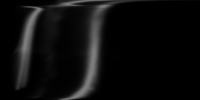
\includegraphics[width=0.7\columnwidth]{fb-edt-full2.png}\end{tabular}\\                        
%      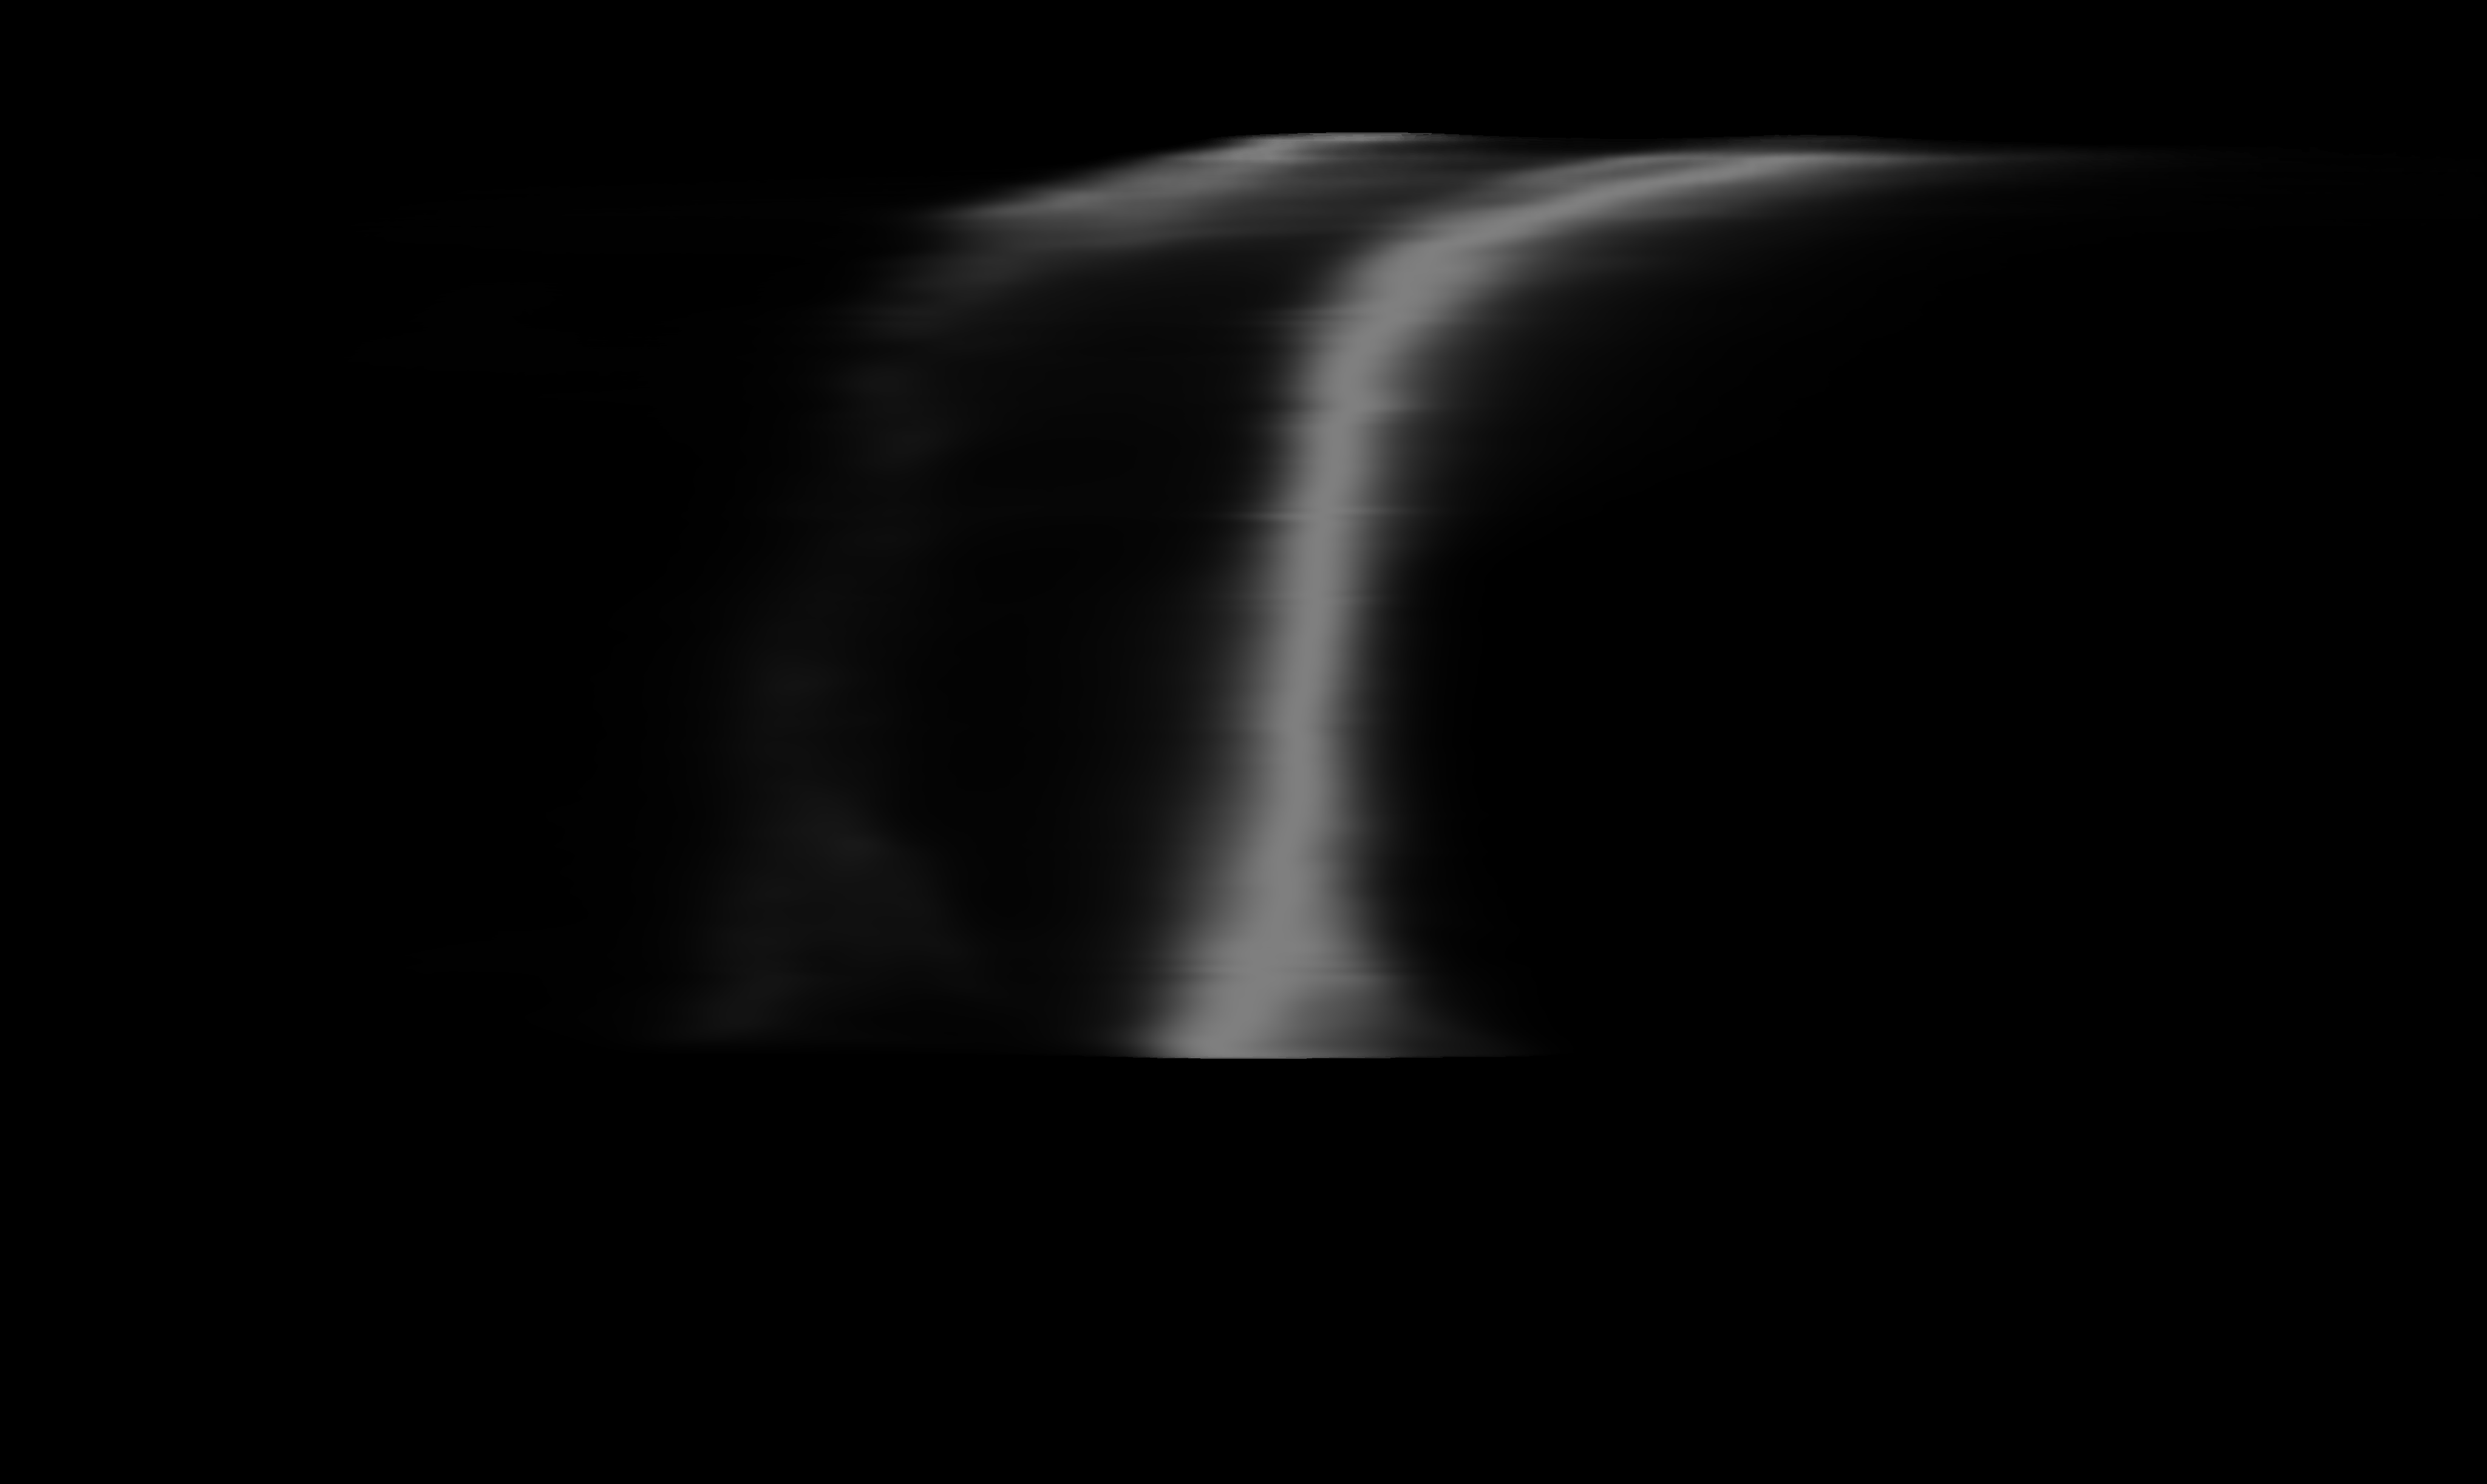
\includegraphics[width=\linewidth]{rb-bone_region3.png}\\      
    \end{tabular}
    \caption{Examples of 2D histograms for the full tomogram: (a) along the $y$-axis, (b) as a function of
      distance $r$ to the center, and (c) as a function of distance $d$ to the implant. The abscissa of the 2D histograms is voxel value, the ordinate is the value
      of $y$ resp.~$r$ and $d$. Notice that the $r$-2D histogram well separates the materials for large
      and intermediate values of $r$, but breaks down for small $r$. However, it clearly shows a brightening
      trend for small $r$. 
    }

    \label{fig:2dhists}
\end{figure}

\subsection{Field histograms}
%Show that the fields can perfectly separate
%discuss all the way to implant contact
In the present work, the main distortion we want to invert is the brightening of voxels near the high-contrast interface between
titanium implant and biological tissue, in order to accurately determine tissue-implant contact.
To this end, we can group the voxels according to their distance to the implant using the
{\em Euclidean Distance Transform} (EDT). \Cref{fig:2dhists}(c) shows the corresponding 2D histogram, which shows a darkening effect for large distances
(near the sample surface) and brightening for small distances (near the implant surface).

%EDT is good overall, but difficult close to the implant.
However, we can do better: As discussed in~\Cref{sec:physics}, the implant produces a \textit{glowing} effect, which
can be modeled physically by diffusion. \Cref{fig:edt-vs-diffusion} shows
how a voxel inside the troughs of the threading receives brightening contributions from many sides, while a voxel above the peak of the threading at
the same distance from the implant receives much less. To resolve brightening of voxels very close to the implant, it thus makes sense
to use a diffusion field, as shown in \Cref{fig:field-slice}. 


%TODO: Figuren er forkert (blå pile viser ikke afstand).
\begin{figure}
    \centering
    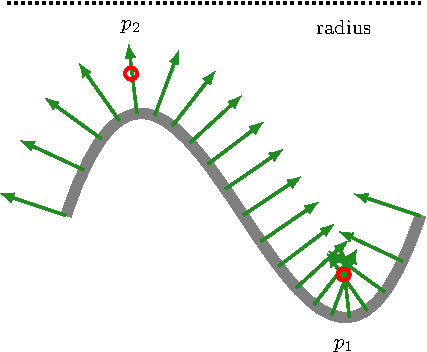
\includegraphics{glowing-crop}
    \caption{Visualization of glowing effect close to the implant surface, shown in the YZ plane. 
        The two points $p_1$ and $p_2$, marked in red, have the same distance to the implant, but receive markedly different brightening effect.
        Diffusion is depicted in green, where we see multiple arrows contributing to the value of $p_1$. The dotted line depicts a constant radius from the tomogram center.}
    \label{fig:edt-vs-diffusion}
\end{figure}


\begin{figure}
    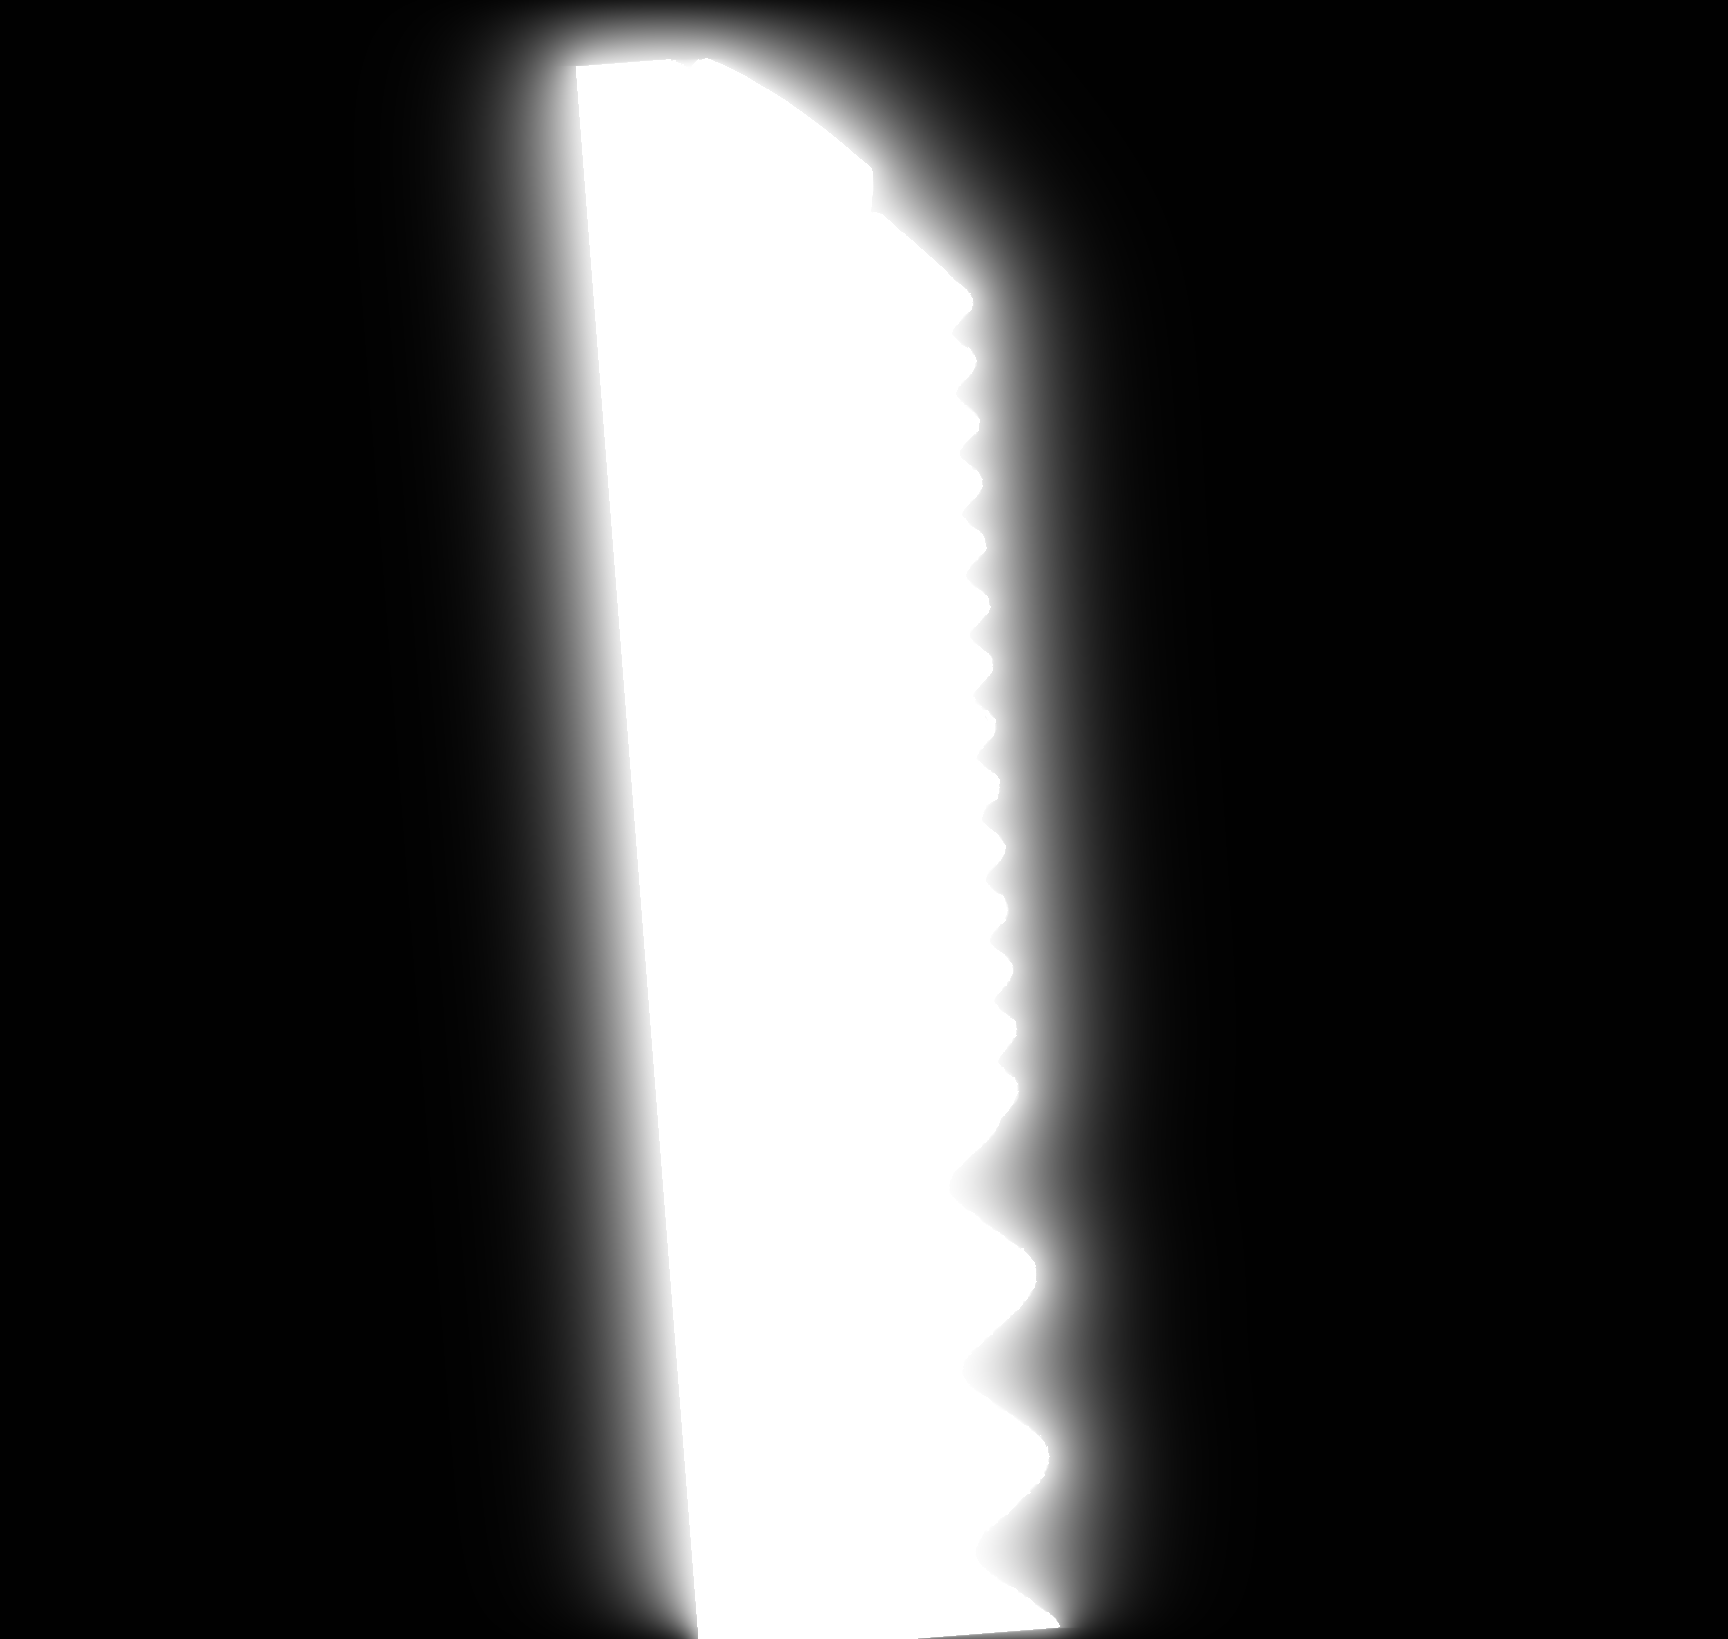
\includegraphics[width=\linewidth]{770c_pag-gauss-yz.png}
    \caption{A slice of the diffusion field in the YZ plane.}
    \label{fig:field-slice}
\end{figure}

Using a diffusion field to model the glow from the implant, we are able to describe the brightening effect even very close to the implant, but the field is nearly
zero everywhere else. In order
to construct a single field that separates voxels well according to the major contributions of distortion, we construct a combined EDT+diffusion field. We will see
in the next section that this is enough to produce a high-quality segmentation throughout the tomogram, both near the implant surface and far away from it.


% Show that the distance to the implant in edt will be the same in the grooves of the screw compared
% to the threads of the screw. This is "fixed" with diffusion, as the grooves will be brighter as it
% is surrounded by more implant.

%TODO: Adskil METODE, altsaa SASS, fra ANVENDELSE, altsaa BIC. 
\subsection{Walk-through of the method}
This section will describe each step of our method in detail. Going from tomography to a segmented tomography.

\subsubsection{Overview}
%Coarse steps, explain the idea
In order to reach the tissue-bone implant contact metric, we have the three coarse steps: compute the fields, segmentation using the fields, and extraction of the contact from the segmented tomography.
%
The steps of the field computation are:
\begin{enumerate}
    \item Compute the EDT and Diffusion fields to give each voxel spatial information about its relation to the implant.
    \item Compute frequency distributions of voxel values as functions of field values as 2D histograms.
\end{enumerate}
%    
Then, in order to segment using the fields:
\begin{enumerate}
    \item[3] Find the material ridges within the 2D histograms, using image processing techniques.
    \item[4] From the ridges, compute initial approximate frequency distributions of each material, which are then optimized to fit the 2D histograms.
          From the optimized distributions, we derive probability distributions for material classification. These distributions approximate the conditional probabilities $\Pof{m}{v,x}$ that a particular voxel belongs to material $m$ given that it has voxel value $v$ and field value $x$.
    \item[5] Apply the probability distributions to the tomography, segmenting the voxels into the different materials.
\end{enumerate}
%   
In the present paper, we use the improved segmentation to evaluate bone-implant contact and blood-implant contact.
\begin{enumerate}
\item[6] From the segmented tomography, we compute the network of blood vessels and the osteocyte network. Voxels are classified as bone, if they are in a connected component of bone-mineral and within a maximal distance from blood supply and osteocytes.
\item[7] Perform the tissue-to-implant contact analysis.
\end{enumerate}
%
These steps are also summarized in the flow chart in~\Cref{fig:flowchart}.

\begin{figure}
  \centering
  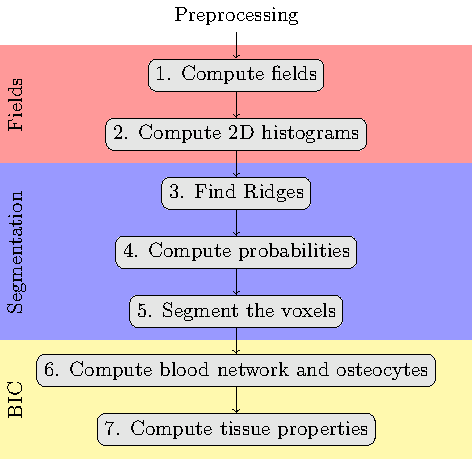
\includegraphics{steps}
    \caption{Flowchart depicting the steps of the method.}
    \label{fig:flowchart}
\end{figure}

\subsubsection{Segmentation}
The overall segmentation is computed in steps 1-5. For each step we will describe the process, showing
the algorithm where applicable, along with the the intermediate results.

\vspace{\baselineskip}
\noindent\textit{\textbf{Step 1: Field computations}}\\
Both fields are computed from the implant mask, as described in~\Cref{sec:preprocess}.
EDT is computed in parallel using W.~Silversmith's implementation of Meijster's algorithm \cite{pypi-edt},
% the Python package \texttt{edt}~\cite{pypi-edt}. %Den er implementeret i C++
yielding a 3D image in which every non-implant voxel is the Euclidean distance to the nearest implant voxel.

For diffusion, rather than solving a full diffusion equation, we approximate it using repeated convolutions
of a 3D-Gaussian kernel, implemented by separating into 1D convolutions, as seen in~\Cref{alg:diffusion}, and the XZ-plane in~\Cref{fig:field-slice}.

\begin{algorithm}
    \caption{Diffusion approximation.}
    \label{alg:diffusion}
    \begin{algorithmic}
        \Function {Diffusion} {$|voxels|[n_z*n_y*n_x]$, $repetitions$, \newline \indent \indent $|kernel|[2*k+1]$}
            \State $S \gets [n_y * n_x, n_x, 1]$
            \State $N \gets [n_z, n_y, n_x]$
            \State $|buf|_0[:] \gets |voxels|[:]$
            \For {$rep$ \textbf{in} $repetitions$}
                \For {$dim$ \textbf{in} $dimensions$}
                    \For {$z,y,x$ \textbf{in} $0{:}n_z,0{:}n_y,0{:}n_x$}
                        \State $X \gets [z,y,x]$
                        \State $i_{start} \gets - \min (k, X[dim])$
                        \State $i_{end} \gets \min (k, N[dim] - X[dim] - 1)$
                        \State $i_{global} \gets z*S[0] + y*S[1] + x*S[2]$
                        \For {$i$ \textbf{in} $i_{start}:i_{end}$}
                            \State $i_\text{offset} \gets i_\text{global} + i*S[dim]$
                            \State $|buf|_1[index] \gets |buf|_0[i_\text{offset}] * kernel[i+k]$
                        \EndFor
                    \EndFor
                    \State $|buf|_0[:] \gets |buf|_1[:]$
                \EndFor
               \EndFor\\
            \Return $|buf|_0$
        \EndFunction
    \end{algorithmic}
\end{algorithm}

%EDT + Diffusion
To obtain a good separation both close to the implant and far away, we combine the two fields into a
single one as shown in~\Cref{eq:field-comb}.

%\begin{algorithm}
%    \caption{Field combination}
%    \label{alg:field-comb}
%    \begin{algorithmic}
%        \Function {field\_combine} {$f_{edt}, f_{dif}$}
%            \State $r \gets f_{dif} - \frac{f_{edt}}{\max (f_{edt})}$
%            \State $r \gets r - \min (f_{dif})$
%            \State $r \gets \frac{r}{\max (f_{dif})}$
%
%            \Return $r$
%        \EndFunction
%    \end{algorithmic}
%\end{algorithm}

\begin{equation}
    \label{eq:field-comb}
    \begin{split}
        f_{combined} &= \frac{f_{diffusion} - \frac{f_{edt}}{\max (f_{edt})} \min (f_{diffusion})}{\max (f_{diffusion})}
    \end{split}
\end{equation}

\vspace{\baselineskip}
\noindent\textbf{Step 2: 2D histograms} \\
From the combined fields we compute a 2D-histogram with the field value on the y-axis and the voxel
value on the x-axis.  The algorithm for the field-histogram can be seen in~\Cref{alg:field-hist}
along with a plot of the resulting histogram in~\Cref{fig:field-hist}. We see that the bone and soft tissue
separate neatly into two distinguishable distributions. The effect of the diffusion field is to ``zoom in'' near the implant surface,
where the diffusion field changes rapidly.


\begin{algorithm}
    \caption{Field 2D histograms.}
    \label{alg:field-hist}
    \begin{algorithmic}
        \Function {Field\_hist} {$|voxels|[n_z,n_y,n_x]$, $\field[n_z,n_y,n_x]$, $v_{bins}$, $v_{min}$, $v_{max}$, $f_{bins}$, $f_{min}$, $f_{max}$}
            \For {$z,y,x$ \textbf{in} $0{:}n_z,0{:}n_y,0{:}n_x$}
                \State $v \gets |voxels|[z,y,x]$
                \If {$v_{min} \leq v \leq v_{max}$}
                    \State $f \gets |voxels|[z,y,x]$
                    \If {$f_{min} \leq f \leq f_{max}$}
                        \State $v_i \gets (v_{bins} - 1) - \frac{v - v_{min}}{v_{max} - v_{min}}$
                        \State $f_i \gets (f_{bins} - 1) - \frac{f - f_{min}}{f_{max} - f_{min}}$
                        \State $h[f_i,v_i]{+}{+}$
                    \EndIf
                \EndIf
            \EndFor
            \Return $h$
        \EndFunction
    \end{algorithmic}
\end{algorithm}

\begin{figure}
    %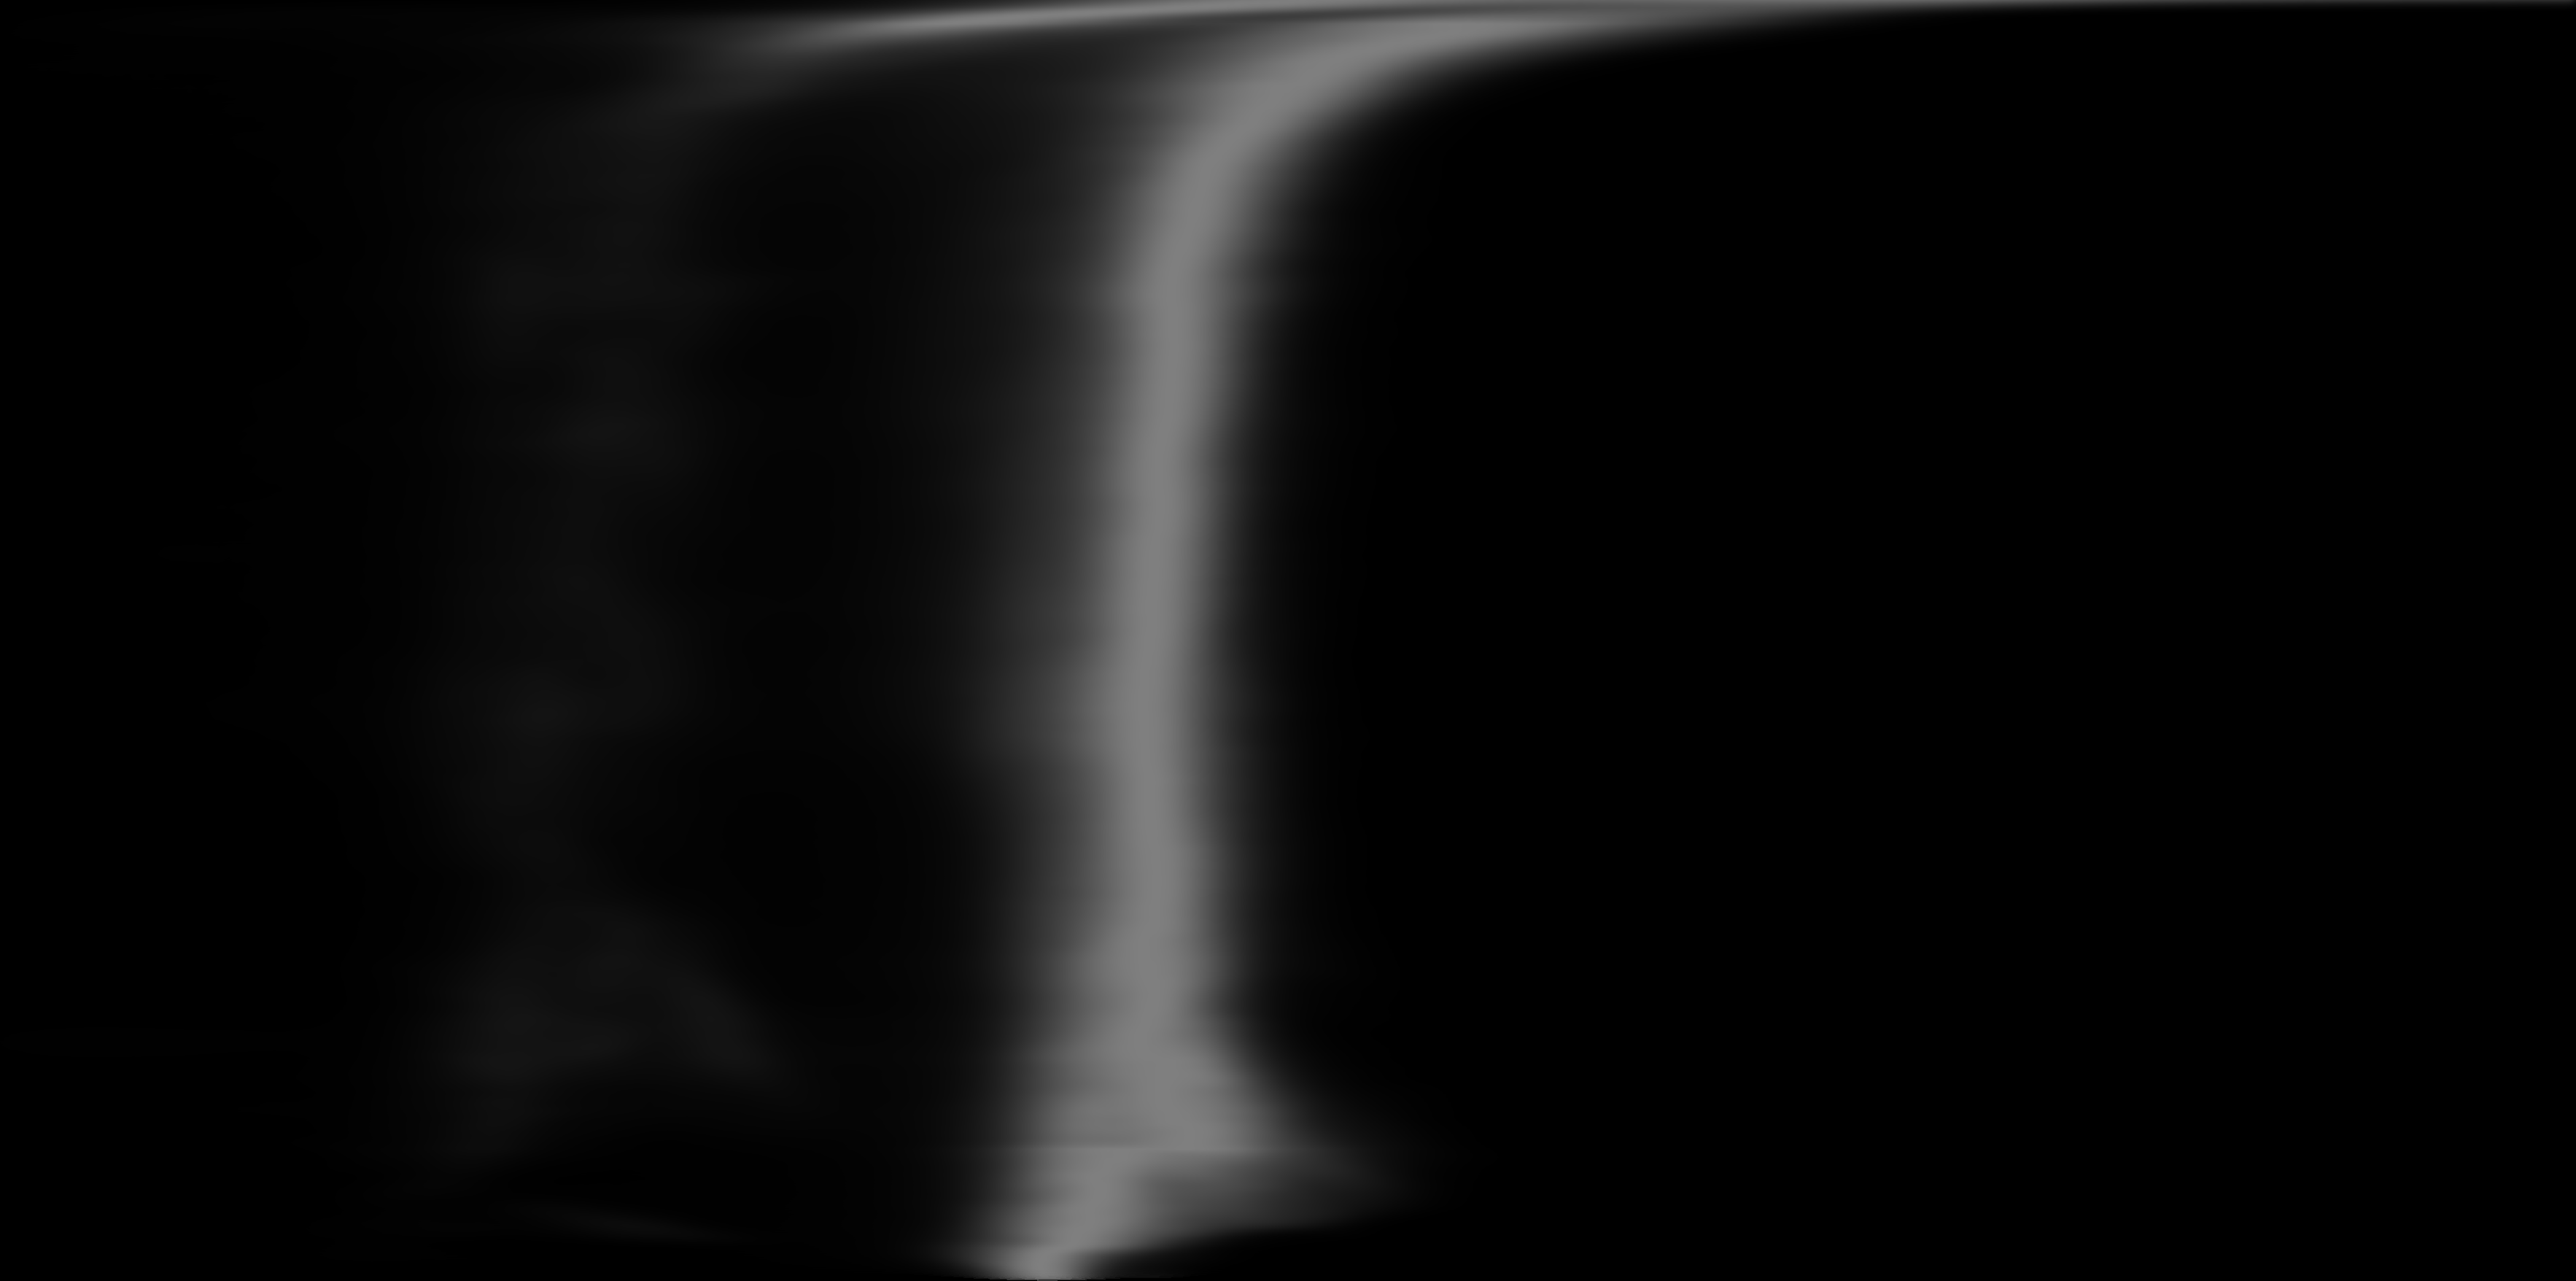
\includegraphics[width=\linewidth]{fb-edt-bone_region3.png}
    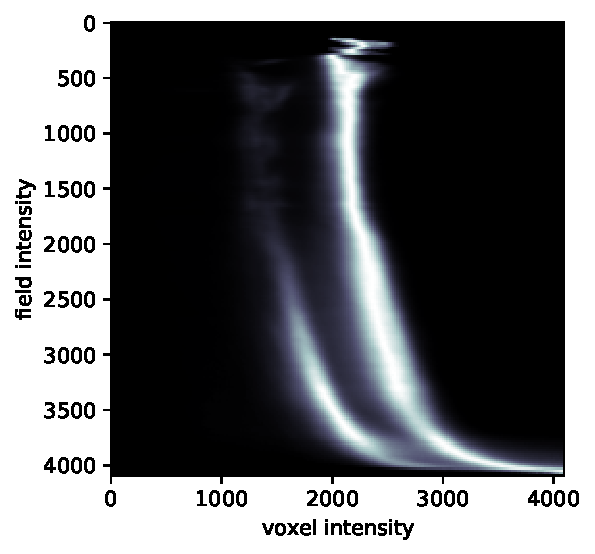
\includegraphics[width=\linewidth]{fb-gauss+edt-bone_region3.pdf}
    \caption{2D field histogram. Note that there are two clearly separated ridges, which each represent
      the expectation value for a particular material as a function of the field value.}
    \label{fig:field-hist}
\end{figure}

\vspace{\baselineskip}
\noindent\textbf{Step 3: Identify the materials} \\
In order to decompose 2D histogram into a sum of probability distributions that represent
the different materials present in the tomogram, we first identify the {\em ridges}:
i.e., the peaks in the 1D histograms that are persistent and vary continuously with the field value.
Thus we can expect each ridge to represent the {\em expectation values} for a particular material
as a function of the field value, i.e., as a function of the voxel's position in space.
%
Any ridge-finding method will do: we compute it through the series of image processing operations shown in
\Cref{alg:material}.
% The next step is to isolate the different materials spatially, which is done through the field-histogram.
% For our first attempt, we applied Otsu's threshold to each each row in the 2D-histogram. While this
% provided good results for two well defined distributions, it eventually began to fail. This was either
% because of lack of samples, or because the histogram did not contain two distributions, which is an
% underlying assumption of Otsu thresholding. These two effects occurred at the edges (both closest and
% furthest from implant), which would bleed into the later steps of the segmentation process.

% Rather than finding the threshold value in between the distributions, our next solution was to start
% finding the distributions by finding the ridges of the 2D-histogram. We do this by applying a series
% of image processing techniques, described in~\Cref{alg:material}. Each of the resulting contours
% become their own material, which are then labeled as material 1 or 2 respectively for this particular
% sample. For samples that would contain more than two distributions, the same algorithm should apply,
% as long as the distributions does not overlap.

\begin{algorithm}
    \caption{2D histogram ridge-finding.}
    \label{alg:material}
    \begin{algorithmic}
        \Function {Ridges} {$h[f_{bins}$, $v_{bins}]$, $\sigma$, $peak_{min}$, $k_x$, $k_y$, \newline \indent \indent $i_{dilate}$,$i_{erode}$, $t$}
            \For {$row$ \textbf{in} $0{:}f_{bins}$}
                \State $r \gets |gaussian\_smooth|(h[row,:], \sigma)$
                \State $p \gets |find\_peaks|(r, peak_{min})$
                \State $ps[p] \gets 1$
            \EndFor
            \State $kernel = |cross\_kernel|(k_x, k_y)$
            \State $d \gets |dilate|(ps, i_{|dilate|}, kernel)$
            \State $e \gets |erode|(d, i_{|erode|}, kernel)$
            \State $cs \gets |find\_contours|(e)$
            \For {$i$ \textbf{in} $0{:}cs$}
                \If {$size(cs[i]) > t$}
                    \State $l \gets |draw\_contour|(l, cs[i], i+1)$
                \EndIf
            \EndFor\\
            \Return $l$
        \EndFunction
    \end{algorithmic}
\end{algorithm}

\begin{figure*}
    % %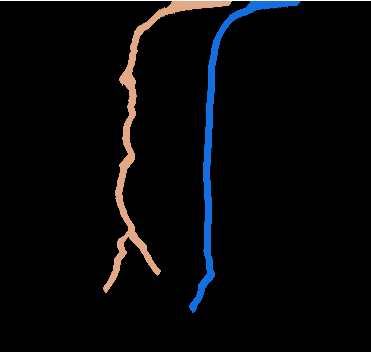
\includegraphics[width=0.5\linewidth]{curves_edt.png}%
    % %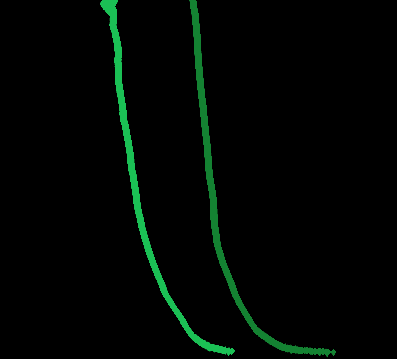
\includegraphics[width=0.5\linewidth]{curves_diffusion.png}
    % 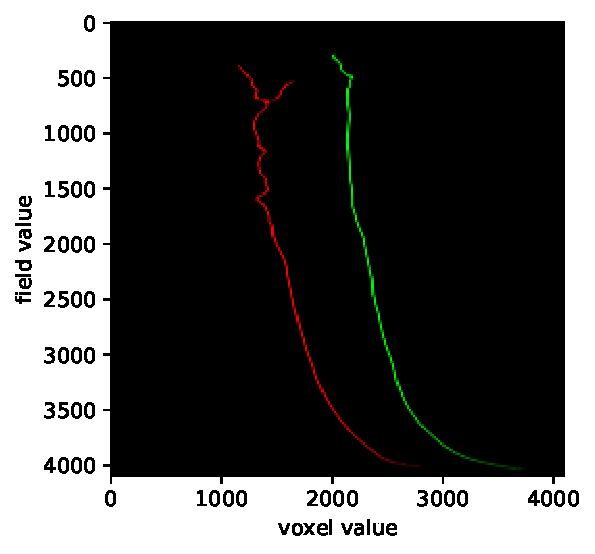
\includegraphics[width=\linewidth]{ridges_gauss+edt-bone_region3.pdf}
    % \james{will produce overall plot with probabilities}
    % \caption{Detected ridges from the combined field histogram.}
    % \label{fig:curves}
  \centering
  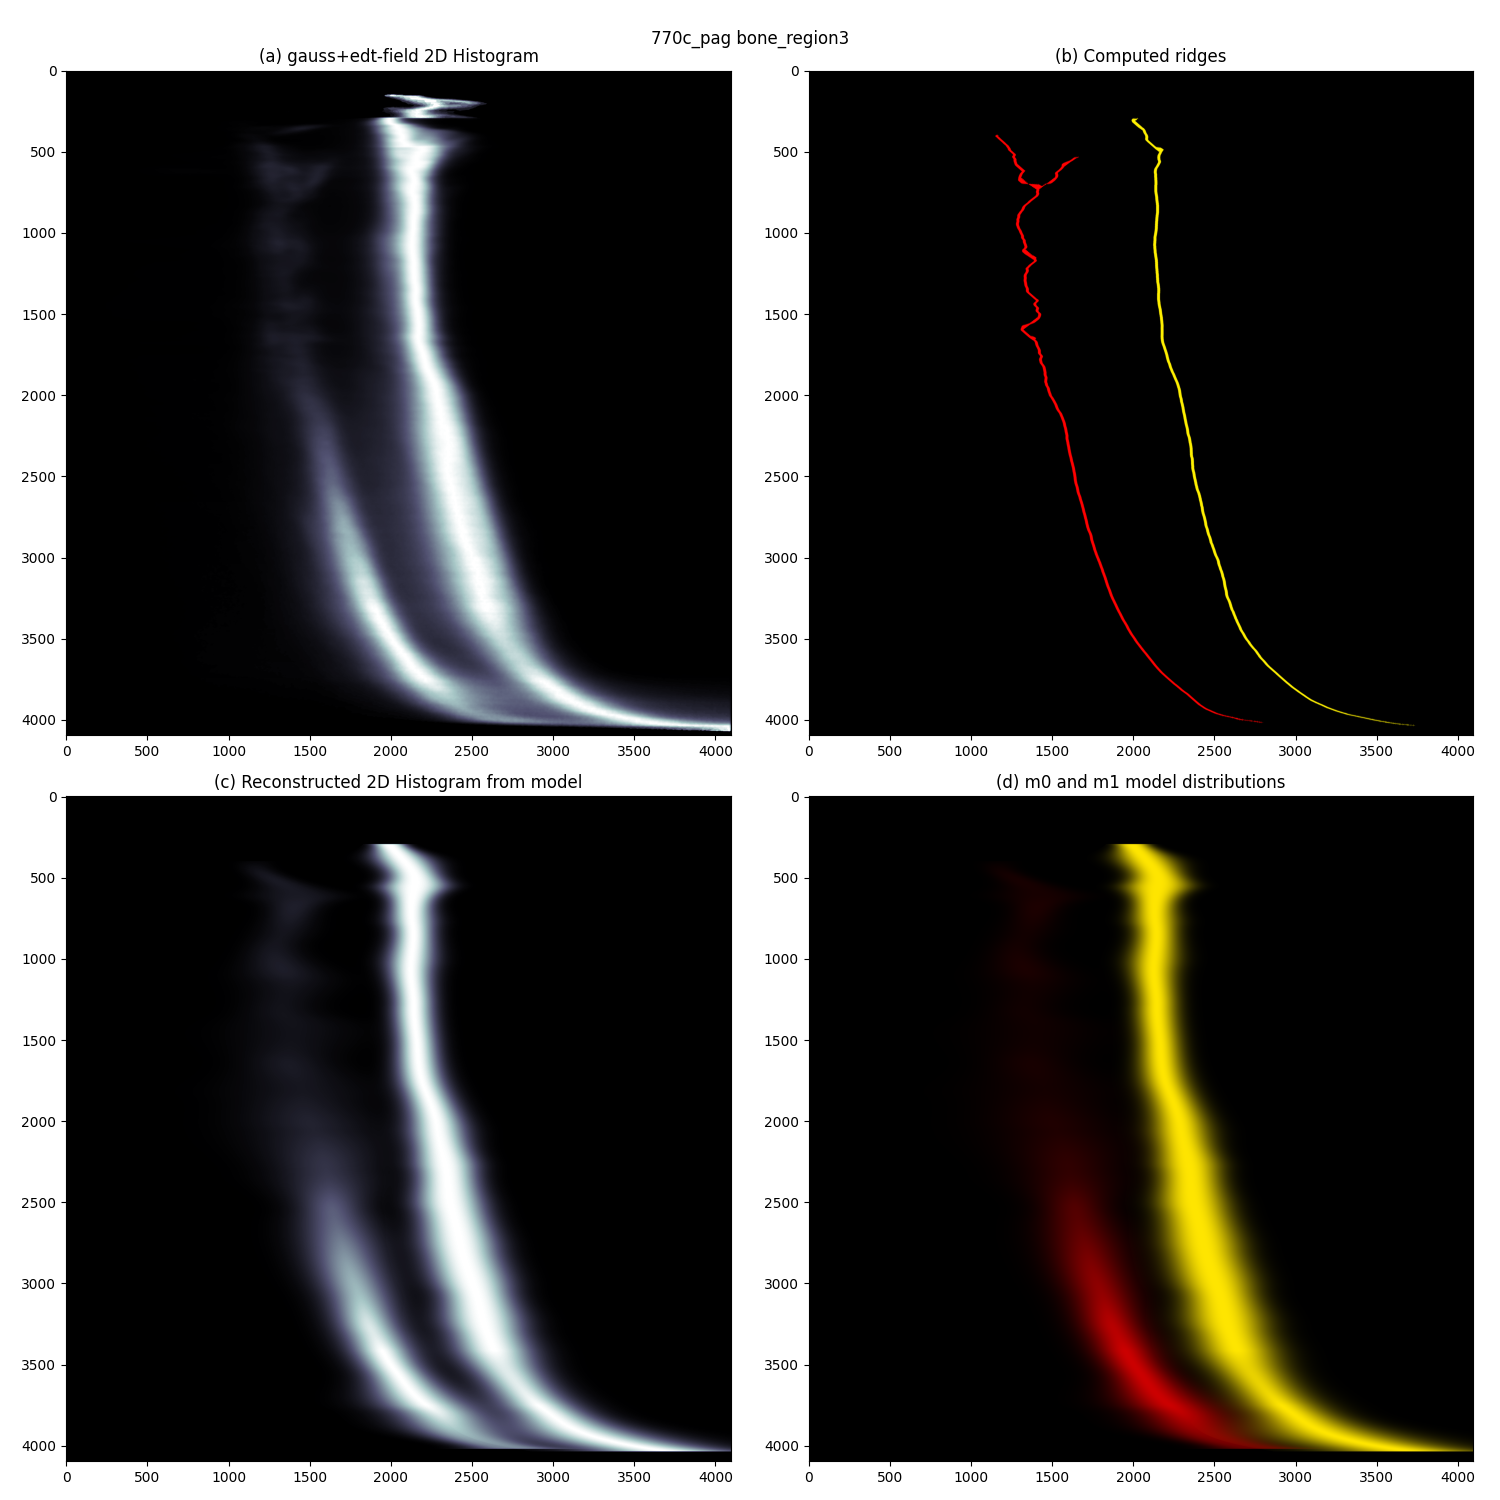
\includegraphics[width=.9\textwidth]{compute_probabilities_gauss+edt_bone_region3}\\
  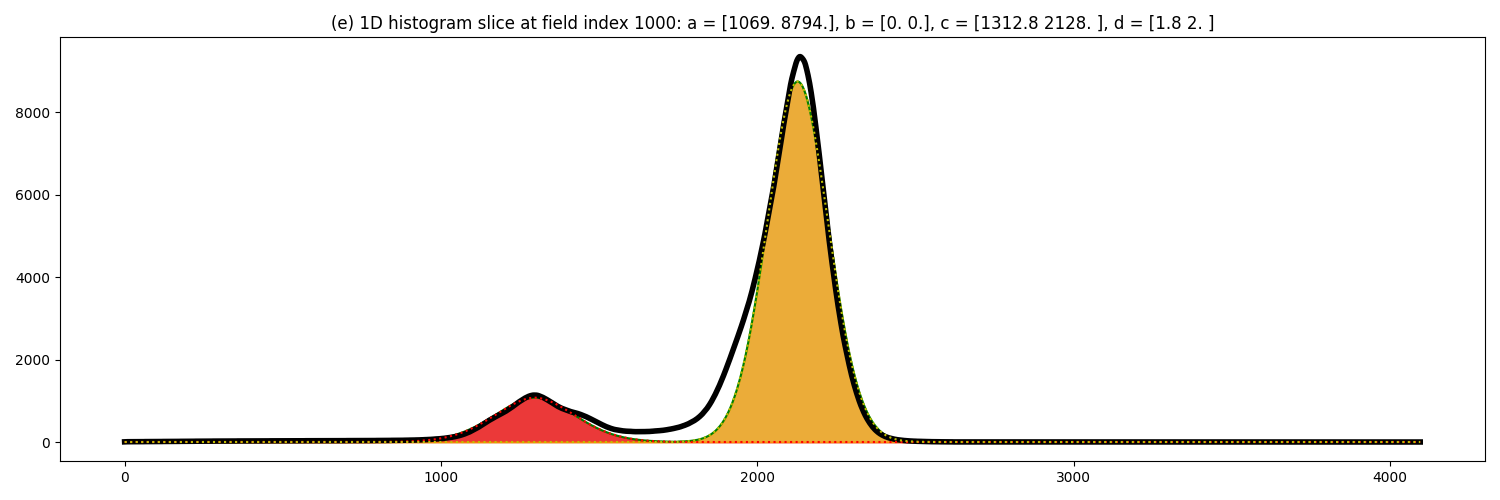
\includegraphics[width=.9\textwidth]{hist_slice_gauss+edt_bone_region3}\\
  \caption{(a) Measured 2D histogram for the compound diffusion+distance field from Step 2. (b)
    The detected ridges from Step 3. (c) Sum of computed frequency distribution models
    with optimized smooth piecewise cubic functions for parameters $a(\fval), b(\fval), c(\fval), d(\fval)$:
    this is the part of the 2D histogram explained by the smooth model. (d) The individual distributions evaluated
    on the 2D field-value$\times$ voxel-value grid. (e) A single 1D slice of the 2D histogram (black) together with
    the model frequency distributions. Red is soft-tissue, yellow is bone mineral.
  }
  \label{fig:curves-and-more}
\end{figure*}

\vspace{\baselineskip}
\noindent\textbf{Step 4: Compute models for material probability distributions} \\
Our goal is to obtain good conditional probability distributions $\Pof{m}{v,\xx}$
that model the likelihood of a voxel having material type $m$ as a function
both on its value $v$ and its position $\xx$ in space. For the probabilities
conditioned on the field values (distance or diffusion field), we model
the probability distributions $\Pof{m}{v,f(\xx)}$ conditioned on
voxel- and field values. We want to make sure that these distribution
functions vary smoothly across space (or as a function of field values),
to ensure that we can identify the materials correctly across the entire
image: i.e., even though the frequency distributions look completely different
close to the titanium implant compared to the middle region or sample surface,
we can track the unbroken, smooth deformation to assign a global material
identity.

To this end, we first {\it model the frequency distributions} using the
2D histograms. Given that we are modeling materials $m=1,\ldots,M$,
we write the full 2D histogram as a sum of distributions
$g_m(\fval,v)$ representing the modeled part, and a
residual $r(\xx,v)$.
\begin{equation}
  \label{eq:hist}
  H(\fval,v) = \sum_{m=1}^M g_m(\fval,v) + r(\fval,v)
\end{equation}
The residual is constrained to be non-negative, i.e., we must not explain
more voxels than the image contains.
The distribution functions can be chosen in any way that approximately
model the observed frequencies: we first used Gaussians with passable success,
but found that they dropped off too rapidly. We instead found excellent results
with the next-simplest model, leaving the exponential power $d_m(x)$ as a free parameter:
\begin{equation}
  \label{eq:dist-form}
  g_m(\fval,v) = a_m(\fval) e^{-b_m(\fval) \vert v-c_m(\fval)\vert^{d_m(\fval)}}
\end{equation}
In Eq.~\eqref{eq:dist-form}, each field value $\fval$
$a(\fval)$ is the distribution height at the center $v=c(\fval)$;
$b(\fval)$ is the exponential falloff rate; and $d(\fval)$ is
the exponential power ($d=2$ yields a Gaussian, $d=1$ a simple exponential).
In practice we found $1.5\le d \le 2$ to best match the actual frequency
distribution decay rates.

Using the ridges found in the previous step, we generate good starting
guesses and constraints for the distribution parameters
$a,b,c,d$:
For each field-value $\fval$ (corresponding to a row in the 2D histogram),
we initialize the starting approximation as:
\begin{equation}
  \label{eq:starting-guesses}
  \begin{array}{lll}
    c_m(\fval) &= \mathop{\mathtt{argmax}}_{v \text{ with }\lab[\fval,v] = m} H(\fval,v)  & \text{Peak position}  \\
    a_m(\fval) &= H(\fval,c_m(\fval)) & \text{Peak value}\\
    b_m(\fval) &= 3/\mathrm{width}_m(\fval)^2  & \text{Decay rate}\\
    d_m(\fval) &= 2 & \text{Exponential power}
  \end{array}
\end{equation}
where we use half the distance to the center of ridge $m+1$ as the width
$\mathrm{width_m}(\fval)$, using the relation that $b = 3/w^d$ yields
a $5\%$ cutoff at $w$ for any $1\le d \le 2$. This approximation
already yields a good approximation. Thus, the subsequent
optimization using the constrained quasi-Newton optimization method L-BFGS-B\cite{BFGS}
converges rapidly to an excellent fit. Each 1D histogram row is first optimized
independently in parallel: The resulting numerical functions
$a_m(\fval),\ldots,d_m(\fval)$ are then converted into piecewise cubic
functions using a least squares-based algorithm that ensures continuity
and differentiability across the piecewise segments. This lets us interpolate across
outliers due to noise, but equally important:
extrapolate our models smoothly into the regions very close to the implant, where
we don't have enough voxels to produce good statistics.

We finally obtain the {\it conditional probabilities} from the material frequency distribution
models $g_m$ as:
\begin{equation}
  \label{eq:Pm}
  \Pof{m}{v,f(\xx)} = \frac{g_m(v,f(\xx))}{H(v,f(\xx))}
\end{equation}
(well-defined where $H(v,\fval) > 0$, zero outside this region as $0\le g_m \le H$).


\vspace{\baselineskip}
\noindent\textbf{Step 5: Perform segmentation} \\
The final step of the segmentation process is to use the probabilities for segmentation.
This process is fairly straightforward, as each voxel is looked up in the probability distribution,
which carries the same shape as the field-histogram.

\begin{algorithm}
    \caption{Final segmentation from the probability distributions.}
    \label{alg:segment}
    \begin{algorithmic}
        \Function {Segment} {$voxels[n_z,n_y,n_x], p[f_{bins},v_{bins}],$ \newline \indent \indent $v_{bins}, v_{min}, v_{max}, f_{bins}, f_{min}, f_{max}$}
            \For {$z,y,x$ \textbf{in} $0{:}n_z,0{:}n_y,0{:}n_x$}
                \State $v \gets voxels[z,y,x]$
                \If {$v_{min} \leq v \leq v_{max}$}
                    \State $f \gets voxels[z,y,x]$
                    \If {$f_{min} \leq f \leq f_{max}$}
                        \State $v_i \gets (v_{bins} - 1) - \frac{v - v_{min}}{v_{max} - v_{min}}$
                        \State $f_i \gets (f_{bins} - 1) - \frac{f - f_{min}}{f_{max} - f_{min}}$
                        \State $result[z,y,x] \gets p[f_i, v_i]$
                    \EndIf
                \EndIf
            \EndFor
            \Return $result$
        \EndFunction
    \end{algorithmic}
\end{algorithm}

\subsection{Results of the field-segmentation}

Here we present the final output from the steps described above.

\begin{figure}
    \centering
    \begin{subfigure}[b]{\linewidth}
    \centering
        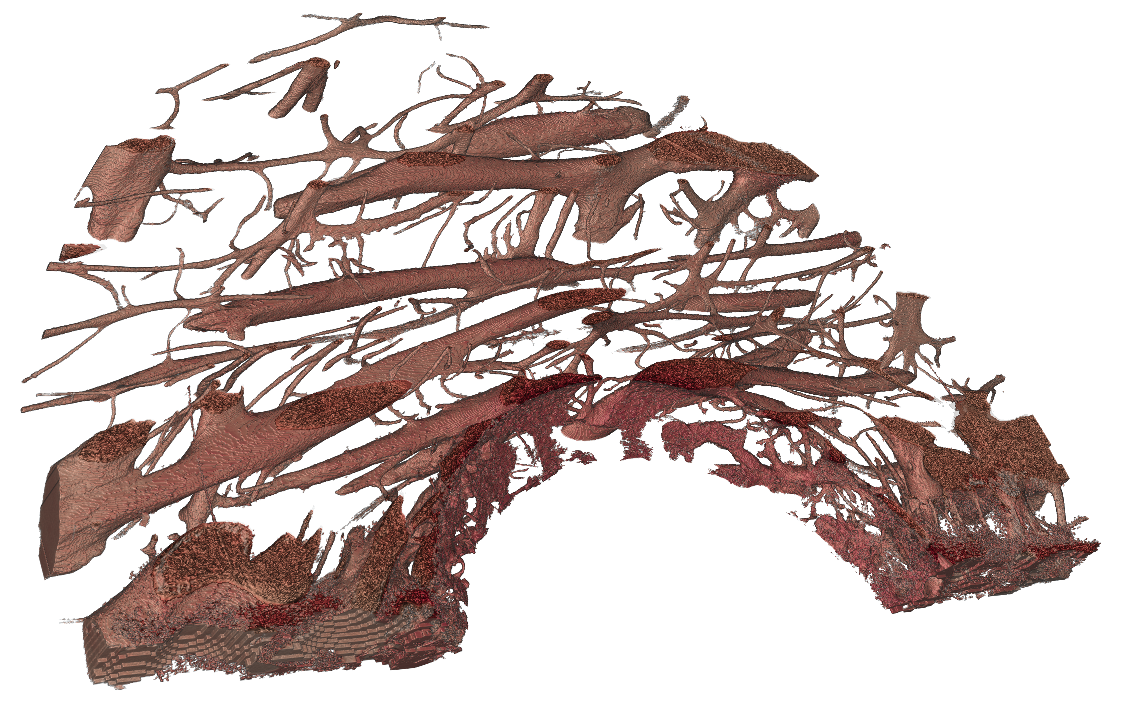
\includegraphics[width=.7\linewidth]{figures/blood_old_bone_100.png}
        % TODO opdater hvis en anden slice størrelse bliver brugt. voxel size = 3.75
        \caption{A $375\mu m \times 4230\mu m \times 6480\mu m$ slice of the blood network in the old bone region.}
        \label{fig:blood-old-slice}
    \end{subfigure}
    \begin{subfigure}[b]{\linewidth}
    \centering      
        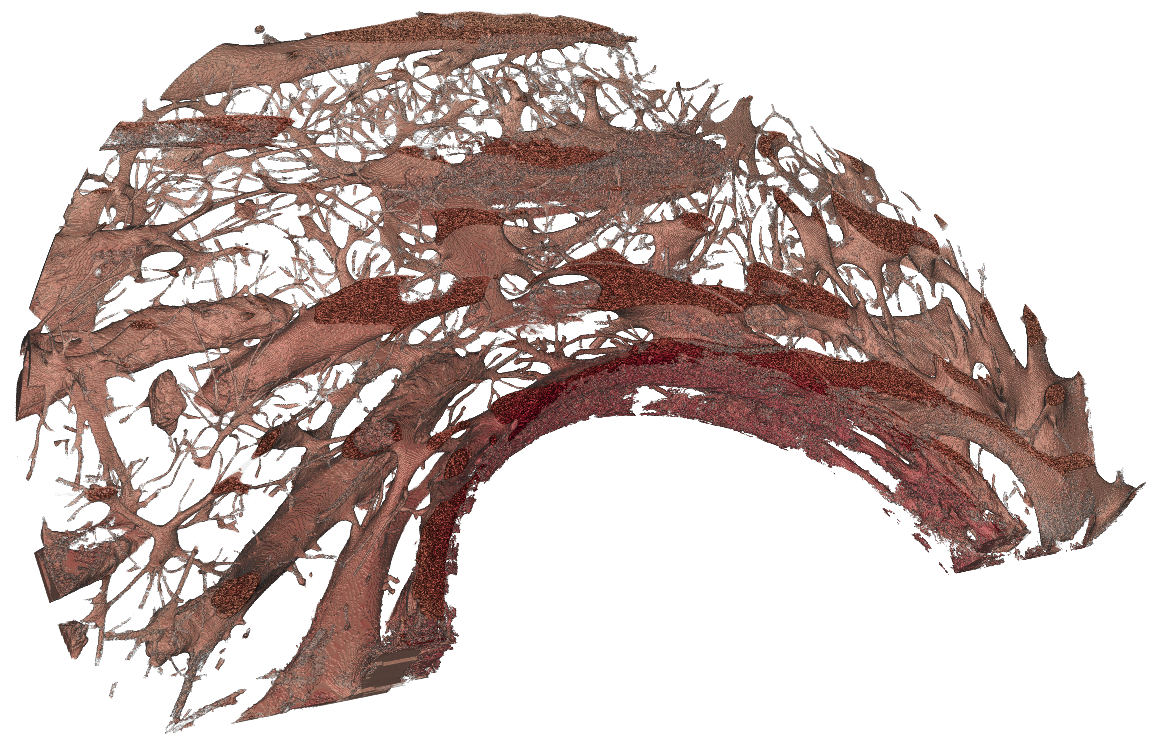
\includegraphics[width=.7\linewidth]{figures/blood_new_bone_100.png}
        \caption{A $375\mu m \times 4230\mu m \times 6480\mu m$ slice of the blood network in the new bone region.}
        \label{fig:blood-new-slice}
    \end{subfigure}
    \begin{subfigure}[b]{.48\linewidth}
    \centering      
        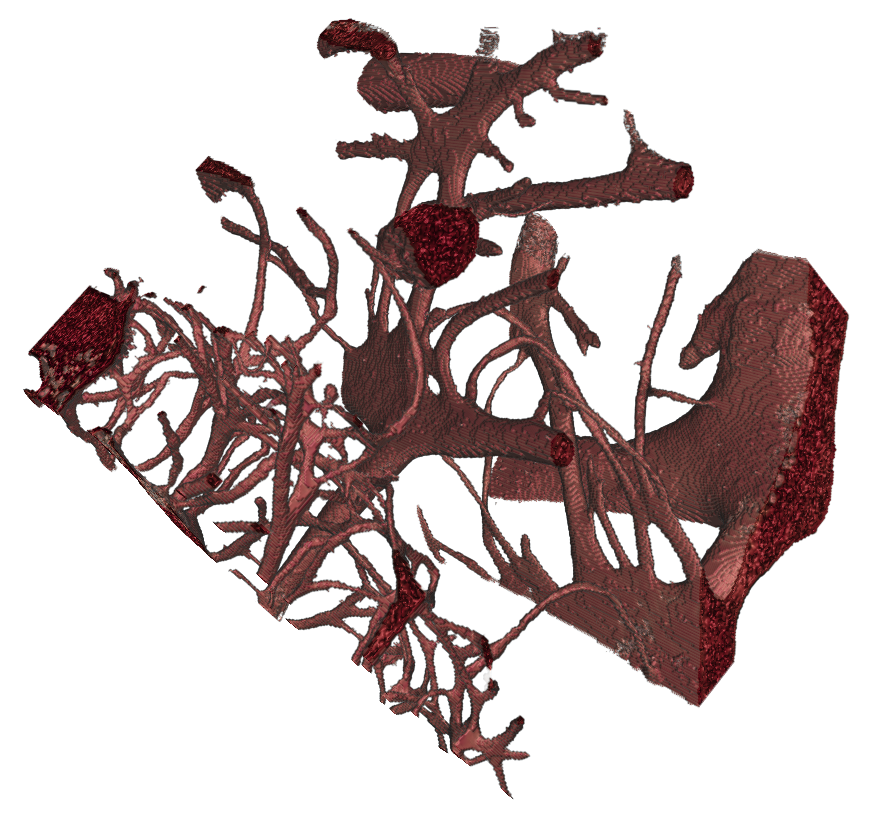
\includegraphics[width=.9\linewidth,height=\linewidth]{figures/blood_old_cube.png}
        \caption{A $1mm \times 1 mm \times 1 mm$ cube of the blood network in the old bone region.}
        \label{fig:blood-old-cube}
    \end{subfigure}
    \hfill
    \begin{subfigure}[b]{.48\linewidth}
    \centering      
        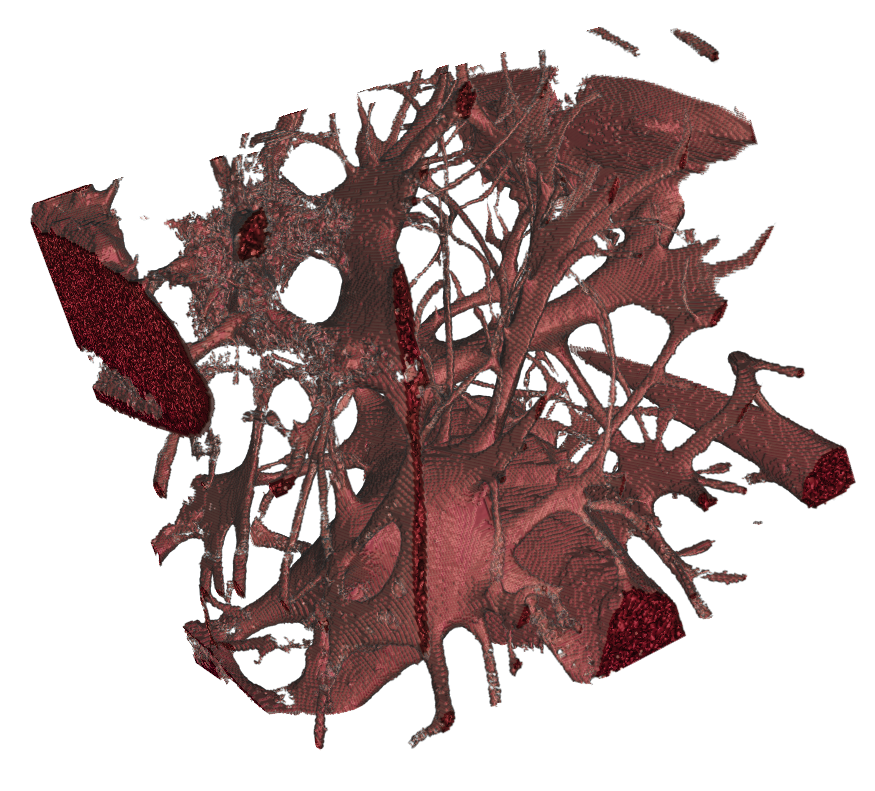
\includegraphics[width=.9\linewidth,height=\linewidth]{figures/blood_new_cube.png}
        \caption{A $1mm \times 1 mm \times 1 mm$ cube of the blood network in the new bone region.}
        \label{fig:blood-new-cube}
    \end{subfigure}
    \caption{3D renders of the blood network. Note the difference between the the capillary network in the old bone region (\ref{fig:blood-old-slice},\ref{fig:blood-old-cube}) compared to the newly grown bone region (\ref{fig:blood-new-slice},\ref{fig:blood-new-cube}).}
    \label{fig:blood-network}
\end{figure}

\subsubsection{Sub-classification of soft tissue}

With a good separation of soft tissue and bone, we map out the blood vessel network using connected
components analysis, which is visualized in the 3D renders in~\Cref{fig:blood-network}.
Here we see that we have successfully segmented the blood vessels out of the bone region.
It is especially prominent when looking at the capillary network, as we can see these in fine detail.
Noteworthy, the newly formed bone region (\Cref{fig:blood-new-slice}) contains a larger concentrations of these small blood vessels, compared to the old bone (\Cref{fig:blood-old-slice}).
If we zoom in to a small cube region (\Cref{fig:blood-old-cube} and \Cref{fig:blood-new-cube}), we see it even more defined, clearly seeing how the larger vessels connect through the smaller ones.

The osteocytes are selected by volume and shape: For every connected component
in the feasible volume range, its principal axis and best ellipsoid is computed and checked against
the potential osteocyte shape.

\subsection{Assessing bone-implant contact and blood-implant contact}

\begin{figure}
  \centering
  \begin{tabular}{c}
    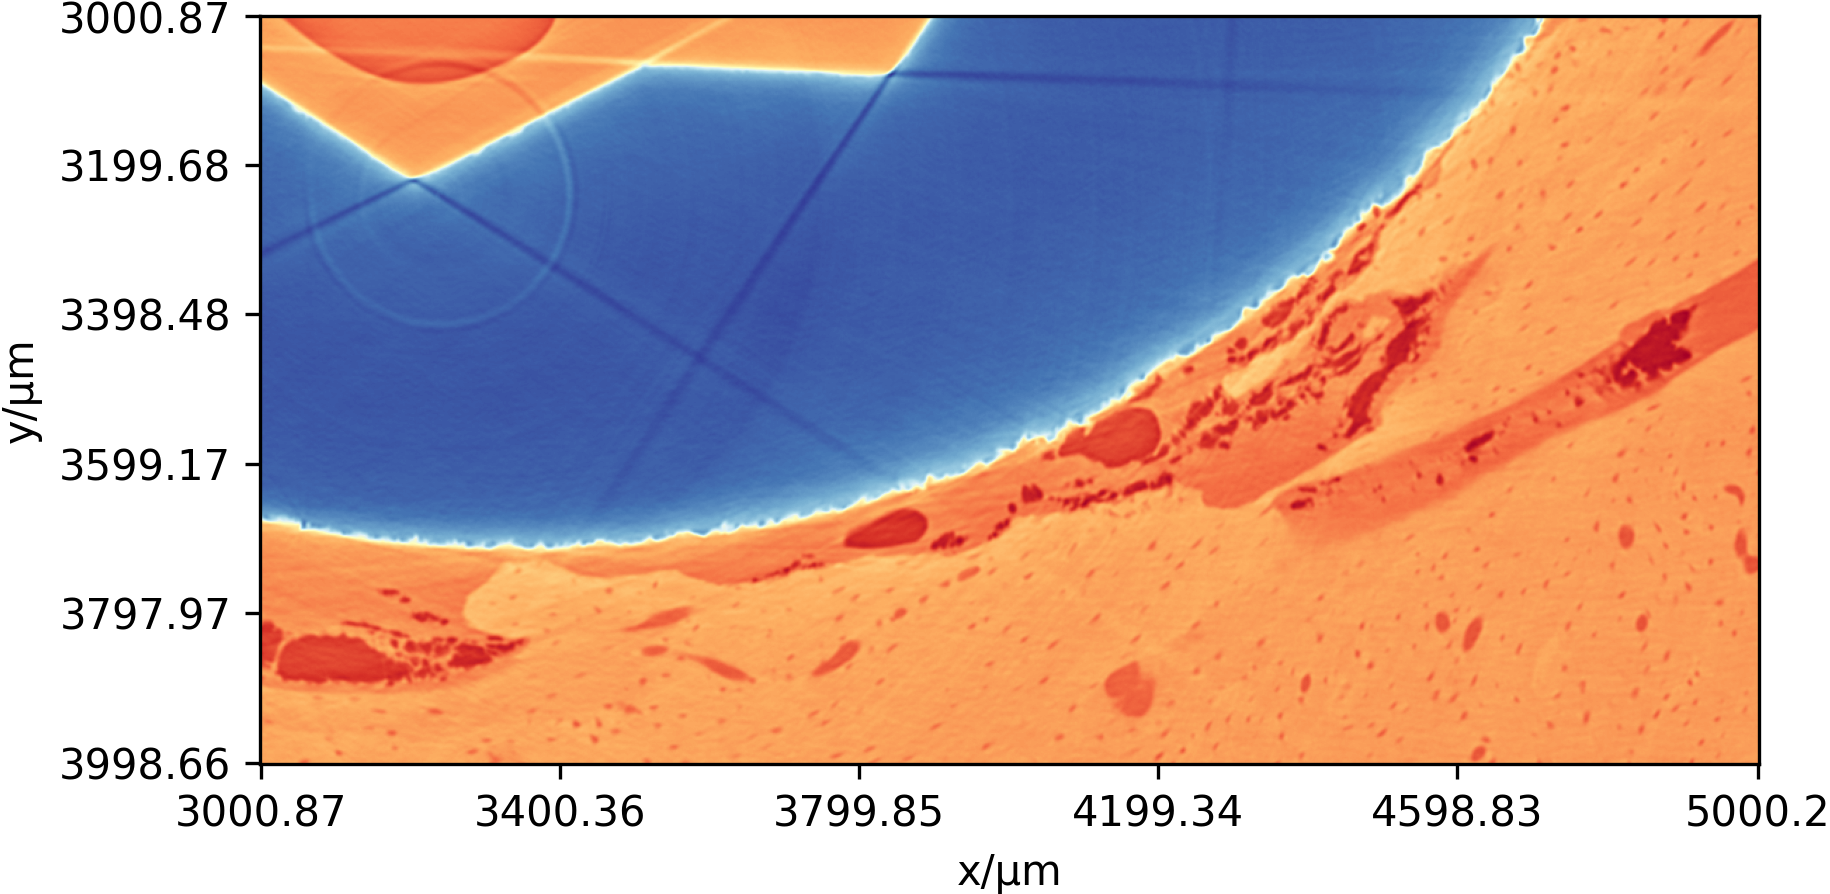
\includegraphics[width=\linewidth]{770c_pag-bic-xy-1x} \\
    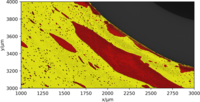
\includegraphics[width=\linewidth]{770c_pag-bic-P01-xy-1x}
  \end{tabular}
  \caption{XY slices of the original tomography (top), and the classified (bottom). The voxels are coloured according to the modeled probability functions $P(m\vert v,\fval)$ between 0 and 1: completely red voxels have $P(m=0\vert v,\fval) = 1$, completely yellow voxels have $P(m=1\vert v,\fval)\ = 1$, and uncertain voxels become progressively gray.
  }
  \label{fig:histology-comparison1}
\end{figure}

\begin{figure}
  \centering
  \begin{tabular}{c}
    \hspace{-0.5cm}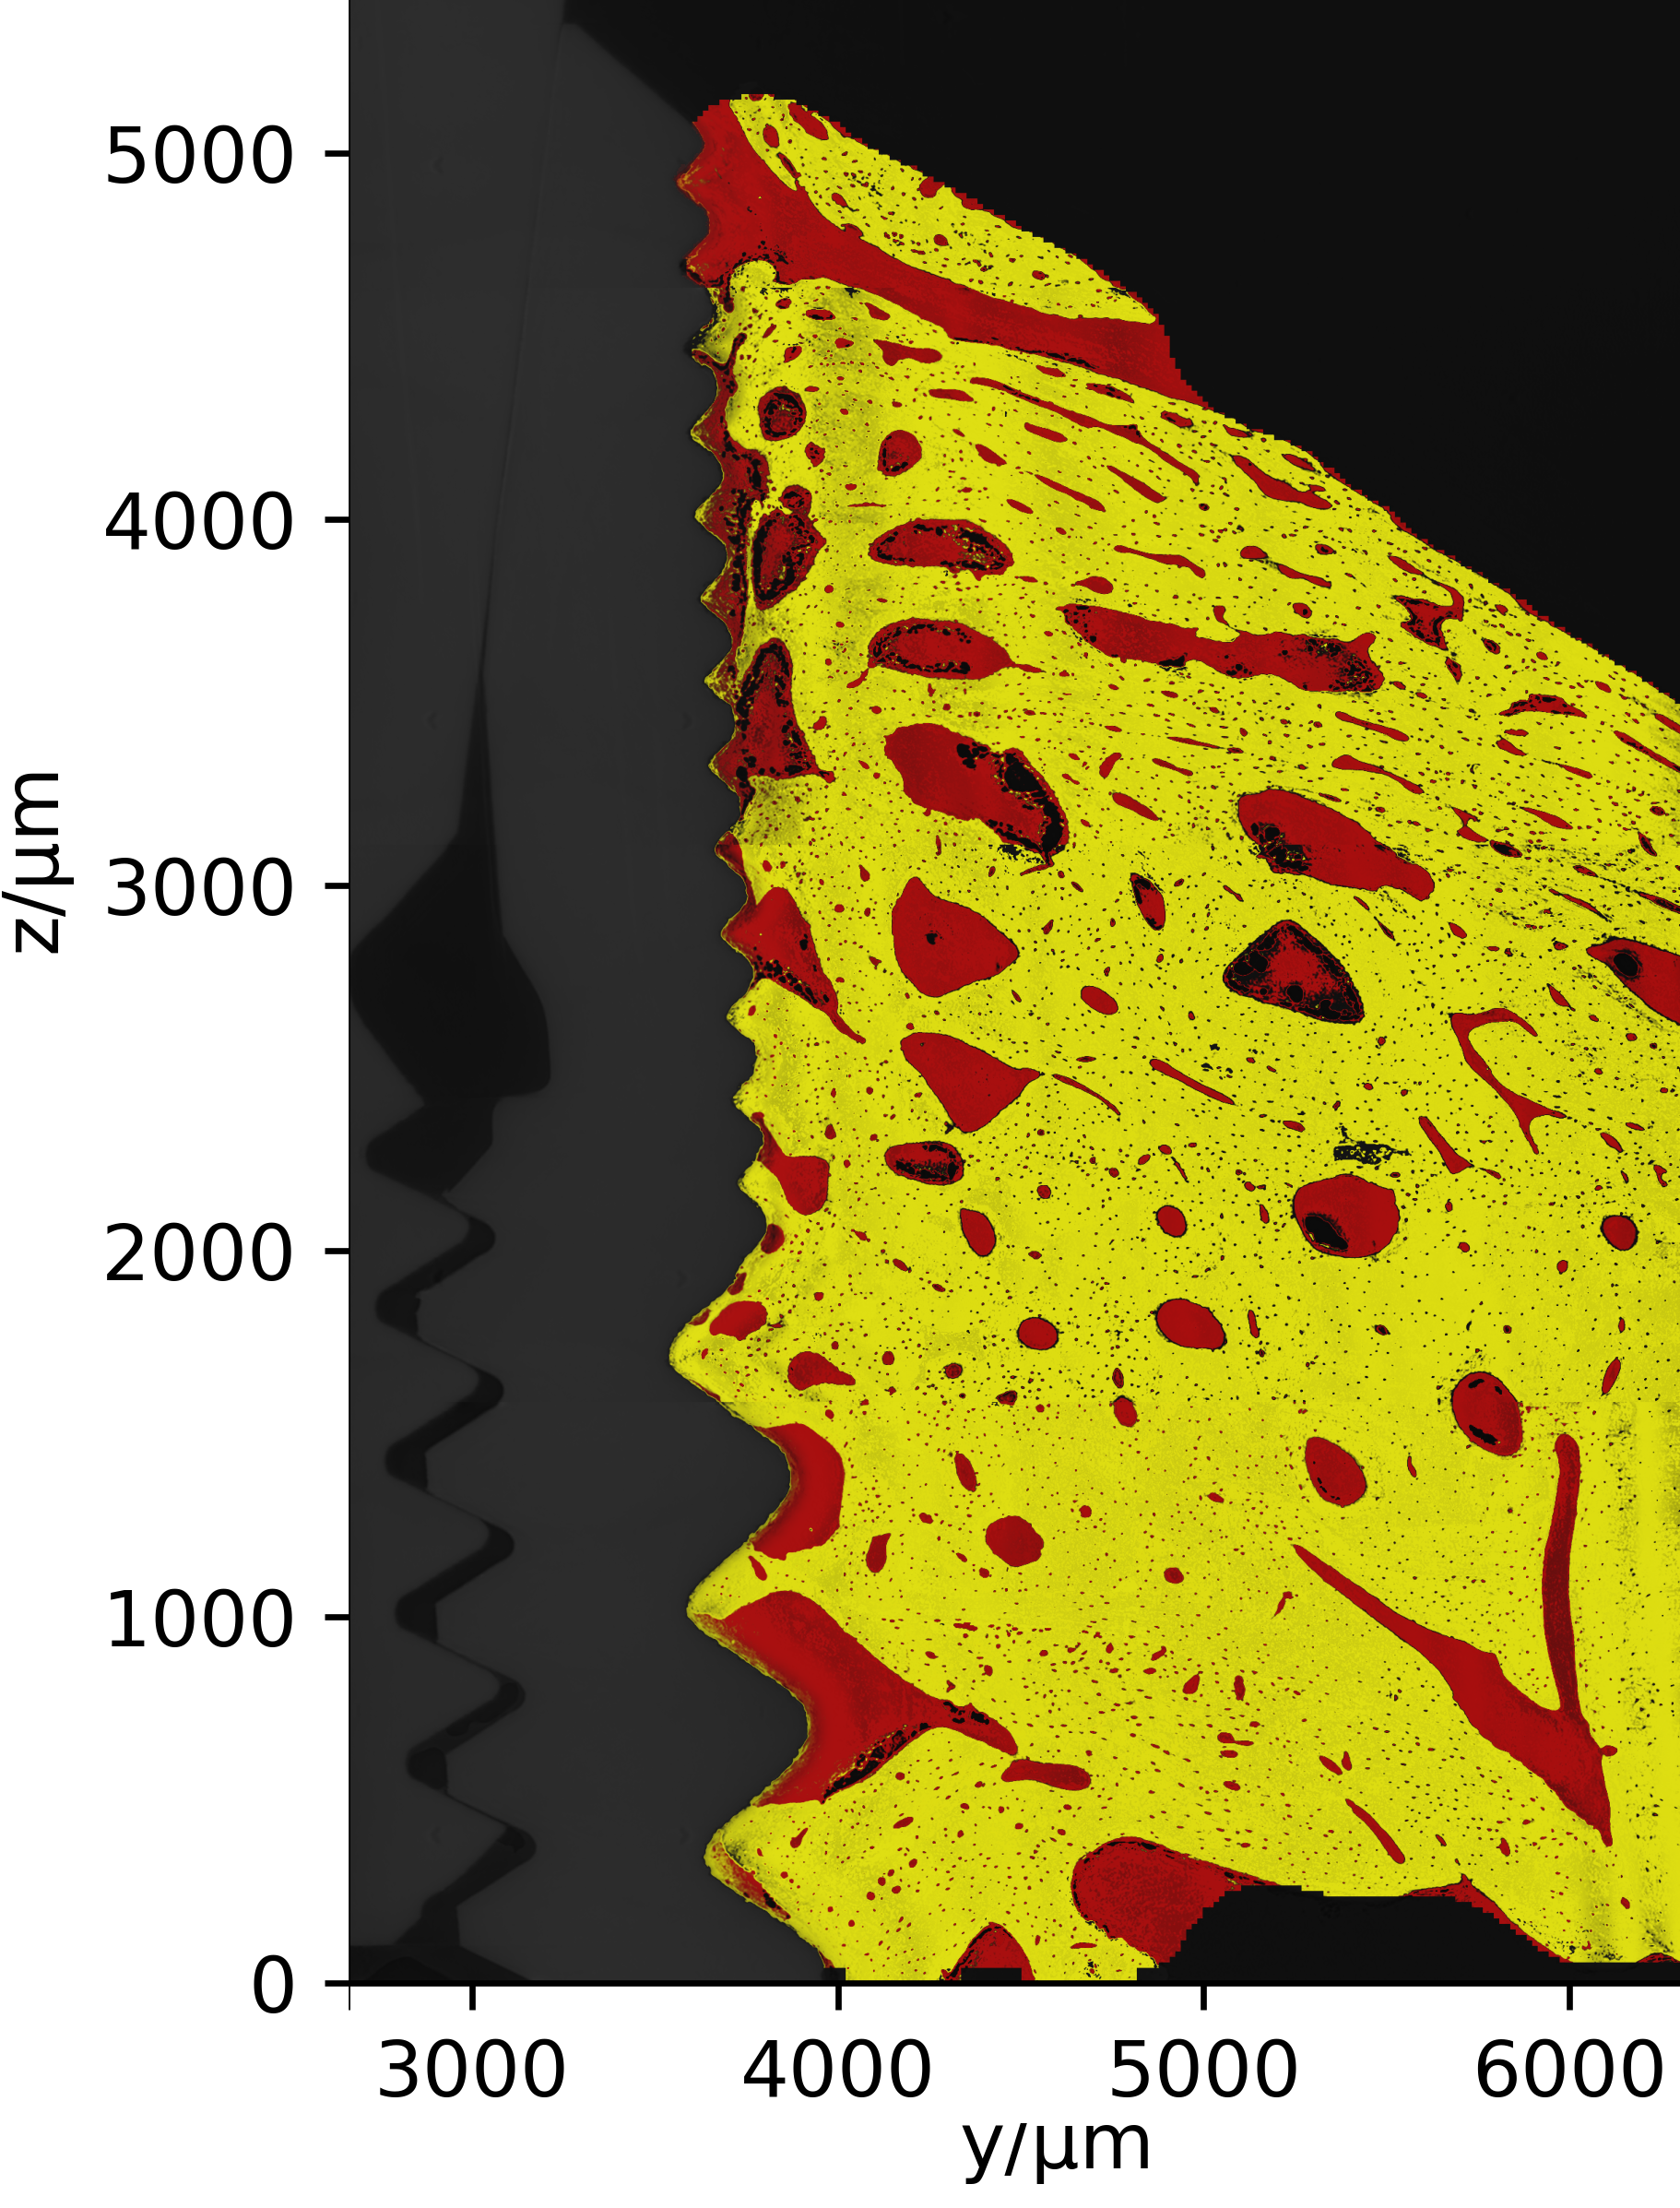
\includegraphics[width=.7\linewidth]{770c_pag-full-P01-yz-1x-gimp} \\
    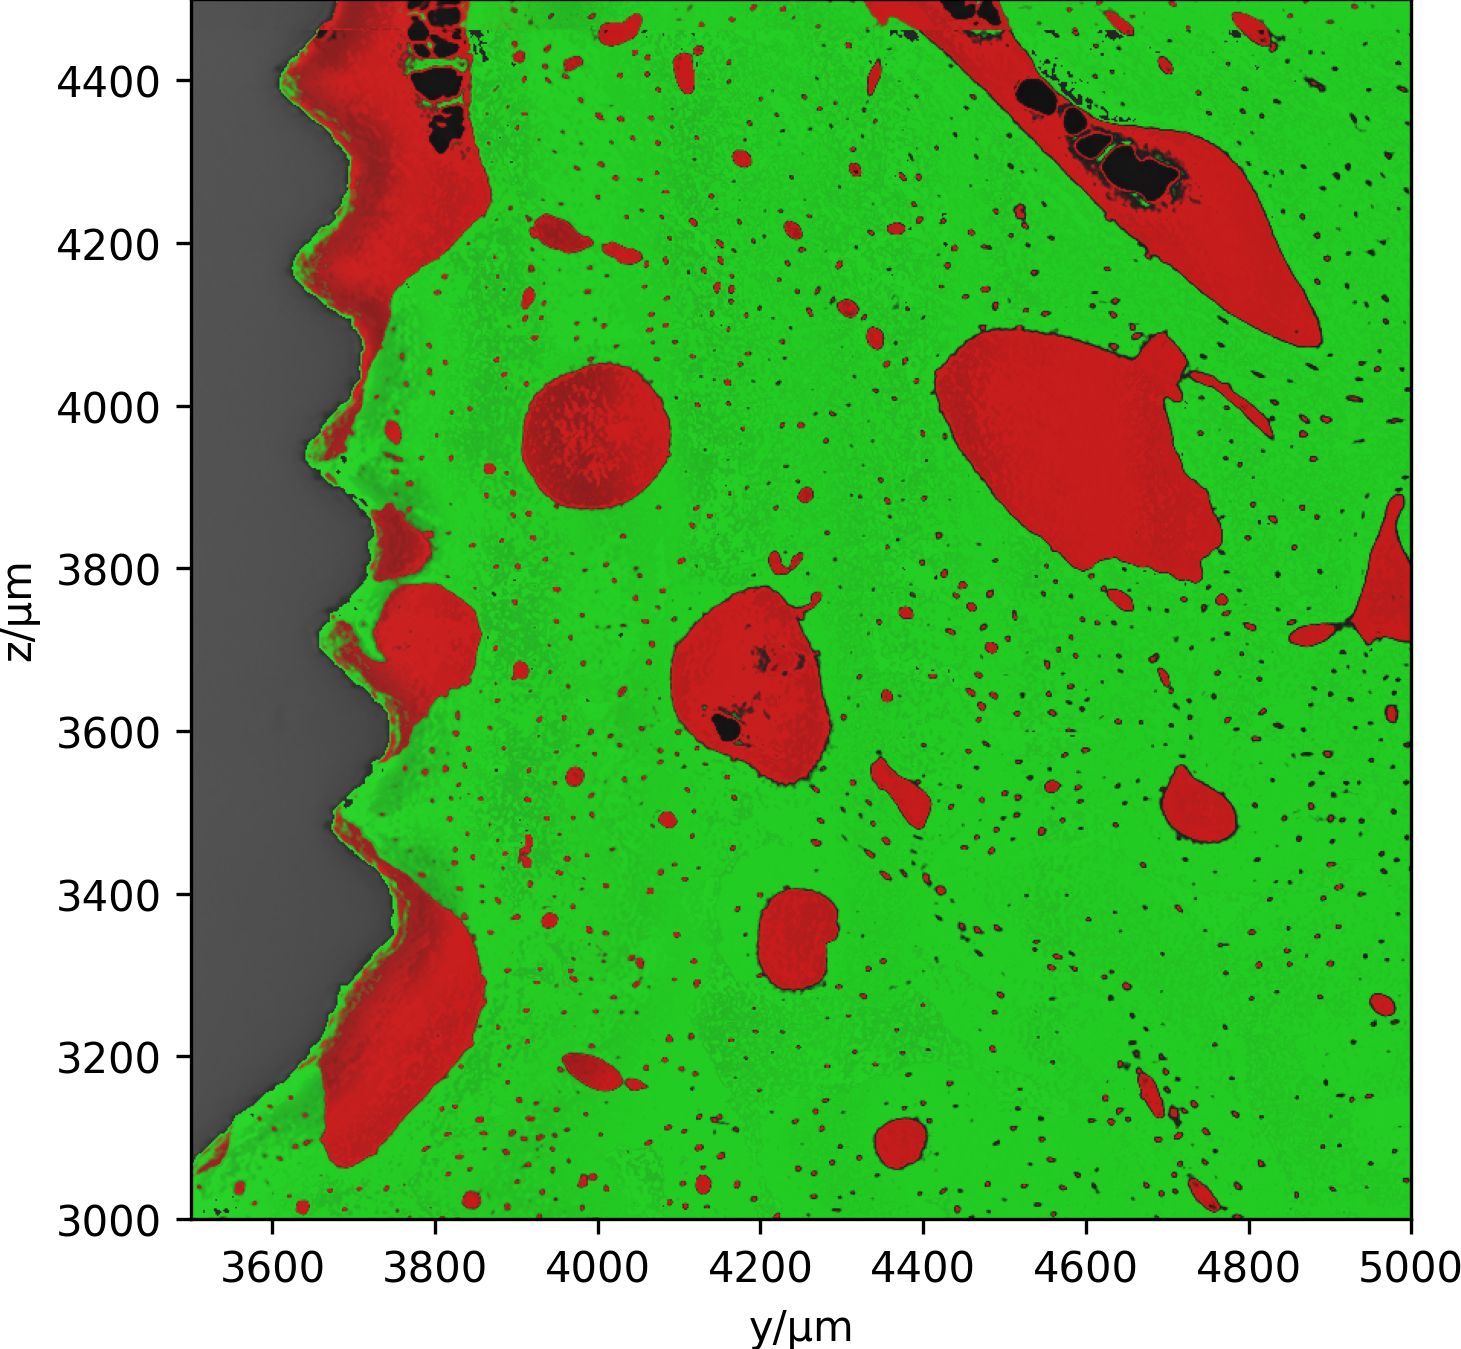
\includegraphics[width=.7\linewidth]{770c_pag-bic-P01-yz-1x}
  \end{tabular}
  \caption{ZY slices of the segmentation seen far away (top) and zoomed in (bottom). Yellow depicts bone and red depicts soft-tissue. Note that the segmentation correctly classifies the materials close to the implant, even in the grooves of the screw threads..}
  \label{fig:histology-comparison2}
\end{figure}


Once segmented, tissue in contact with the implant can be studied using the
Euclidean Distance Transform (EDT) from the implant, restricted to the bone region. We can
simply mask the voxels that are within a thin shell of distances, $d_{min} < d(x,y,z) \le d_{max}$,
for example $d_{min} = 1\mu m$ to $d_{max} = 5\mu m$. We then sum over the masked voxels of each
tissue type to obtain and divide by the total to obtain the tissue-to-implant contact per area,
or study the distribution across the surface area qualitatively. %TODO: Gør det!

A larger quantitative study is planned that analyses the full data set against recently conducted 
histological microscopy taken from the same biopsies. In the present work, we evaluate qualitatively:
Since the SR$\mu$CT tomograms are
clear enough that it is possible as humans to distinguish between blood vessels and bone,
as our mammalian visual cortex automatically corrects for the distortion effects, we can verify
the success of the automatic classification.

Figures \ref{fig:histology-comparison1} and \ref{fig:histology-comparison2} show the same 2D slices
as were shown in Figures \ref{fig:3viewsample} and \ref{fig:slices}, allowing us to visually inspect
them side by side. The voxels are coloured according to the segmentation confidence, with
degree of red proportional to the modeled probability $\Pof{0}{v,\fval}$ and degree of yellow proportional
to $\Pof{1}{v,\fval}$. Grey voxels indicate low model probabilities of both: either due to the voxel belonging
to another material, or simply low computed confidence of the model.
By comparing against Figures \ref{fig:histology-comparison1} and \ref{fig:histology-comparison2},
we see that the computed classification matches the human classification everywhere where it
is possible to visually distinguish the voxels. However, in a thin 1-voxel border
to the implant, we cannot verify the segmentation, as the voxel values are so blended together
with the implant voxel values that they become indistinguishable. A further strengthening of the analysis
is needed in order to reach this layer. It is possible that the information is irretrievably lost, or perhaps it
can be retrieved through a deconvolution - or simply a more precise version of the present analysis.


% \subsubsection{Cylindrical projection of implant contact-surface}

% In this subsection, we show how to map the tissue-to-implant contact surface for visual inspection.
% The challenge is that the equidistant region forms a curved surface that cannot simply be flattened.
% Instead, we project the voxels onto a cylinder, as shown in Figure \ref{fig:cylinder1}.

% \begin{figure}
%   \centering
%   \begin{tabular}{cc}
%     (a) & \begin{tabular}{c}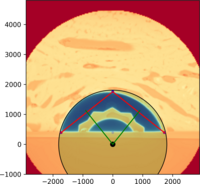
\includegraphics[width=.8\linewidth]{implant-FoR_prime-circle}\end{tabular} \\
%     (b) & \begin{tabular}{c}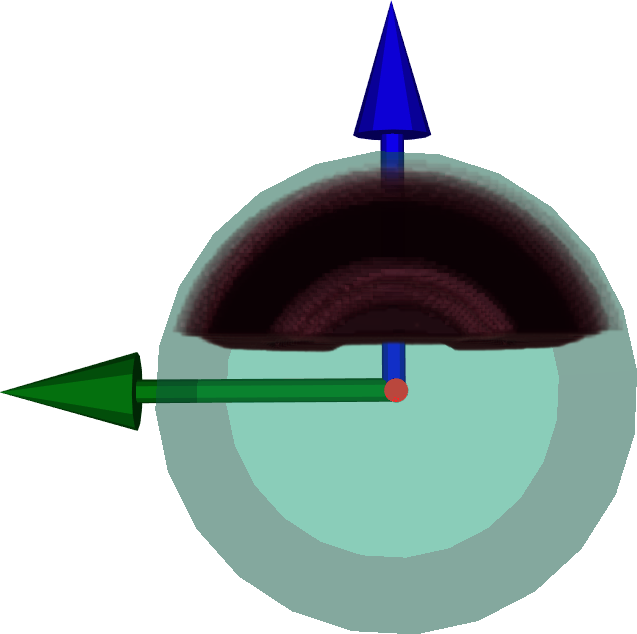
\includegraphics[width=0.4\linewidth]{implant-FoR_cylinder-y}%
%   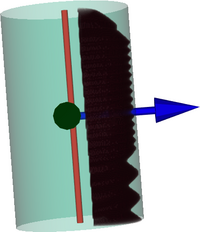
\includegraphics[width=0.5\linewidth]{implant-FoR_cylinder-z2}\end{tabular}
%   \end{tabular}
%   \caption{
%     (a) The implant is divided into 100 segments along its principal axis,
%     and for each segment, the circumscribed circle is computed.
%     (b) The best overall cylindrical fit for the implant is computed using
%     least squares. The implant contact is projected onto this cylinder,
%     and can now be shown in a flat plot.}
%   \label{fig:cylinder1}
% \end{figure}


\section{Conclusion and future work}
\label{sec:conclusion}

While SR$\mu$CT yields 3D reconstructions of extremely high fidelity compared to lab-grade X-ray setups,
several distortion effects remain that obstruct accurate tissue classification in important regions, in particular
near and at interfaces of high-contrast transitions such as where biological tissue meets metallic implants.
However, these effects are well behaved, in the sense that they vary smoothly over space, making it possible
to discover approximate mathematical models of the effects, and counter their resulting distortion.

We were able to build probabilistic models for the distortive effects
of soft tissue and bone voxel values as functions of distance to the
implant, and as functions of an approximate diffusion field. This made
it possible to see all the way up to the implant surface, and
automatically segment into tissue types throughout the sample and all
the way up to the implant surface, with high accuracy both at long and
short distances.

In this pilot work, we have only made a qualitative study. In upcoming
work, we plan a larger quantitative study that compares with histology
microscopy results, obtained from the same biopsies.  In addition, we
are extending the method with Bayesian combination of multiple
``angles'': different sources of distortion effects (e.g.~multiple
physical effects) can be better captured by different fields,
e.g.~beam hardening may be best captured by the distance transform to
the sample surface, while the diffusion field captures distortion near
metallic implants. Thus different fields separate tissue material
distributions in different regions, and in combination are expected to
yield a stronger analysis. It is hoped that this will make it possible
to separate multiple highly overlapping frequency distributions.


\section{Acknowledgements}

This project has received funding from the European Union’s Horizon 2020 research and innovation programme under grant agreement No. 779322 (``MAXIBONE'').
JA was partially supported by the VILLUM Foundation through VILLUM Experiment Project: 41017.
CJ was funded by the Innovation Fund Denmark (IFD) under File No. 8057-00012B, the IFD Grand Solutions project ``Adaptive X-ray InSpection''.

%\biboptions{authoryear}
\bibliography{refs}

\end{document}
